\documentclass[11pt, twoside]{report}
\usepackage[utf8]{inputenc}
\usepackage[margin=2.5cm]{geometry}
\usepackage{graphicx}  		% display images
\usepackage{rotating}
\usepackage{tikz} 
\usepackage[portuguese]{babel}
\usepackage{indentfirst}
\usepackage[colorlinks=true,linkcolor=black,urlcolor=black,bookmarksopen=true]{hyperref} % Make hyperlinks in index
\usepackage{bookmark} 		% Bookmarks for pdf file
\usepackage{float} 			% colocar as imegens e tabelas dentro do texto
\usepackage{fancyhdr}
\pagestyle{fancy}
\usepackage{tabularx} 		% x column in table can jump a line
\usepackage{setspace} 		% espçamento entre linhas
\usepackage{fancyhdr} 		% creates fancy footers and headers
\raggedbottom				% makes bottom of page more empy to make sure previous text doesnt have vertical gaps
\usepackage{ltablex}
\usepackage{pdflscape}
\usepackage{multirow}
\pagestyle{fancy}
\lfoot{{\footnotesize Tecnologias de Informação}}
\rfoot{{\footnotesize ESTGA}}
\rhead{PTDW}
\lfoot{Calendário de exames}


\renewcommand{\footrulewidth}{1pt}%criar uma linha no que separa o rodapé



\begin{document}
	
\onehalfspacing % espaçamento de 1,5 entre linhas

	
%	\lhead{Escola Superior de Tecnologia e Gestão de Águeda\\
%		Licenciatura em Tecnologias da Informação
%	}
	
	%\rhead{Capítulo \thechapter}
	\pagenumbering{roman}
	
	\begin{titlepage}
		\centering
		\scshape\Huge Calendário Exames\par
		\vspace{0.9cm}
		
		\scshape\large Projeto Temático em Desenvolvimento Web \\
		\vspace{0.3cm}
		\scshape\large 1º semestre de 2021/2022\par
		\vspace{0.4cm}
		\centering
		%\includegraphics[width=10cm]{}\par
		
		\vspace{1cm}
		
		\large
		Autores\\
		Gonçalo Tavares, Nº 92382  \\
		Bruno Lopes, Nº 86217 \\
		Leonardo Silva, Nº 95381 \\
		Ricardo Fernandes, Nº 49880 \\
		Sofia Rocha, Nº 99991 \\
		
		\vspace{1cm}
		
		\centering
		
\includegraphics[width=10cm]{image/AssB_vertical_cor.png}
		
		\newpage
		\thispagestyle{plain}%retira cabeçalho e rodape
		\thispagestyle{empty}%retira a numeração da pagina
		\centering
		\scshape\Huge Calendário Exames \par
		\vspace{1cm}
		
		\scshape\large Projeto Temático em Desenvolvimento Web\par
		\vspace{1cm}
		\scshape\large 1º semestre de 2021/2022\par
		\vspace{4cm}
		
		
		
		\large
		Autores\\
		Bruno Lopes, Nº 86217 \\
		Gonçalo Tavares, Nº 92382  \\
		Leonardo Silva, Nº 95381 \\
		Ricardo Fernandes, Nº 49880  \\
		Sofia Rocha, Nº 99991 \\
		
		\vspace{1cm}
		Orientadores\\
		Rita Santos \\
		Fábio Marques\\
		\vspace{4cm}
		
		\centering
		
\includegraphics[width=10cm]{image/AssB_vertical_cor}
		
	\end{titlepage}

	\newpage
	\setcounter{page}{1} % começa a contar a paginas no numero 1
	\tableofcontents % Índice de conteúdos
	\thispagestyle{plain} % retira cabeçalho e rodape
	\thispagestyle{empty} % retira a numeração da pagina
	\newpage
	\listoftables % Lista de tabelas
	\newpage
	\listoffigures % Lista de figuras
	
	\newpage
	\pagenumbering{arabic}
	
	\chapter{Introdução}
	
	No âmbito do Projeto Temático em Desenvolvimento Web associado às disciplinas Web Design e Desenvolvimento Web Multiplataforma foi proposto o desenvolvimento de uma aplicação web para solucionar a necessidade de um cliente. 
	O grupo constituinte deste projecto acordou abordar o tema de gestão de calendários de avaliações que consiste no desenvolvimento de uma aplicação web desenvolvida com as tecnologias web lecionadas no módulo temático que engloba este projecto.
	Este projecto servirá então como solução ao problema apresentado pelo cliente onde cada funcionalidade será feita mediante as necessidades apresentadas.
	
	Tipicamente quando se pensa num calendário imagina-se um sistema que organize o tempo na forma de anos, subdivididos em meses e por sua vez divididos em dias.
	Este sistema advém de costumes milenares praticados por várias religiões e civilizações antigas onde a forma mais básica de medir ciclos de tempo vem da observação da rotação do Sol por parte do observador que define um dia, as mudanças da fase da lua que traduz de uma forma bruta o passar de um mês e ainda a observação de estações do ano caracterizadas por eventos climáticos distintos que no seu conjunto formam um ano\cite{stray_mayan_2007}.
	
	Contudo a necessidade de organizar eventos numa escala mais curta de tempo conduz à reorganização de tempo de modo a catalogar acontecimentos associados a pequenos períodos de tempo. 
	A forma sócio-económica mais comum de organizar dias está no uso unitário de horas, ou períodos do dia caso seja essa a necessidade, e estes aparecem representados graficamente numa tabela\cite{10.1145/2702613.2732512} que divide o dia em blocos iguais por forma ao resultado da sua soma ser proporcional \cite{Russell1910-RUSPMV}. 
	Esta forma visual de divisão ajuda a que identificação da duração de um bloco seja facilmente interpretável quando vista de relance. 
	
	Com o avanço da tecnologia no século XX e a popularização do uso da Internet, os calendários tradicionais de papel foram gradualmente caindo em desuso dando lugar a calendário digitais que proporcionam numeras vantagens nomeadamente a portabilidade para todos os tipos de dispositivos modernos, maior complexidade de informação que é permitida armazenar nestes, possibilidade de partilhar calendários e agendas, etc.. 
	
	Hoje em dia o simples ato da criação de um calendário ou agenda digital tem em sî concentrado uma vasta panóplia de ferramentas para o fazer, quer seja no uso do calendário de um sistema operativo ou gestor de email que agenda tarefas e notifica antecipadamente, ou numa aplicação para telemóvel que junta a facilidade de uso de \textit{apps} com o design minimalista para a criação de uma agenda rápida ou ainda o uso de páginas \textit{web}, ou \textit{webapps} que pode ser acedido de qualquer dispositivo com capacidade para aceder à Internet. 
	
	De facto existem muitas formas de criar um calendário nos dias modernos, mas do ponto de vista de quem constrói a ferramenta em si, o princípio é o mesmo, o programador tem sempre de associar uma entidade representativa de um evento a uma hora/data de inicio sendo a duração desta decidida pelo utilizador final. 
	A forma final de apresentação dos resultados ficará no entanto à descrição do cliente/utilizador final que é para este que todo o desenvolvimento de apresentação e funcionalidades é desenvolvido por forma a satisfazer as necessidades.
	Mediante esta realidade a metodologia de trabalho foi baseada em reuniões pré preparadas com o cliente para perceber as necessidades deste, onde retiramos os objectivos principais e identificamos requisitos funcionais e não funcionais.
	São então desenvolvidas soluções baseadas na informação recolhida e posteriormente apresentadas ao cliente inicialmente na forma de protótipos de baixa fidelidade, \textit{wireframes}, e posteriormente versões funcionais de uma aplicação web com intuito de obtenção de \textit{feedback} durante o processo de desenvolvimento.
	
	Este relatório está dividido em vários capítulos começando pela introdução que contém uma apresentação breve do evoluir histórico do uso desta ferramenta até às aplicações mais modernas, onde se enquadra a solução que será apresentada ao cliente.
	O conjunto dos capítulos seguintes serão dedicados ao planeamento do projeto, englobando planeamento ds várias fases do projeto, casos de uso discutidos com o cliente, requisitos funcionais e não funcionais e casos de utilização.
	A pré implementação está num capítulo dedicado à prototipagem e na implementação é abordado o modelo de dados persistentes, a implementação do protótipo de alta fidelidade funcional e as funcionalidades da aplicação, seguido dos testes de funcionamento das mesmas e pro fim a análise dos resultados e conclusão .
	
	\section{Objetivos da aplicação}
	
	Este projeto tem como principal objetivo a criação de uma aplicação web para solucionar a necessidade de um cliente que pretende um sistema de criação de calendários digitais para agendamento de um período de avaliações académicas num estabelecimento de ensino superior. 
	
	Sendo assim a aplicação tem de satisfazer os seguintes objetivos para a \textit{webapp}: 
	\begin{itemize} 
		\item \textit{Webapp} de fácil navegação e intuitiva para a criação de um calendário. 
		\item Possibilidade de agendamento de exames a unidades curriculares separados por curso, ano letivo e semestre.   
		\item Possibilidade de edição de curso, do docente, unidades curriculares, salas e o seu tipo. 
		\item Exportação de calendários para formato pdf e csv. 
	\end{itemize} 
	\section{Estado de arte}
	\label{estadodearte}
	
	A partir de uma pequena introdução do tema foi feita uma pesquisa sobre aplicações semelhantes para discutir com o cliente sobre a aplicação a ser criada. A pesquisa resultou em quatro aplicações: uma em versão mobile, uma em versão web e duas que dispõem de ambas as versões.
	
	A primeira aplicação, que se chama ``Timetable'' que tem como objetivo organizar todas as aulas, exames e tarefas escolares de um aluno. O utilizador pode adicionar aulas e exames (ver figura \ref{inserirvizualizaraula}), indicando a sala, o nome da disciplina, a data de início e fim, o nome do docente, o tipo e o dia da semana em que se realiza, sendo diferenciados pela frequência - as aulas são repetidas a cada semana e o exame só se realiza uma vez. Para além disso o aluno pode associar tarefas tanto a aulas como a exames podendo vizualizar estas informações em forma de lista ou em forma de calendário, como está apresentado na figura \ref{dayweekview}.
		\begin{figure}[H] 
		\centering 
		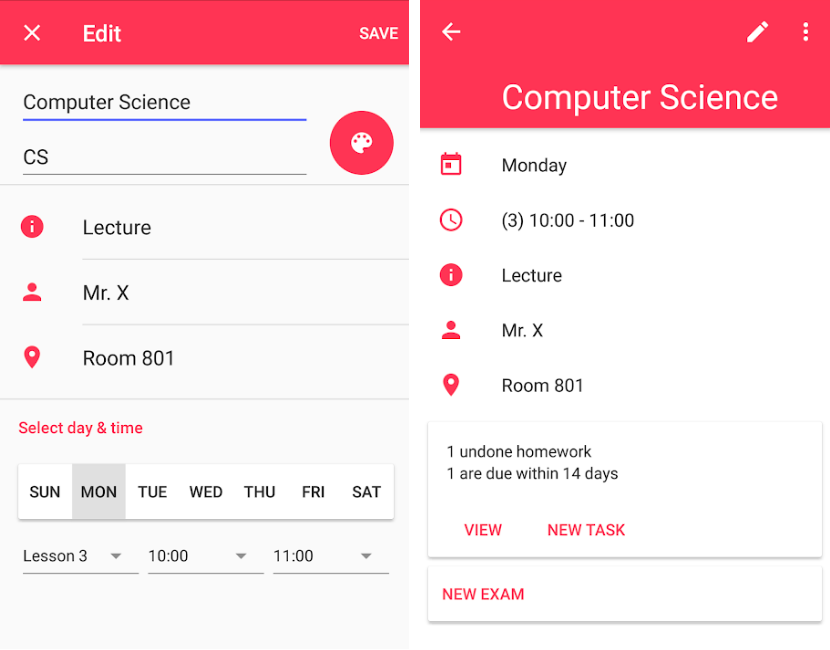
\includegraphics[width=0.7\textwidth,height=0.7\textheight,keepaspectratio]{image/estadodearte/inserirevizualizar}
		\caption{Inserir e vizualizar a aula adicionada}
		\label{inserirvizualizaraula}
	\end{figure}

	\begin{figure}[H] 
		\centering 
		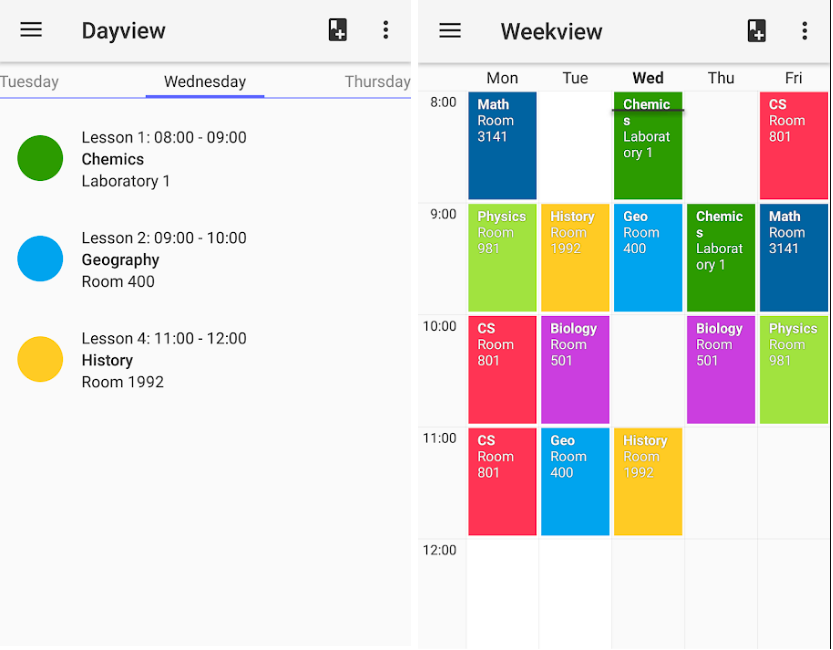
\includegraphics[width=0.7\textwidth,height=0.7\textheight,keepaspectratio]{image/estadodearte/dayweekview}
		\caption{Lista de aulas e o calendário escolar semanal}
		\label{dayweekview}
	\end{figure}

	A segunda aplicação ``StudyLife'' tem o mesmo objetivo que a aplicação anterior no entanto a sua apresentação gráfica é diferente, como se pode ver na figura \ref{listastudylife}. Poderá criar tarefas e exames associados a disciplinas, previamente criadas. Para cada tarefa pode indicar qual é a sua percentagem de realização e nos exames pode-se visualizar o dia e a hora do mesmo, a sala onde se realizará o exame, se existe conflitos com aulas e quanto tempo o aluno tem para o realizar (ver figura \ref{examematematica}). Estas informações podem ser vistas em forma de lista, apresentada na figura \ref{listastudylife} ou em forma de calendário semanal como se pode ver na figura \ref{calendariostudylife}.	
	
\begin{figure}[H] 
	\centering 
	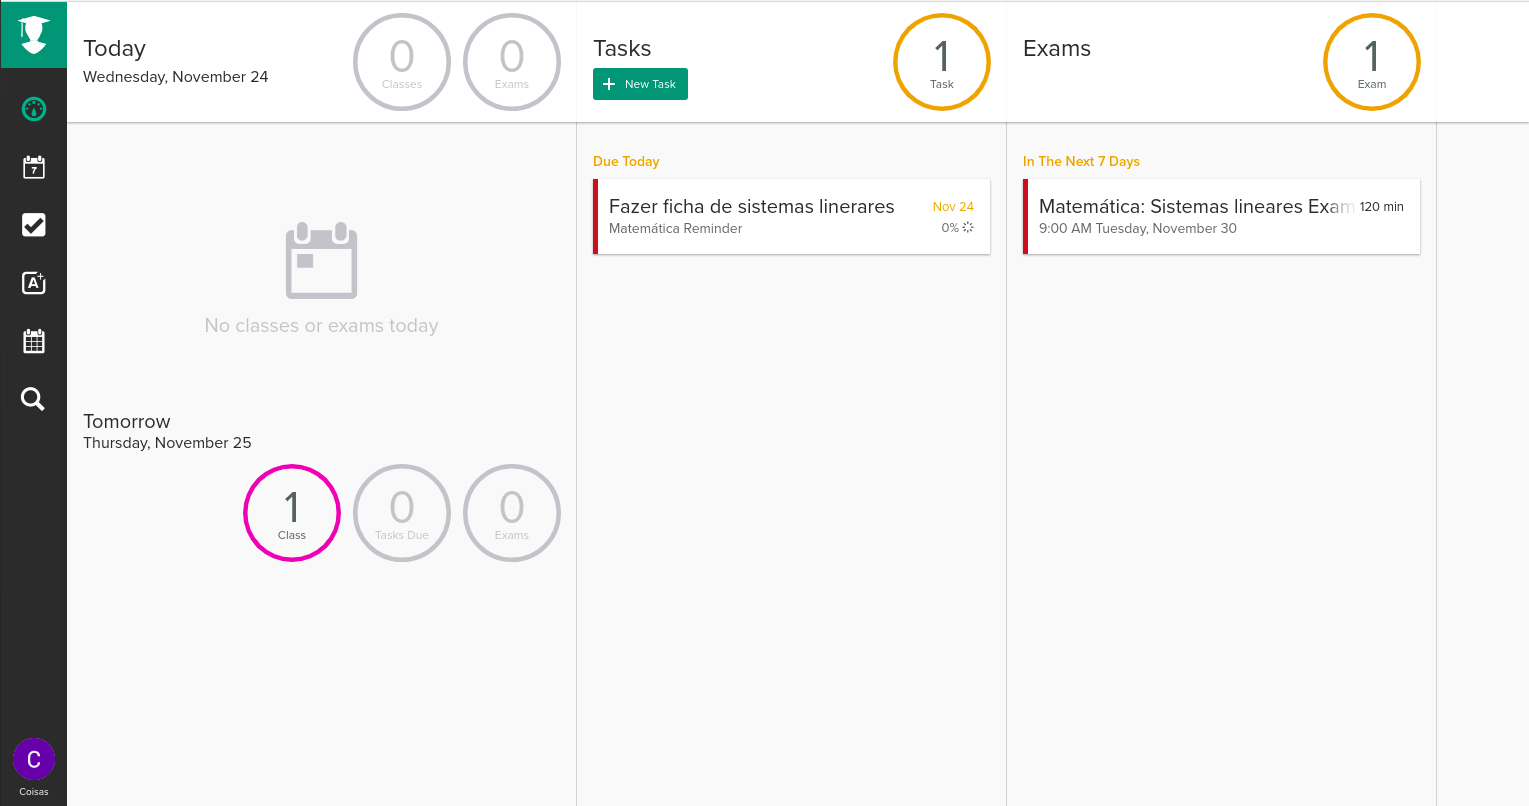
\includegraphics[width=0.8\textwidth,height=0.8\textheight,keepaspectratio]{image/estadodearte/calendario}
	\caption{Lista de tarefas e exames}
	\label{listastudylife}
\end{figure}

\begin{figure}[H] 
	\centering 
	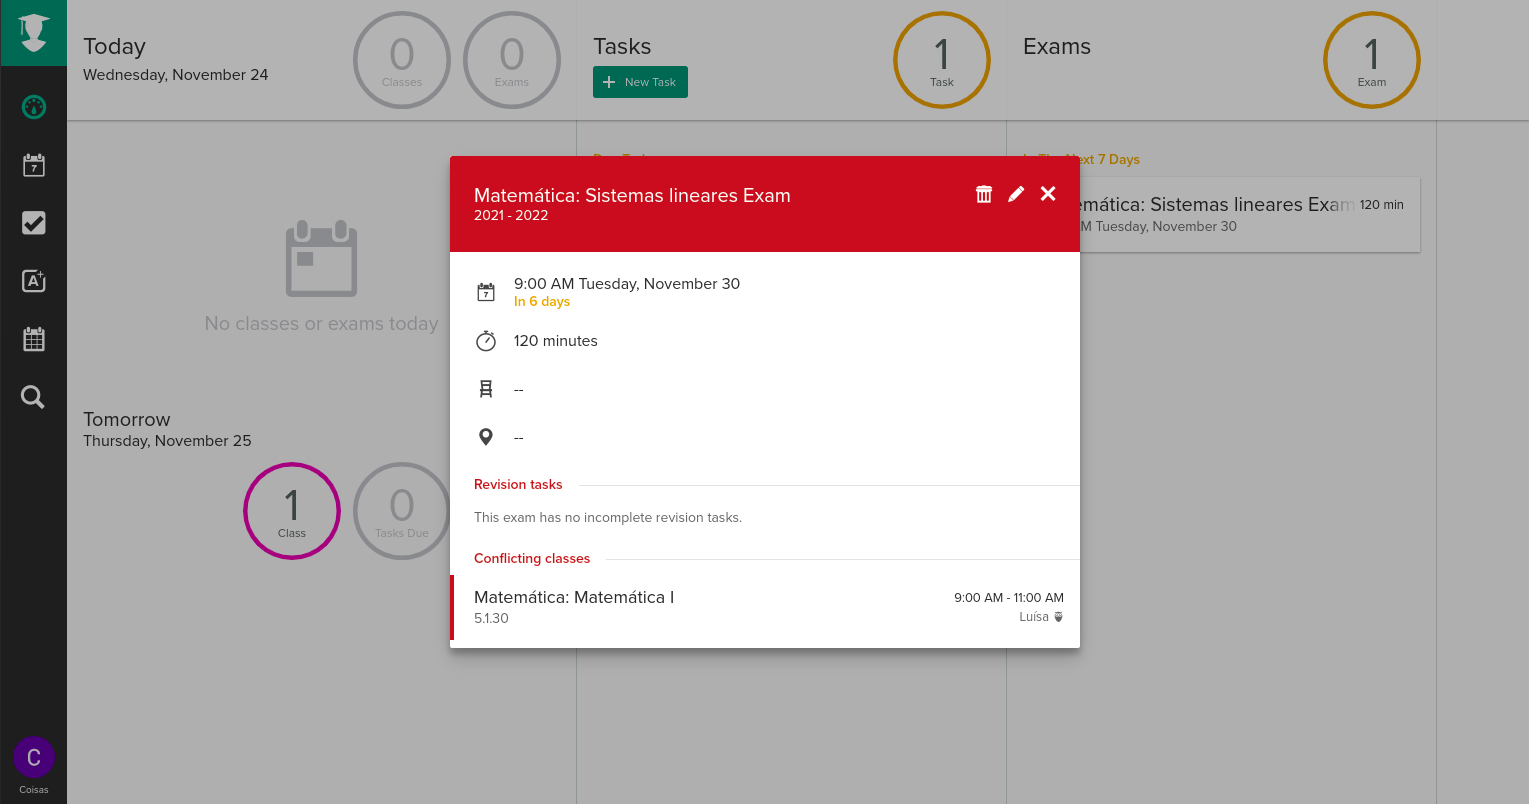
\includegraphics[width=0.8\textwidth,height=0.8\textheight,keepaspectratio]{image/estadodearte/informacoesexame}
	\caption{Visualização de informações sobre o exame de Matemática}
	\label{examematematica}
\end{figure}

\begin{figure}[H] 
	\centering 
	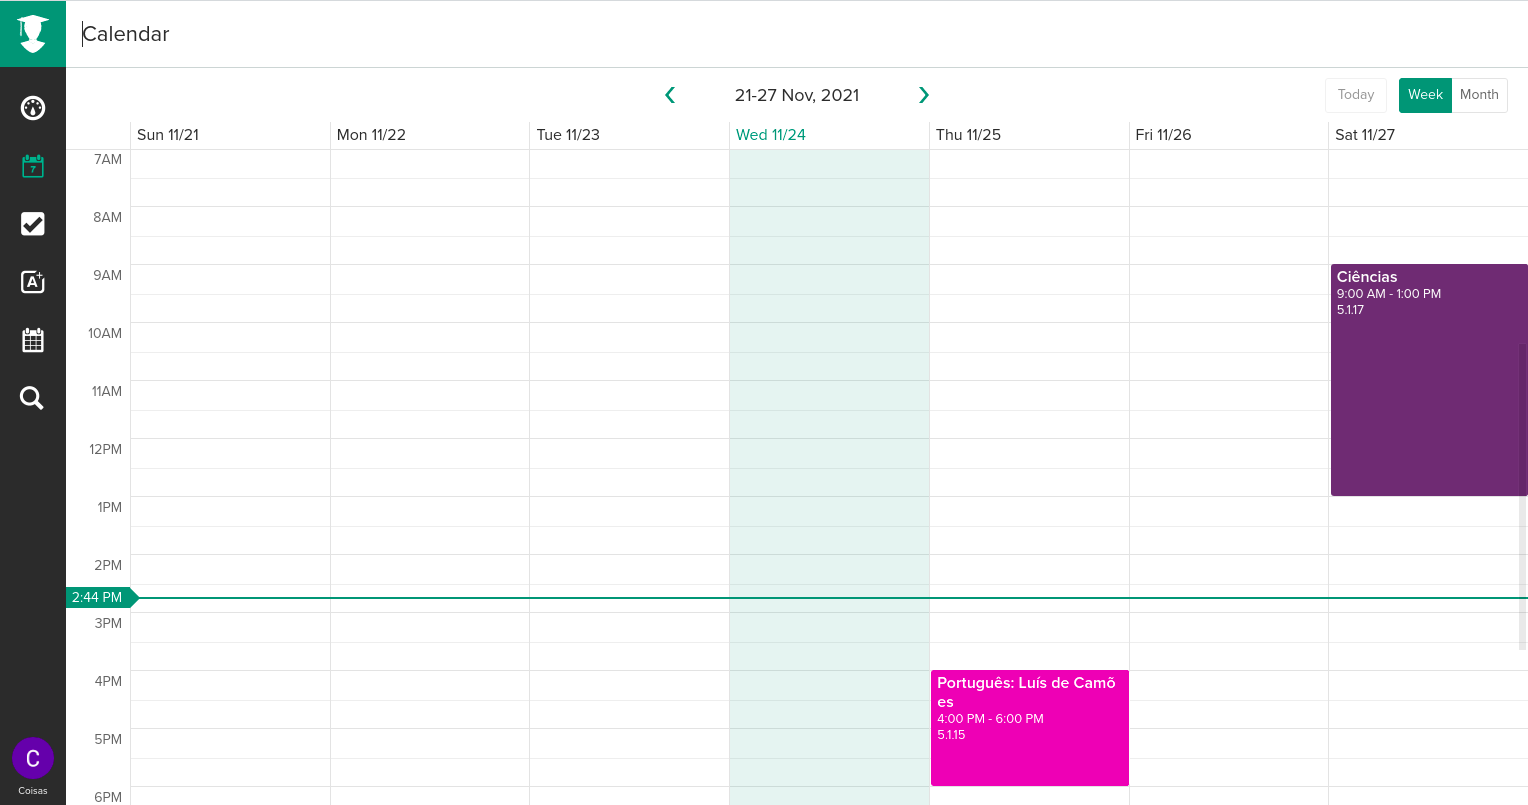
\includegraphics[width=0.8\textwidth,height=0.8\textheight,keepaspectratio]{image/estadodearte/calendariostudy}
	\caption{Visualização de informações em forma de calendário semanal}
	\label{calendariostudylife}
\end{figure}

	A terceira e a quarta aplicação foram selecionadas pela semelhança no conceito das mesmas face ao nosso projeto, sendo estas o ``Google Calendar'' e o ``Outlook Calendar", ambas têm um funcionamento semelhante, sendo concorrentes diretas uma da outra. Dispõem tanto de uma versão web como de uma versão mobile, no entanto iremos apenas abordar a versão web.

	Em ambas as aplicações é possível visualizar os conteúdos por dia, semana, mês ou ano e existe uma funcionalidade que nos permite criar diferentes calendários, sendo possível posteriormente adicionar eventos aos mesmos e alterar a visualização entre eles. Na figura \ref{googlecalendar}, referente à criação do calendário na aplicação da Google, podemos observar que esta permite a associação de um nome, descrição e fuso horário. No caso do Outlook, presente na figura \ref{calendariooutlook}, tem também a possibilidade de escolher a cor e um ícone, porém não existe um campo para associar uma descrição.

	\begin{figure}[H] 
		\centering
		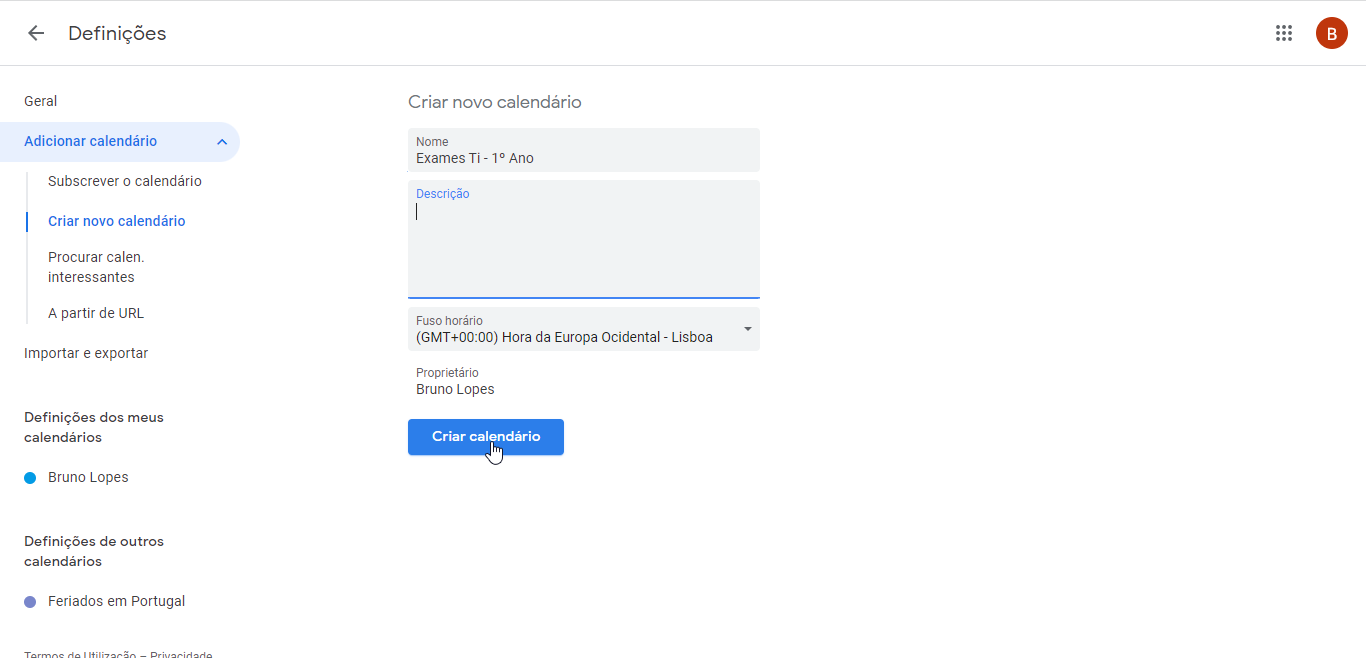
\includegraphics[width=0.8\textwidth,height=0.8\textheight,keepaspectratio]{image/estadodearte/criacao_calendario_google}
		\caption{Criação de um novo calendário no Google Calendar}
		\label{googlecalendar}
	\end{figure}

	\begin{figure}[H] 
		\centering
		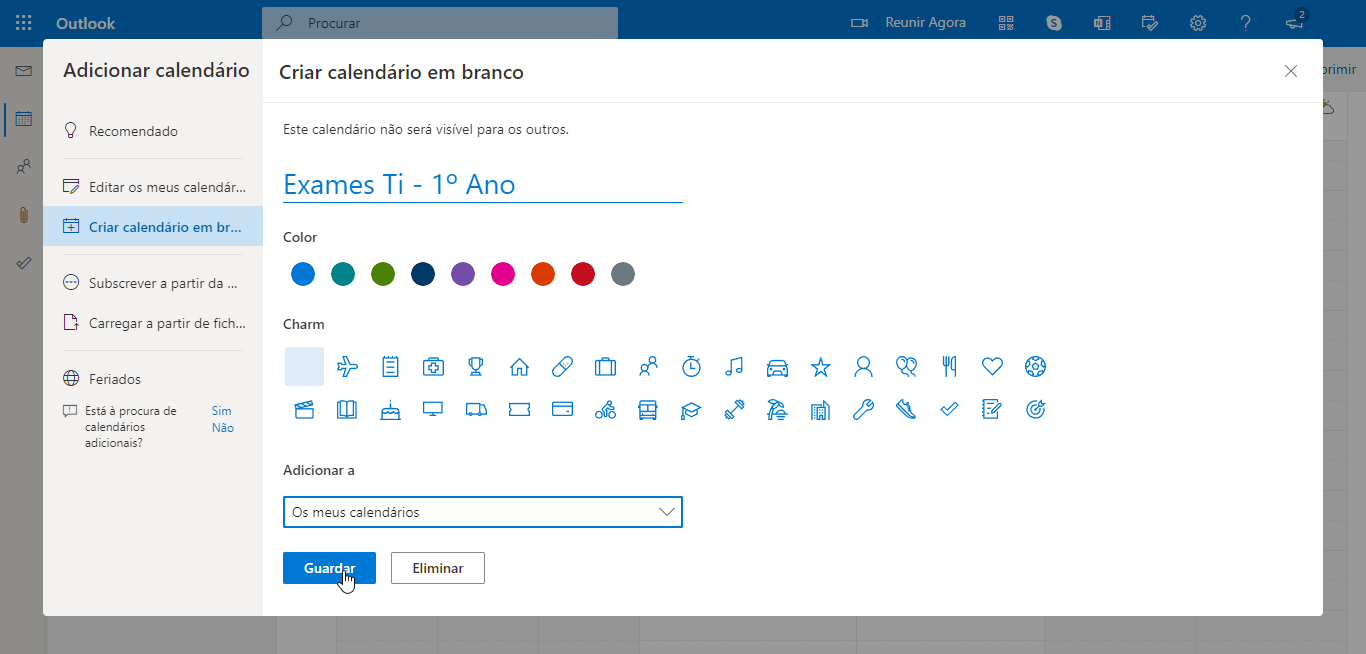
\includegraphics[width=0.8\textwidth,height=0.8\textheight,keepaspectratio]{image/estadodearte/criacao_calendario_outlook}
		\caption{Criação de um novo calendário no Outlook Calendar}
		\label{calendariooutlook}
	\end{figure}

	No caso do ``Google Calendar'', o utilizador pode adicionar eventos, tarefas e lembretes ao calendário através do botão criar ou ao selecionar/arrastar uma área diretamente no calendário. Porém o funcionamento das tarefas é semelhante a dos lembretes sendo que estes apenas permitem selecionar uma hora específica ou o dia inteiro. No entanto, conforme se pode observar na figura \ref{googlenovoevento}, aquando a criação de um novo evento é permitido ao utilizador selecionar um período de horas, onde temos diversos campos para preenchimento, entre os quais um título, datas/horas, convidados, local, descrição, repetição do evento, etc..

	\begin{figure}[H] 
		\centering
		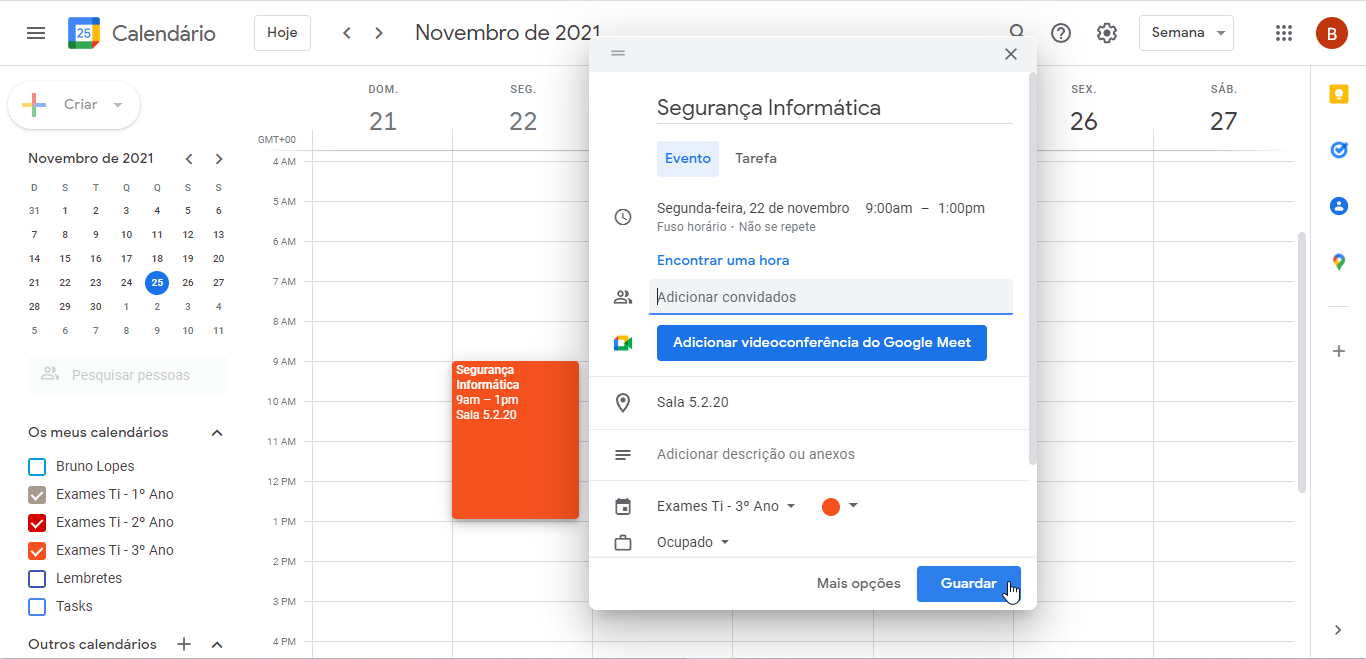
\includegraphics[width=0.8\textwidth,height=0.8\textheight,keepaspectratio]{image/estadodearte/criacao_evento_google}
		\caption{Criação de um novo evento no Google Calendar}
		\label{googlenovoevento}
	\end{figure}

	No caso do ``Outlook Calendar'', tal como a figura \ref{outlookevento} mostra, apenas é possível criar novos eventos, porém à semelhança do ``Google Calendar'' o utilizador pode proceder à criação dos mesmos recorrendo a um botão existente para o efeito ou ao selecionar/arrastar uma área no calendário, tendo também diversos campos para preenchimento entre os quais o título, participantes, datas/horas, repetição do evento, etc..

	\begin{figure}[H] 
		\centering
		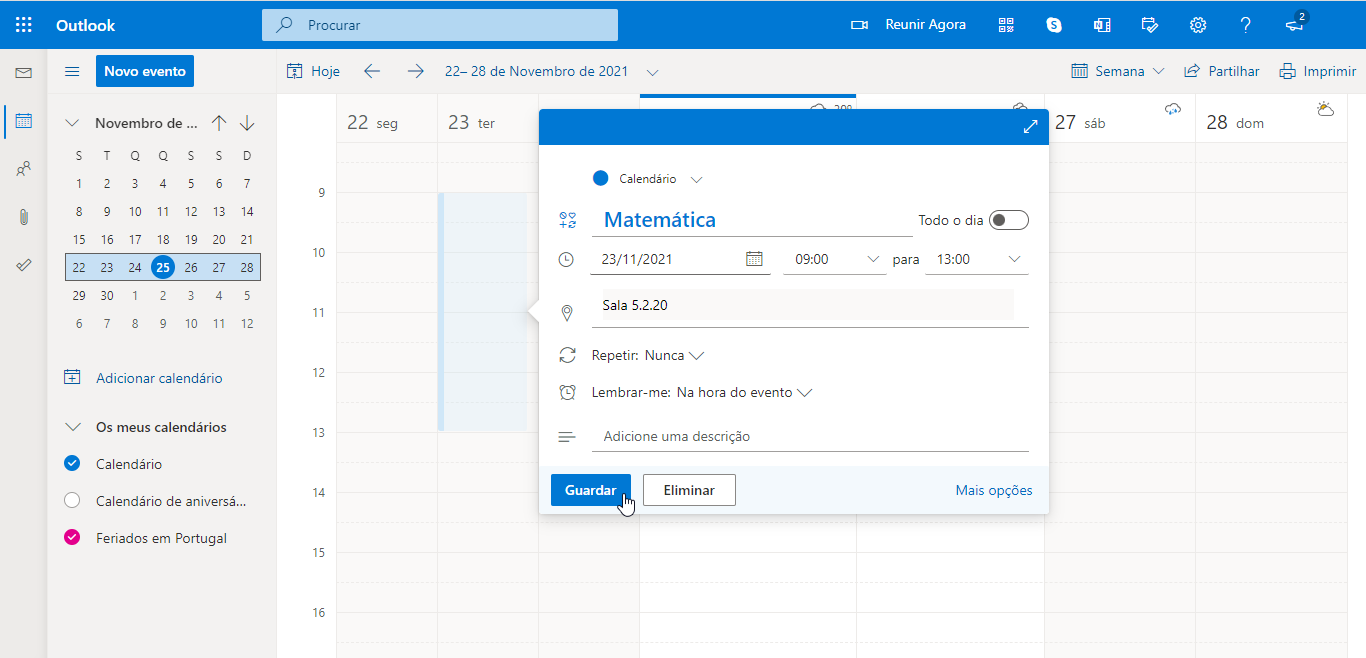
\includegraphics[width=0.8\textwidth,height=0.8\textheight,keepaspectratio]{image/estadodearte/criacao_evento_outlook}
		\caption{Criação de um novo evento no Outlook Calendar}
		\label{outlookevento}
	\end{figure}

Em ambas as aplicações após um evento ter sido criado no calendário é possível arrastar o mesmo para outro horário recorrendo à funcionalidade de ``Drag and Drop'' que ambos incorporam (ver figura \ref{googledragdrop} e \ref{outlookdragdrop}).\\

	\begin{figure}[H] 
		\centering
		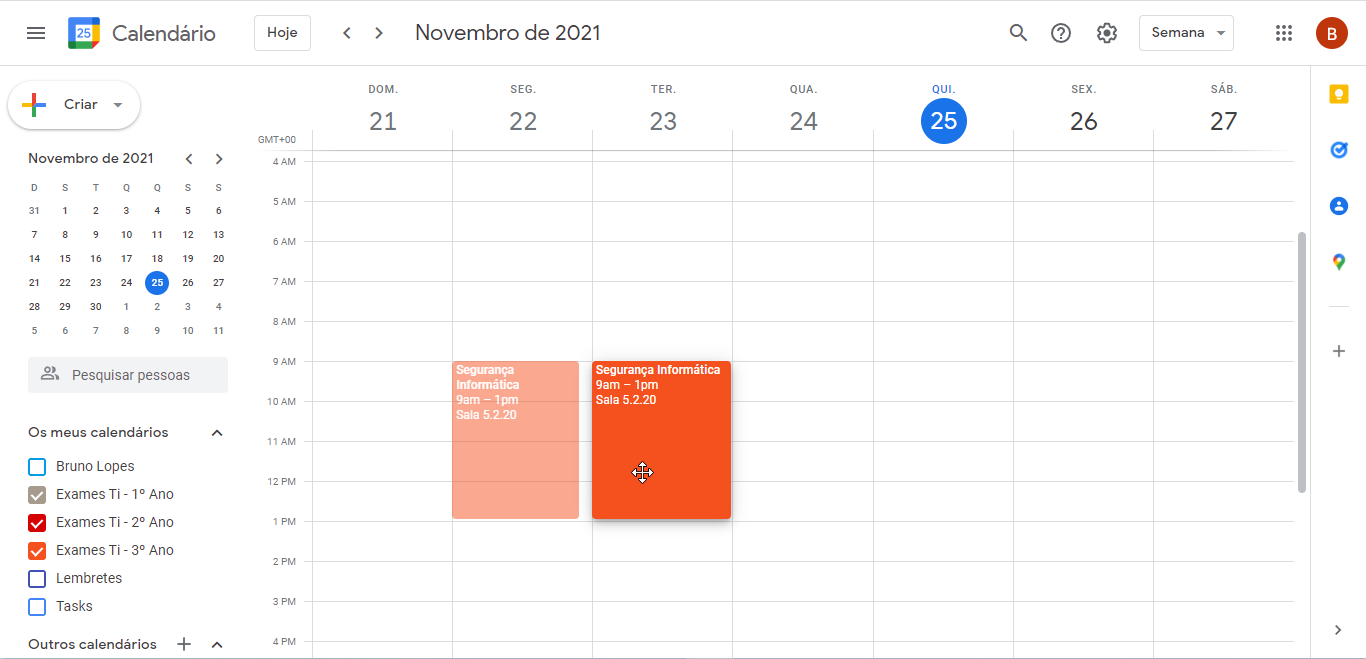
\includegraphics[width=0.8\textwidth,height=0.8\textheight,keepaspectratio]{image/estadodearte/drag_drop_google}
		\caption{Funcionalidade Drag and Drop no Google Calendar}
		\label{googledragdrop}
	\end{figure}

	\begin{figure}[H] 
		\centering
		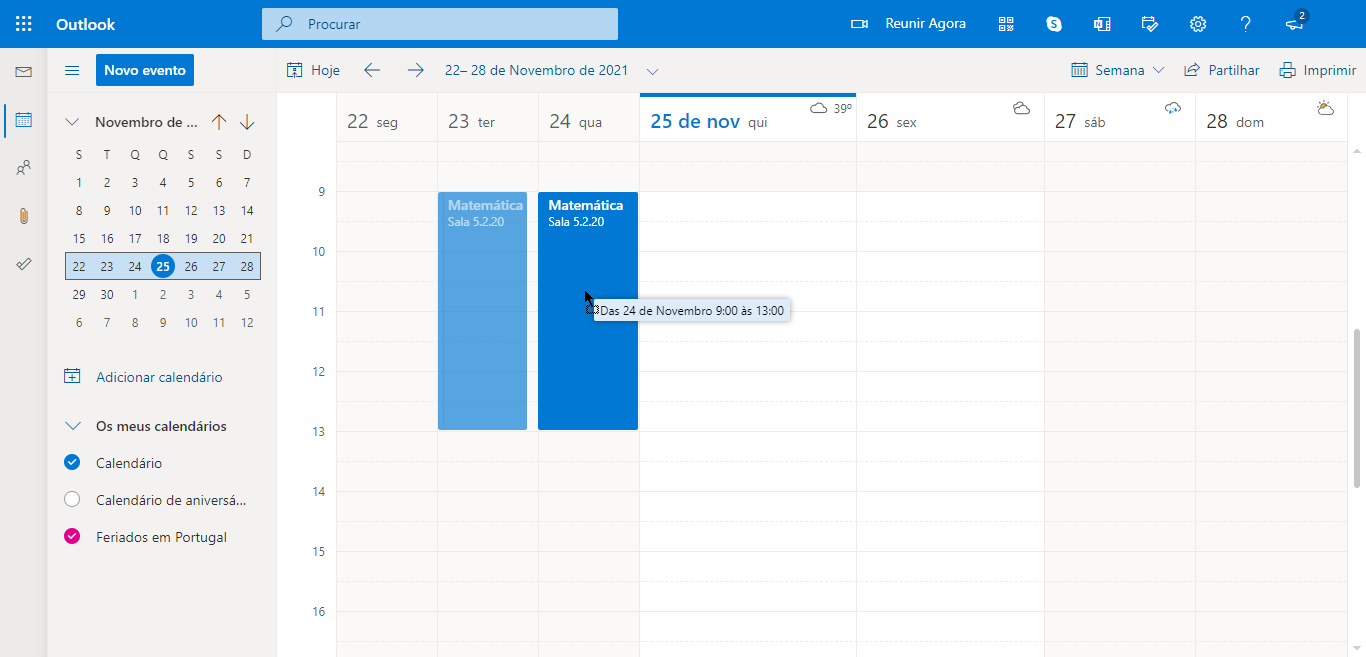
\includegraphics[width=0.8\textwidth,height=0.8\textheight,keepaspectratio]{image/estadodearte/drag_drop_outlook}
		\caption{Funcionalidade Drag and Drop no Outlook Calendar}
		\label{outlookdragdrop}
	\end{figure}

Também existe uma funcionalidade incorporada para imprimir os calendários criados, que através da funcionalidade de impressão do browser permite exportar o ficheiro numa versão .pdf, no entanto, os filtros de impressão presentes nas duas aplicações são diferentes. Ao passo que o ``Google Calendar'' que pode ser observado na figura \ref{googleexportar} permite selecionar um período de dias/semanas para imprimir, o ``Outlook Calendar'' observável na figura \ref{outlookexportar} apenas permite imprimir a semana que estamos a visualizar na aplicação, sendo necessário recorrer a esta funcionalidade múltiplas vezes caso queiramos imprimir mais do que uma semana. No entanto no ``Outlook Calendar''` é possível selecionar um período de horas para impressão, por exemplo 9h-18h, imprimindo apenas os eventos que se encontram inseridos naquele período.
	 
	\begin{figure}[H] 
		\centering
		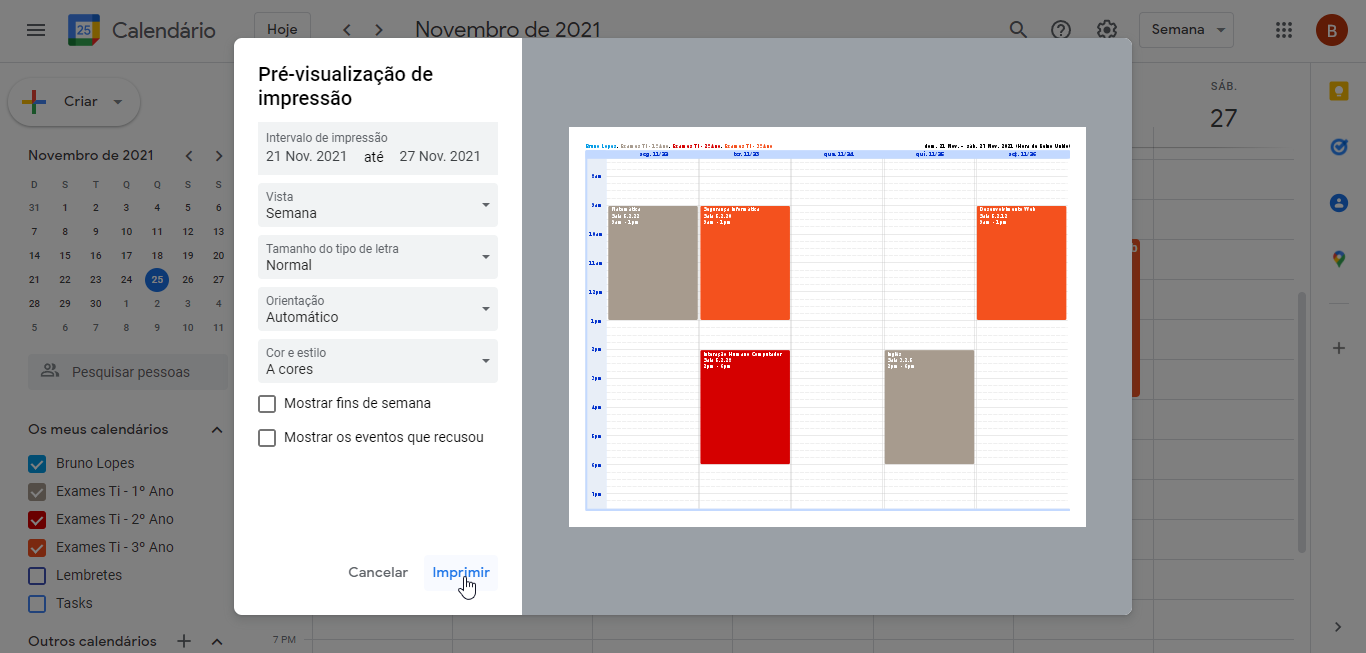
\includegraphics[width=0.8\textwidth,height=0.8\textheight,keepaspectratio]{image/estadodearte/imprimir_google}
		\caption{Funcionalidade de impressão no Google Calendar}
		\label{googleexportar}
	\end{figure}

	\begin{figure}[H] 
		\centering
		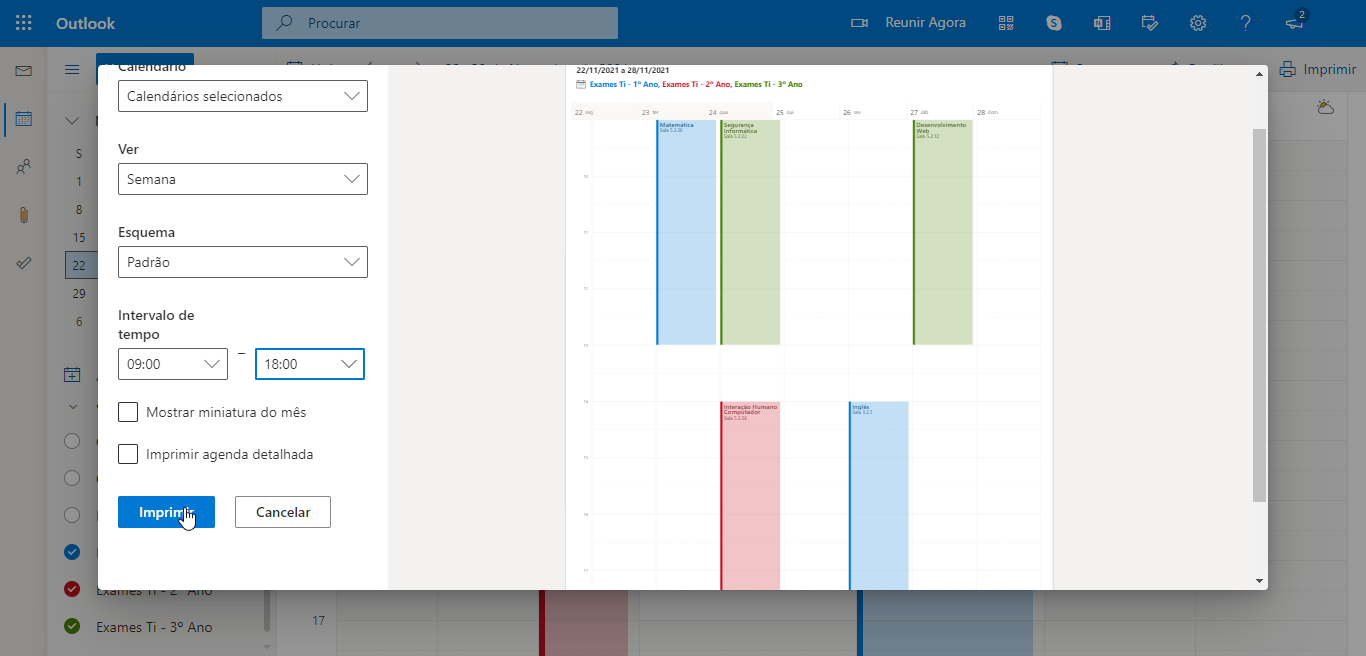
\includegraphics[width=0.8\textwidth,height=0.8\textheight,keepaspectratio]{image/estadodearte/imprimir_outlook}
		\caption{Funcionalidade de impressão no Outlook Calendar}
		\label{outlookexportar}
	\end{figure}
	
	\chapter{Tecnologias utilizadas}
	\chapter{Planificação do projeto}

 	Por consequência do âmbito do projeto este já está dividido em várias fases sendo que nesta versão do relatório só está apresentada a primeira e a segunda fase.
 	
 	Na primeira fase iniciou-se com o levantamento do estado de arte (secção \ref{estadodearte}), a reunião com o cliente (secção \ref{analiseutilizador}) e o levantamento de requisitos (secção \ref{requisitos}). Com estas informações  avançou-se para a segunda fase que consiste na prototipagem de baixa fidelidade - wireframes - e os testes com potenciais utilizadores, como se pode ver na figura \ref{cronogramaexecutado}.
		
	\clearpage
	\begin{landscape}
		\pagestyle{empty}
		
		\begin{figure}[H] 
			\centering 			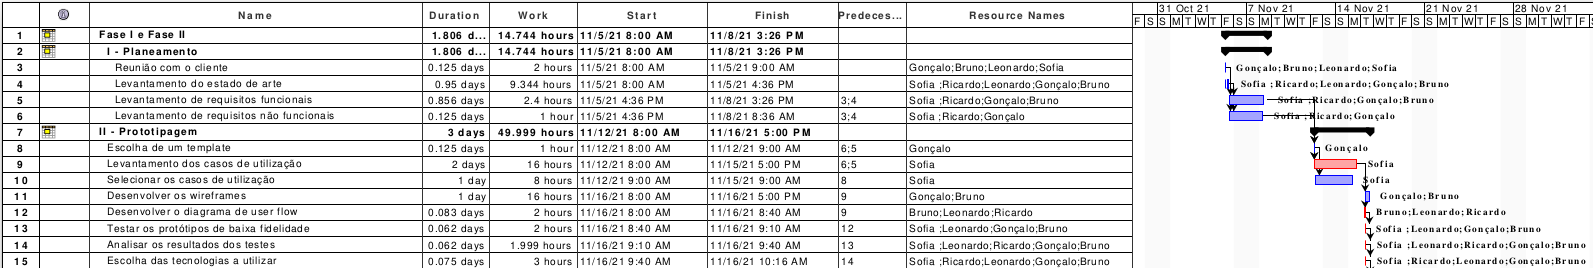
\includegraphics[width=1.4\textwidth,height=1.4\textheight,keepaspectratio]{image/planeamento_1fase}
			\caption{Planeamento da primeira e segunda fase}
			
		\end{figure}
	
	\begin{figure}[H] 
		\centering 			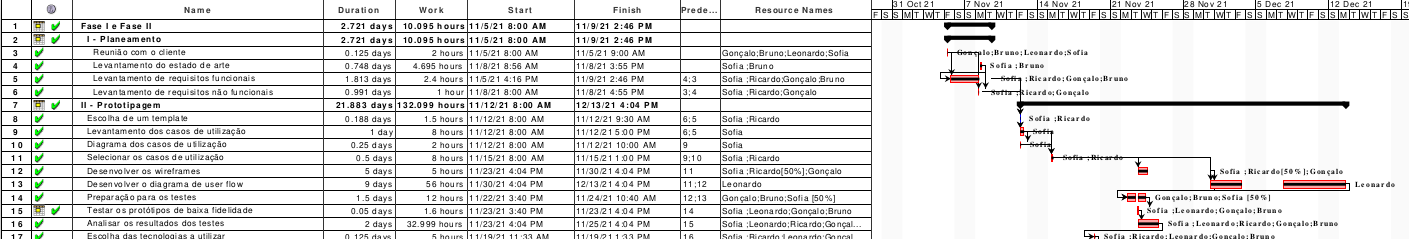
\includegraphics[width=1.4\textwidth,height=1.4\textheight,keepaspectratio]{image/cronogramaexecutado}
		\caption{Cronograma executado da primeira e segunda fase}
		\label{cronogramaexecutado}
	\end{figure}
	\end{landscape}


	
	
	\chapter{Análises dos utilizadores e tarefas}
	\label{analiseutilizador}
	
	Após a primeira reunião com o cliente chegou-se à conclusão que  este é também um potencial utilizador e que tem uma ideia precisa das funcionalidades da aplicação. Por isso, aliado à restrição de tempo achou-se que não se iria aprofundar na análise dos utilizadores. 
	
	O cliente no momento recorre ao excel para a criação de calendários,  colocando todas as salas, cursos e docentes manualmente tendo o proceso um alto risco de erro e baixa eficiência. Para além disso a formatação final (em .pdf) é exportado a partir do mesmo programa, como se pode verificar na figura \ref{calendarioatual}. Para a verificação da disponibilidade dos docentes recorre a outro programa que mostra, em forma de calendário semanal, a vermelho a indisponibilidade e a roxo quando o mesmo tem aulas, tal como está apresentado na figura \ref{disponibilidadedocentes}. 
	
	\begin{figure}[H] 
		\centering 
		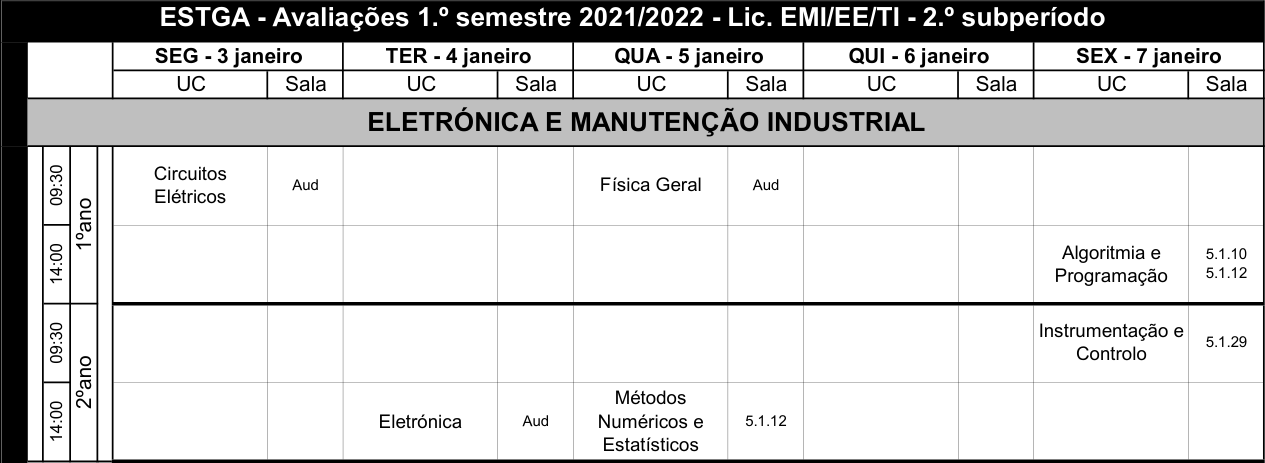
\includegraphics[width=0.7\textwidth,height=0.7\textheight,keepaspectratio]{image/calendarioavaliacao}
		\caption{Exemplo de um calendário de avaliações que é disponibilizado aos alunos}
		\label{calendarioatual}
	\end{figure}

	\begin{figure}[H] 
		\centering 
		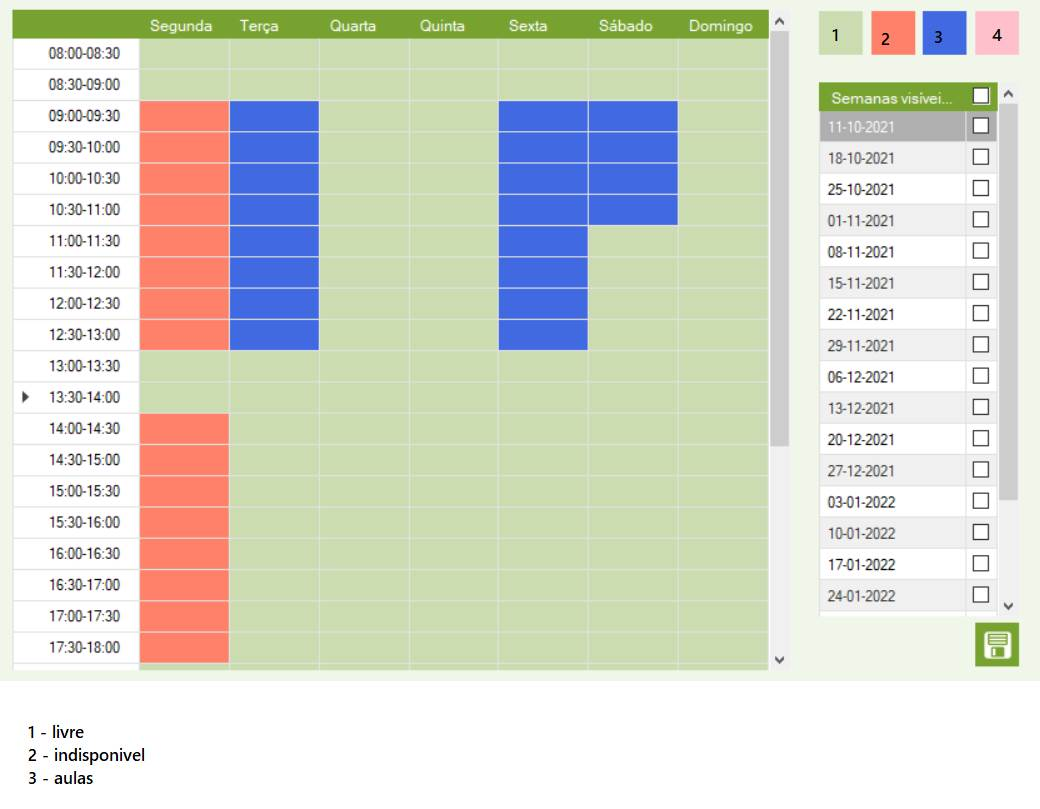
\includegraphics[width=0.7\textwidth,height=0.7\textheight,keepaspectratio]{image/ColorMap}
		\caption{Interface do programa para vizualizar a disponibilidade dos docentes}
		\label{disponibilidadedocentes}
	\end{figure}
	

	Assim, para este projeto, o cliente quer poder vizualizar todas estas informações numa só aplicação de uma forma mais eficiente e intuitiva. As informações sobre os cursos, disciplinas, docentes e salas serão importadas a partir de um ficheiro .csv que será renovado a cada semestre podendo o utilizador importar quantas vezes quiser na aplicação, atualizando todos os dados. No entanto se o ficheiro .csv conter algum erro ou faltar informação poderá alterar/inserir dentro da aplicação. Com isto o utilizador poderá criar os seus calendários associados a um ano letivo, semestre, curso e época (terá de adicionar um nome, uma data de início e fim) que criou. Apóes isso poderá marcar os exames referentes ao curso na época escolhida. Para cada exame poderá escolher um ou mais vigilantes, sendo por padrão o docente como vigilante e uma ou mais salas. No entanto caso haja alguma incongruência aparecerá um aviso a indicar qual o problema não restringindo nenhuma funcionalidade. Por fim todos os calendários criados anteriormente noutros anos letivos serão guardados num histórico, no entanto não poderá fazer quaisquer alterações.
	
	\chapter{Modelo de requisitos}
	\label{requisitos}
	\section{Requisitos funcionais}
	
	
	Os requisitos funcionais representam todas as funcionalidades que o sistema pode fazer ou que o utilizador pode realizar no sistema. Com isso na tabela \ref{requisitiosfuncionais} estam todos os requisitos funcionais dividos por várias categorias: importação, exportação, marcação de exames, configurações, avisos, autenticação, criação de calendários e histórico. Dentro da categoria ``avisos" tem as funcionalidades que o sistema irá realizar após uma ação do utilizador, ao contrário de todas as outras categorias em que o utilizador tem a possibilidade realizar determinada tarefa.
	
	Para além disso os requisitos funcionais estam classificados por prioridade sendo os de alta prioridade realizados nas primeiro e os de baixa prioridade implementados por último, tal como está listado na secção \ref{selecaocasosdeuso}.  
	
	
	
\def\arraystretch{1.5}
	\begin{center}
		\label{requisitiosfuncionais}
		\begin{longtable}{|m{1cm}|m{2.2cm}|m{10cm}|m{2cm}|}
			\caption{Requisitos funcionais}\\
			
			\hline			
			\textbf{Refª }	& \textbf{Categoria}&\textbf{Descrição do requisito} & \textbf{Prioridade} \\
			\hline
			
			
			RF.1 &Importação& Importação de ficheiros com a configuração de salas, disciplinas e docentes em formato .csv & Alta \\
			\hline
			
			RF.2 &\multirow{2}{2cm}{Exportação}& Exportação de calendários em formato .pdf & Alta \\
			
			RF.3 && Exportação o calendário em língua inglesa & Baixa \\
			\hline
			
			RF.4 &\multirow{3}{2cm}{Marcação de exames}& Os exames podem ser marcados em três turnos: às 9h30, às 14h e às 18h30 & Alta \\
			
			RF.5 && Associação de um ou mais vigilantes a cada exame & Alta \\
			
			RF.6 && O calendário não deverá permitir a marcação de exames aos domingos e feriados & Alta \\
			
			RF.7 &&	Associação de uma ou mais salas a cada exame & Alta\\
			
			RF.8 && Se houver vários cursos com o mesmo exame então será associado a todos os calendários dos cursos associados. & Média\\
			\hline
		
			RF.9 &\multirow{7}{2cm}{Configurações}& Configuração do tipo de sala (informática, laboratório de redes e normal) e lotação máxima & Alta \\
			
			RF.10 & & Inserção de cursos e disciplinas & Alta\\
			
			RF.11 && Permitir inserir novos docentes & Alta\\
			
			RF.12 && Permitir editar informações (nome, que disciplinas está a lecionar, horário de trabalho) sobre os docentes & Alta\\
			
			RF.13 && Permitir editar informações (nome do curso, docente e a disciplina) sobre as disciplinas e cursos & Alta\\
			
			RF.14 && Alterar a disponibilidade dos docentes & Alta\\
			
			RF.15 && Permitir colocar restrições arbitrárias introduzidas pelo utilizador & Baixa \\
			\hline	
			
			RF.16 &\multirow{9}{2cm}{Avisos}& Aparecimento de um aviso no caso de incongruência da informação durante a marcação de exames & Alta \\
			
			RF.17 &&Mostrar um aviso de alta prioridade se houver sobreposições de exames & Alta\\
			
			RF.18 && Mostrar um aviso de alta prioridade se o docente não estiver disponível & Alta \\
			
			RF.19 && Mostrar um aviso de alta prioridade se a sala não estiver disponível & Alta\\
			
			RF.20 && Mostrar um aviso de alta prioridade se o curso for diurno e colocar um exame no turno da noite e vice-versa & Média\\
			
			RF.21&&Mostrar um aviso de alta prioridade se o docente associado ao mesmo exame for repetido & Alta \\
			
			RF.22 && Mostrar um aviso de alta prioridade se o exame necessitar de uma sala de informática e não for associada sala desse tipo & Média\\
			
			RF.23 && Mostrar um aviso de alta prioridade se houver mais alunos inscritos do que  lotação máxima da sala & Alta\\
			
			RF.24 && Mostrar um aviso de média prioridade se houver exames marcados no mesmo dia e hora do mesmo curso mas anos diferentes & Média\\
			
			
			RF.25 && Mostrar um aviso de média prioridade se o utilizador tentar exportar um calendário sem exames marcados & Média\\
			\hline
			
			RF.26 &Autenticação& O utilizador só pode aceder à aplicação após a autenticação & Alta\\
			\hline
			
			RF.27 &\multirow{3}{2cm}{Criação de calendários}&Criação de calendários associados a um curso, ano letivo, ano do curso, época e semestre.& Alta \\
			
			RF.28 && Criação de épocas de avaliação adicionando um nome e uma data de início e fim & Alta \\
			
			RF.29 && A criação de um novo calendário deverá sempre partir do início sem exames marcados & Alta\\
			\hline
			RF.30 &\multirow{2}{*}{Histórico}& Guardar e visualizar calendários de exames de anos anteriores (histórico)& Média \\
			
			RF.31 && Filtrar o histórico por curso, ano letivo, ano do curso, semestre e época& Média \\
			\hline
		\end{longtable}
	\end{center}



	
	\section{Requisitos não funcionais}
	
	Os requisitos não funcionais estão dividos em três categorias: requsitos de interface e facilidade de uso que representam todos os requisitos que melhorem a usabilidade da aplicação; requisitos de segurança e integridade dos dados e requisitos de interface com sistemas externos e ambientes de execução.
	
	\subsection{Requisitos de interface e facilidade de uso}

Assim que o utilizador inicia a sessão na aplicação este tem de facilmente entender como a aplicação está organizada. Isto permite que o utilizador utilize a aplicação durante mais tempo e gerir os calendários de avaliaçõesnão seja frustrante.
	
	\begin{table}[H]
	\caption{Requisitos de interface e facilidade de uso}
	
	\begin{center}
		\begin{tabularx}{\textwidth}{|c|X|c|}
			\hline
			\textbf{Refª }	& \textbf{Descrição do requisito} & \textbf{Prioridade} \\
			\hline
			RIF1 & As disciplinas e cursos podem ser inseridas através de \textit{drag e drop} &Alta\\
			\hline
			RIF2 & Interface responsiva permitindo a sua visualização em ambiente mobile &Alta\\
			\hline
			RIF3 & Linguagem padrão em Português de Portugal &Alta\\
			\hline
			RIF4 & Há dois tipos de avisos distinguidos com texto e cor &Alta\\
			\hline
		\end{tabularx}
		\label{requisitosdeinterface}
	\end{center}
	\end{table}

	\subsection{Requisitos de segurança e integridade dos dados}
	
	Para que o utilizador possa colocar os seus dados na aplicação sem conter risco de transvazar para utilizadores indesejados foram criados alguns requisitos de segurança referido na	tabela \ref{requisitosdeseguranca}.
	
\begin{table}[H]	
	\caption{Requisitos de segurança e integridade dos dados}
	
	
	\begin{center}
		\begin{tabularx}{\textwidth}{|c|X|c|}
			\hline
			\textbf{Refª }	& \textbf{Descrição do requisito} & \textbf{Prioridade} \\
			\hline
			RSI1 &O histórico não pode ter associações a outras tabelas da base de dados  &Alta\\
			\hline
			RSI2 & Uma única conta de utilizador&Alta\\
			\hline
		\end{tabularx}
		\label{requisitosdeseguranca}
	\end{center}
\end{table}


	\subsection{Requisitos de interface com sistemas externos e ambientes de execução}
	
	A aplicação por ambiente da disciplina irá ser programada em linguagens web,
	consequentemente não é necessário definir que sistema operativos pode a aplicação ser executada.
	No entanto é crucial ter acesso à rede da Universidade de Aveiro e um dos navegadores definidos na tabela \ref{requisitosdesistemas}.
	
	\def\arraystretch{1.5}
	\begin{table}[H]
		\caption{Requisitos de interface com sistemas externos e ambientes de execução}
		\begin{center}
			\begin{tabularx}{\textwidth}{|c|X|c|}
				\hline
				\textbf{Refª }	& \textbf{Descrição do requisito} & \textbf{Prioridade}\\
				\hline
				RSA1 & Suportar Browsers com motor renderização webkit/blink (Chrome, Edge, Safari, Brave, etc.)  & Alta \\
				\hline
				RSA2 & Suportar Firefox ESR e outros derivados de gecko/quantum & Alta \\
				\hline
				RSA5 & Estar conectado à rede da Universidade de Aveiro & Alta\\
				\hline
			\end{tabularx}
			\label{requisitosdesistemas}
		\end{center}
	\end{table}
		
	
	\chapter{Modelo de casos de utilização}
	
	
	Para entender quais são as funcionalidades da aplicação e como irá interagir com o utilizador foi criado um modelo de casos de utilização apartir do estado de arte (ver secção \ref{estadodearte}), da análise dos utilizadores e tarefas  (ver secção \ref{analiseutilizador}) e dos requisitos funcionais (ver secção \ref{requisitos}). Este é composto pelo diagrama de casos de utilização (ver figura \ref{usecasediagram}) e pela descrição dos mesmos, que são detalhadas ao nível da interação do utilizador com a aplicação (ver secção \ref{descricaousecase}). Neste modelo só existe um ator que tem acesso a todas as funcionalidades da aplicação. 
	Para ajudar na prototipagem da aplicação os casos de utilização foram divididos em várias fases consoante a prioridade dos requsitos funcionais associados (ver secção \ref{selecaocasosdeuso}).
	
	\section{Diagrama de casos de utilização}
	\label{diagrama}
	
	No diagrama apresentado na figura \ref{usecasediagram} tem só um único ator que é o utilizador que tem acesso a todas as funcionalidades mas para as realizar terá de iniciar sessão. A seguir terá de importar dados a partir de um ficheiro ou inserir-los na aplicação, caso a aplicação não tenha dados do semestre atual. Caso exista algum erro ou queira atualizar alguma informação pode alterar dados sobre as salas e a sua lotação máxima, docentes, cursos e disciplinas. Com isto pode criar calendários e marcar os seus exames associando vigilantes e salas aos exames. Contudo se enganar nas datas de início e fim poderá corrigir durante a criação. Para além disso caso haja alguma incronguência, durante a marcação de exames, a aplicação irá mostrar um aviso consoante o seu tipo. Após a criação de calendários pode vê-los através do histórico podendo filtrá-los por curso, ano, época, ano do curso e por semestre. Por fim pode exportar para pdf em português ou em inglês todos os calendários que pretender.
	
	No entanto todos estes casos de utilização estam com uma explicação mais detalhada na secção \ref{descricaousecase}.
	
	
\clearpage
\begin{landscape}
	\pagestyle{empty}
	
		\begin{figure}[H] 
			\centering 			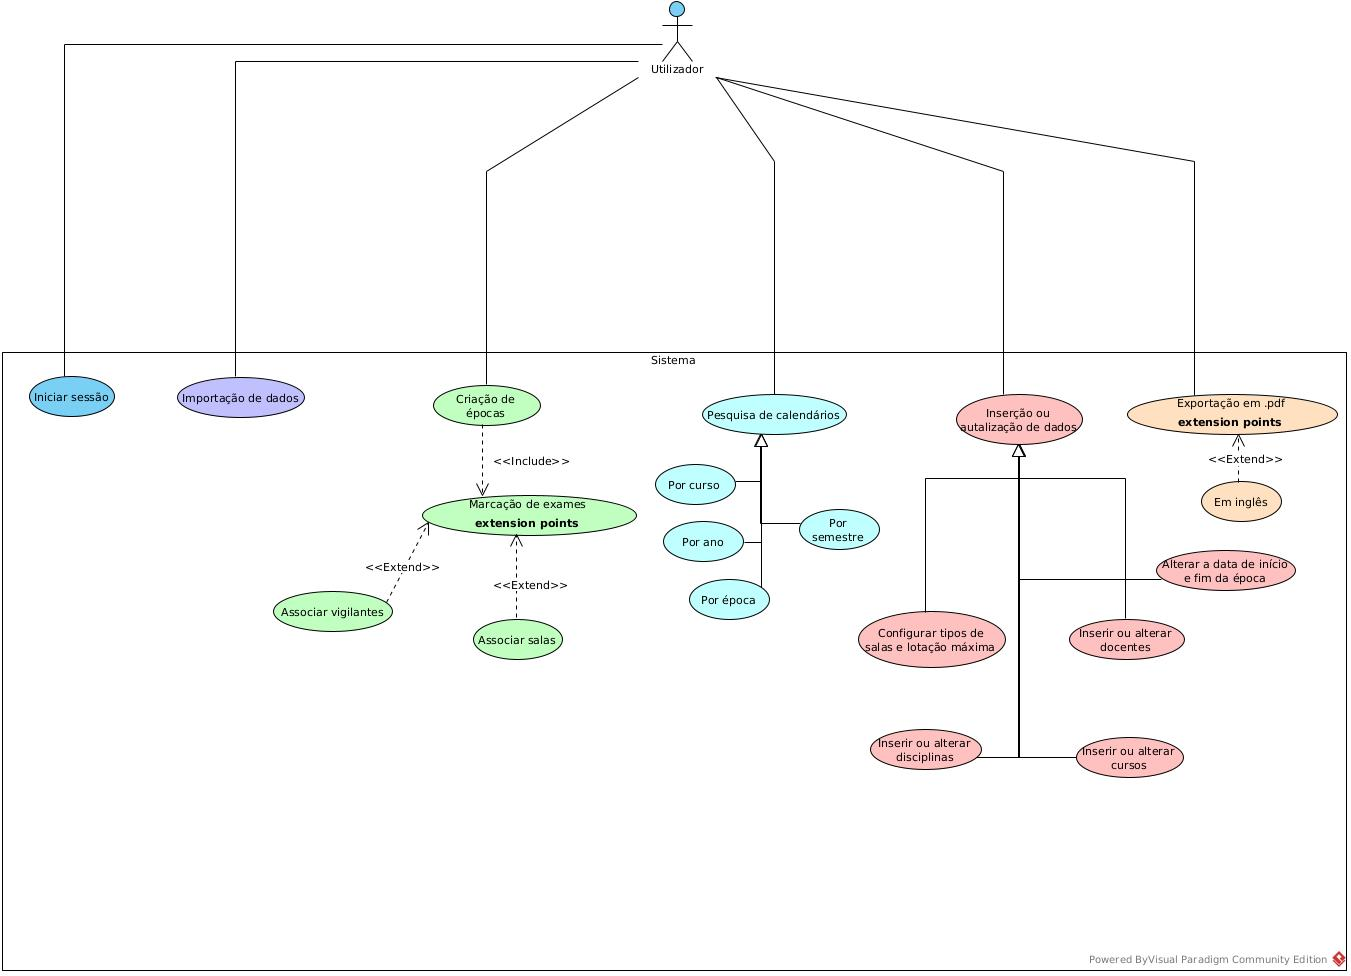
\includegraphics[width=1.3\textwidth,height=1.3\textheight,keepaspectratio]{image/diagrama}
			\caption{Diagrama dos casos de utilização}
			\label{usecasediagram}
		
		\end{figure}
\end{landscape}


	\section{Seleção dos casos de utilização}
	\label{selecaocasosdeuso}
	
	Para uma maior eficiência na implementação e prototipagem dos casos de utilização estes foram divididos em várias fases consoante a sua prioridade e a sua dependência de outros casos. Assim sendo os casos de utilização da primeira fase são os mais prioritários e são a base da aplicação:
	
	\begin{itemize}
		\item Autenticação;
		\item Importação de ficheiros .csv com a configuração de salas, disciplinas e docentes;
	 	\item Criação de calendários com época, curso, ano letivo, semestre e ano do curso associado.
	 	\item Marcação de exames no calendário.
	 	\item Inserção de vigilantes e salas nos exames marcados;
	\end{itemize}
	
	Os casos de utilização da segunda fase dependem dos casos de utilização da primeira fase no entanto também são de alta prioridade: 
	
	\begin{itemize}
		\item Vizualização do histórico de calendários filtrando-os por curso, ano letivo, semestre, época e ano do curso.
		\item Inserção e alteração de cursos e disciplinas a partir da interface;
		\item Inserção e alteração de novos docentes;
		\item Exportação do calendário em formato pdf;
	\end{itemize}


	Na terceira fase contém os avisos mais importantes a mostrar durante a utilização da aplição para além da configuração da disponiblidade dos docentes:
	
	\begin{itemize}
		\item Associar na área de docentes dias em que os mesmos não estão disponíveis;
		\item Avisar se houver sobreposição de exames;
		\item Avisar se o docente não estiver disponível;
		\item Avisar se houver mais alunos inscritos do que a lotação máxima da sala;
		\item Avisar se a sala não estiver disponível;
		\item Avisar caso o docente associado ao exame for repetido;
	\end{itemize}
	
	Por último, na quarta fase, contém todos os casos de utilização de média e baixa prioridade:
	\begin{itemize}
		\item Avisar se o curso for diurno e houver uma marcação para o turno das 18h30 e vice-versa.
		\item Associar o mesmo exame a todos os cursos que têm a mesma disiplina.
		\item Avisar caso o tipo de sala associada ao exame não for apropriada (informática ou normal)
		\item Exportação do calendário em inglês
	\end{itemize}

	
	\section{Descrição dos casos de utilização}
	\label{descricaousecase}
	
	Para complementar o diagrama de casos de utilização (ver secção \ref{diagrama}) estes foram descritos detalhamente com através dos seguintes parâmetros: ator, prioridade, requisitos funcionais associados, finalidade, pré-condições, interação e cenários alternativo. Os cenários alternativos consistem em outras interações que o utilizador possa ter, para além da principal, e qual a sua interação e reação da aplicação. Para além disso para uma melhor compreensão tem alguns wireframes associados a cada caso de utilização.
	
	\def\arraystretch{1.5}
	\begin{table}[H]
		\caption{Caso de utilização - autenticação}
		\begin{center}	
			\begin{tabularx}{\textwidth}{|l|X|}
				\hline
				\textbf{Nome }	& \textbf{Autenticação} \\
				\hline
				Atores: & Utilizador \\
				\hline
				Prioridade: & Alta \\
				\hline
				Requisitos funcionais:& RF.25\\
				\hline
				Finalidade: & Aceder às funcionalidades da aplicação\\
				\hline
				Sumário: & Com o seu email e palavra-passe o utilizador pode aceder às funcionalidades da aplicação.\\
				\hline
				Pré-condições: & Estar conectado à rede da Universidade de Aveiro.\\
				\hline
				Descrição da interação: &  O utilizador assim que abre a aplicação tem de iniciar a sessão com o seu email e palavra-passe correspondentes.\\
				\hline
				Cenário alternativo 1:& \textbf{Esqueceu da palavra-passe:} Poderá criar uma nova através do botão "Esqueceu-se da palavra-passe".\\
				\hline
			\end{tabularx}
		\end{center}
	\end{table}

	\begin{figure}[H] 
		\centering 
		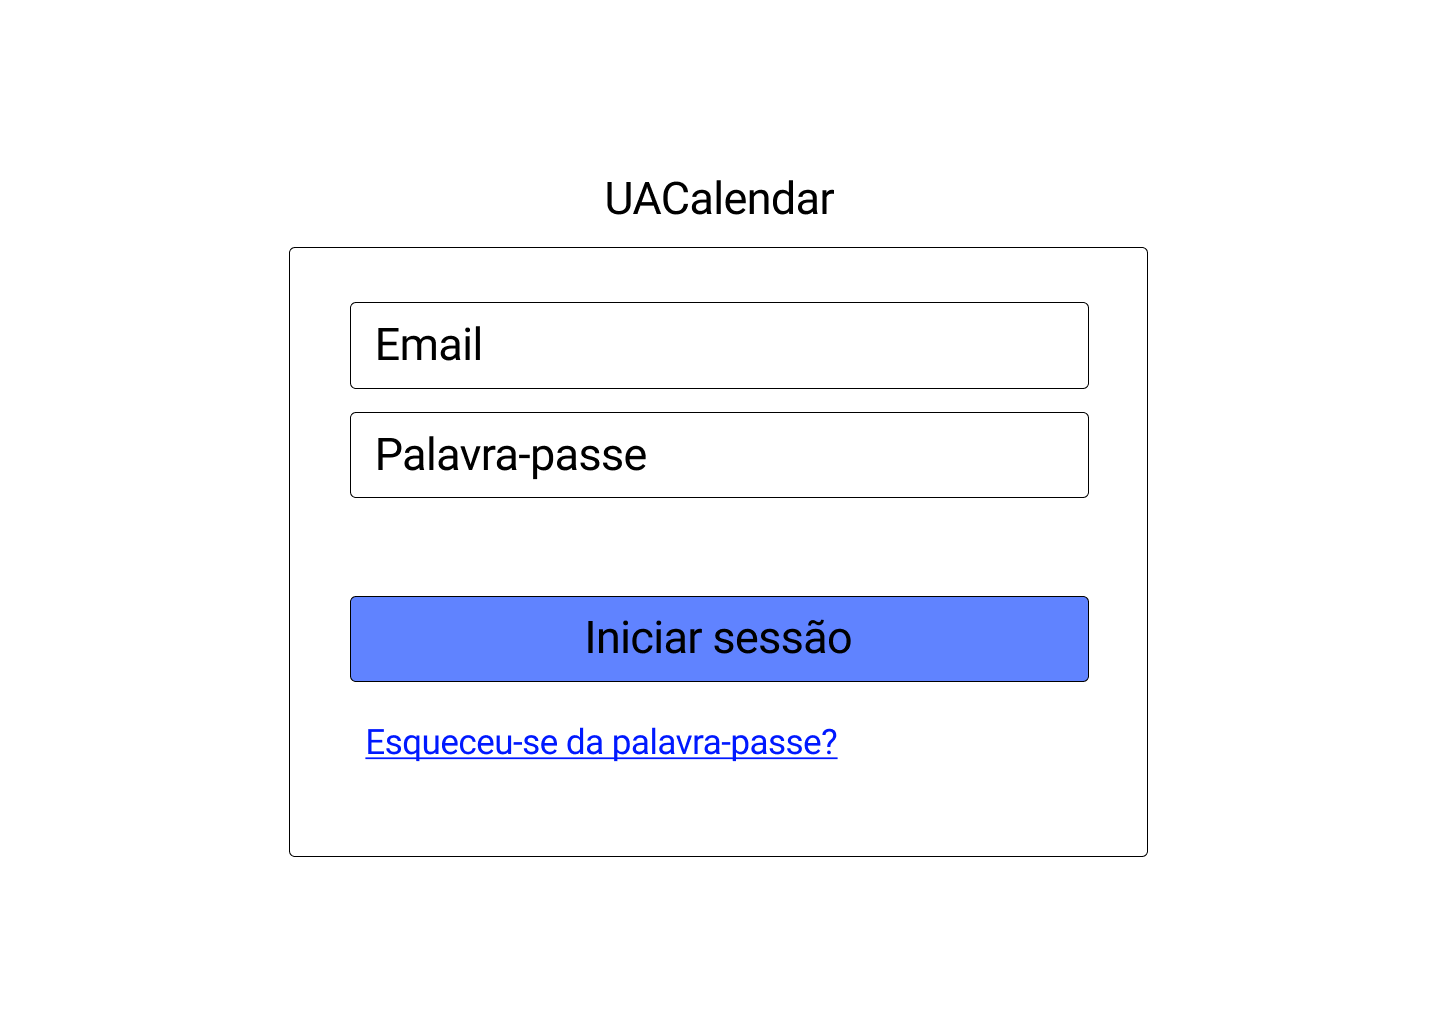
\includegraphics[width=0.7\textwidth,height=0.7\textheight,keepaspectratio]{image/prototipowireframes/autenticacao}
		\caption{Interface para o utilizador iniciar sessão.}
		\label{usecaseautenticacao}
	\end{figure}

\def\arraystretch{1.5}
\begin{table}[H]
	\caption{Caso de utilização - importação de ficheiros .csv}
	\label{usecaseimportarcsv}
	\begin{center}	
		\begin{tabularx}{\textwidth}{|l|X|}
			\hline
			\textbf{Nome }	& \textbf{Importação de ficheiros .csv} \\
			\hline
			Atores: & Utilizador\\
			\hline
			Prioridade: &  Alta\\
			\hline
			Requisitos funcionais:&  RF.1, RF.26\\
			\hline
			Finalidade: & Obter e guardar todos os dados referentes aos docentes, cursos e salas. \\
			\hline
			Sumário: & O utilizador pode importar ficheiros no formato .csv que contenha informações sobre os docentes, salas, cursos e disciplinas para que possa criar calendários (ver tabela \ref{usecasecriarcalendario})\\
			\hline
			Pré-condições: & Ter iniciado sessão na aplicação.\\
			\hline
			Descrição da interação:& Antes da criação do primeiro calendário do semestre corrente o utilizador tem de importar um ficheiro no formato .csv para a obtenção de todos os dados, como se pode ver na figura \ref{avisoimportarcsv} e na figura \ref{importarcsv}. No entanto caso já tenha importado anteriormente o utilizaodor pode prosseguir diretamente para a criação de calendários.\\
			\hline
			Cenário alternativo 1: &\textbf{O ficheiro contém erros de formatação:} Aparecerá um aviso a indicar que não é possível o ficheiro em questão porque contém erros. Terá de corrigir e de seguida tente novamente. Volta para a página de importação.\\
			\hline
			Cenário alternativo 2: &\textbf{O ficheiro tem informações em falta:} Aparecerá um aviso indicando que contém informações em falta mas que pode adicionar nas configurações.\\
			\hline
			Cenário alternativo 3: &\textbf{O ficheiro escolhido não é do formato .csv:} Será rejeitado a sua importação e aparecerá um ficheiro a informar que o ficheiro não é do formato .csv.\\
			\hline
			Cenário alternativo 4: &\textbf{O ficheiro escolhido não tem a informação esperada:} Será rejeitado a sua importação e aparecerá um ficheiro a informar que o ficheiro contém informações sobre os cursos, salas e/ou docentes\\
			\hline
		\end{tabularx}
	\end{center}
\end{table}



\begin{figure}[H] 
	\centering 
	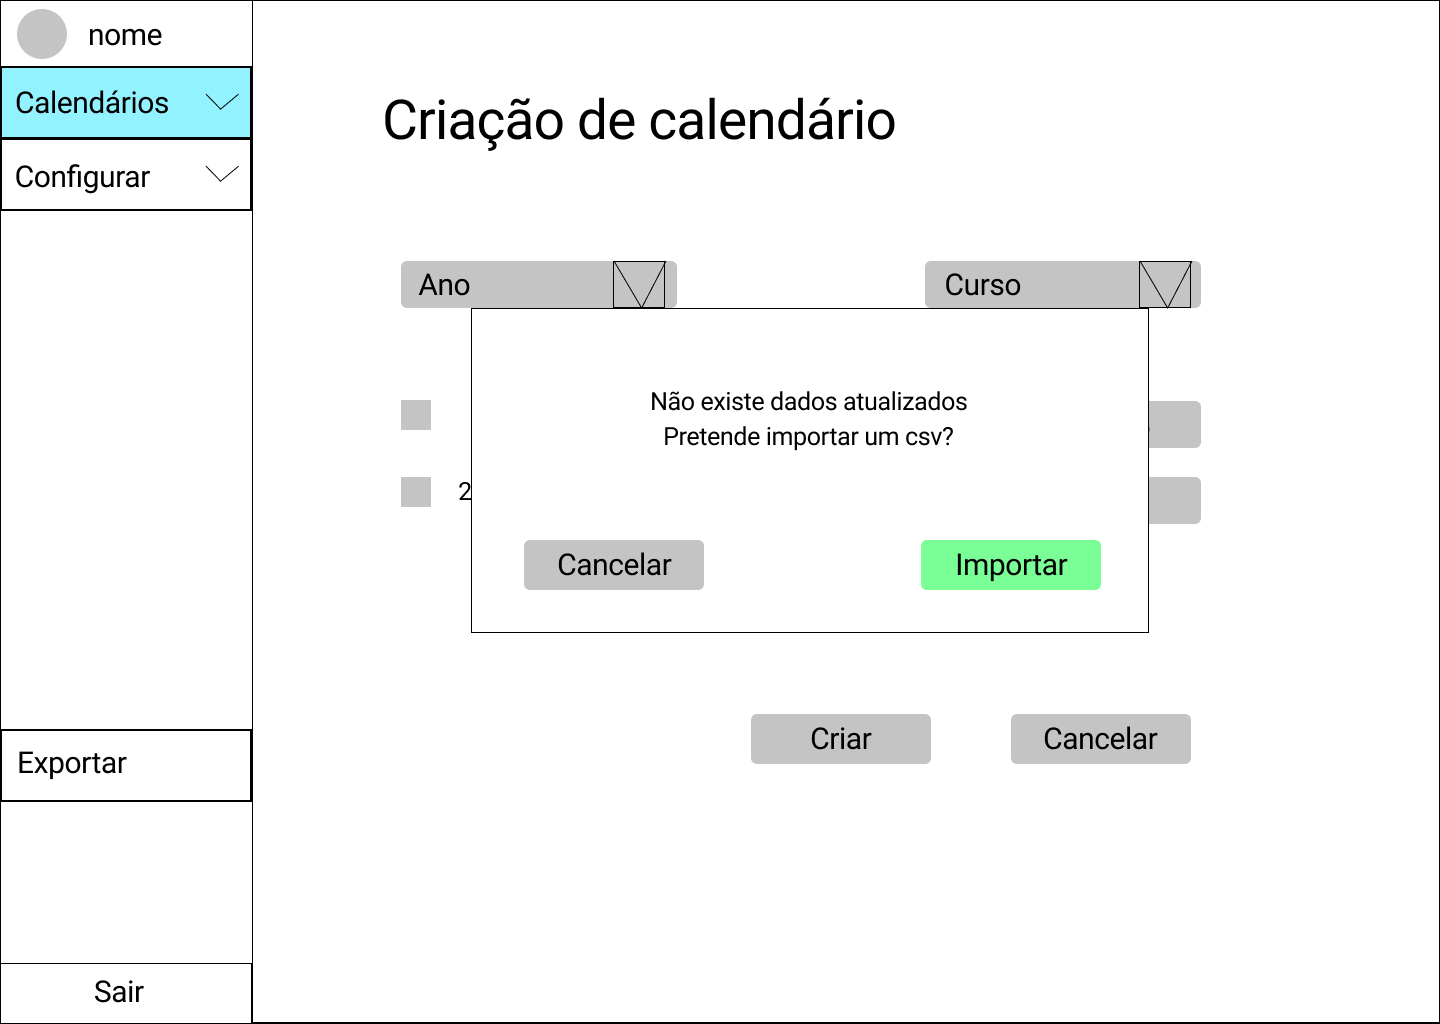
\includegraphics[width=0.8\textwidth,height=0.8\textheight,keepaspectratio]{image/prototipowireframes/criarCalendariosAviso}
	\caption{Aviso que não existe dados referentes ao semestre corrente}
	\label{avisoimportarcsv}
\end{figure}


\begin{figure}[H] 
	\centering 
	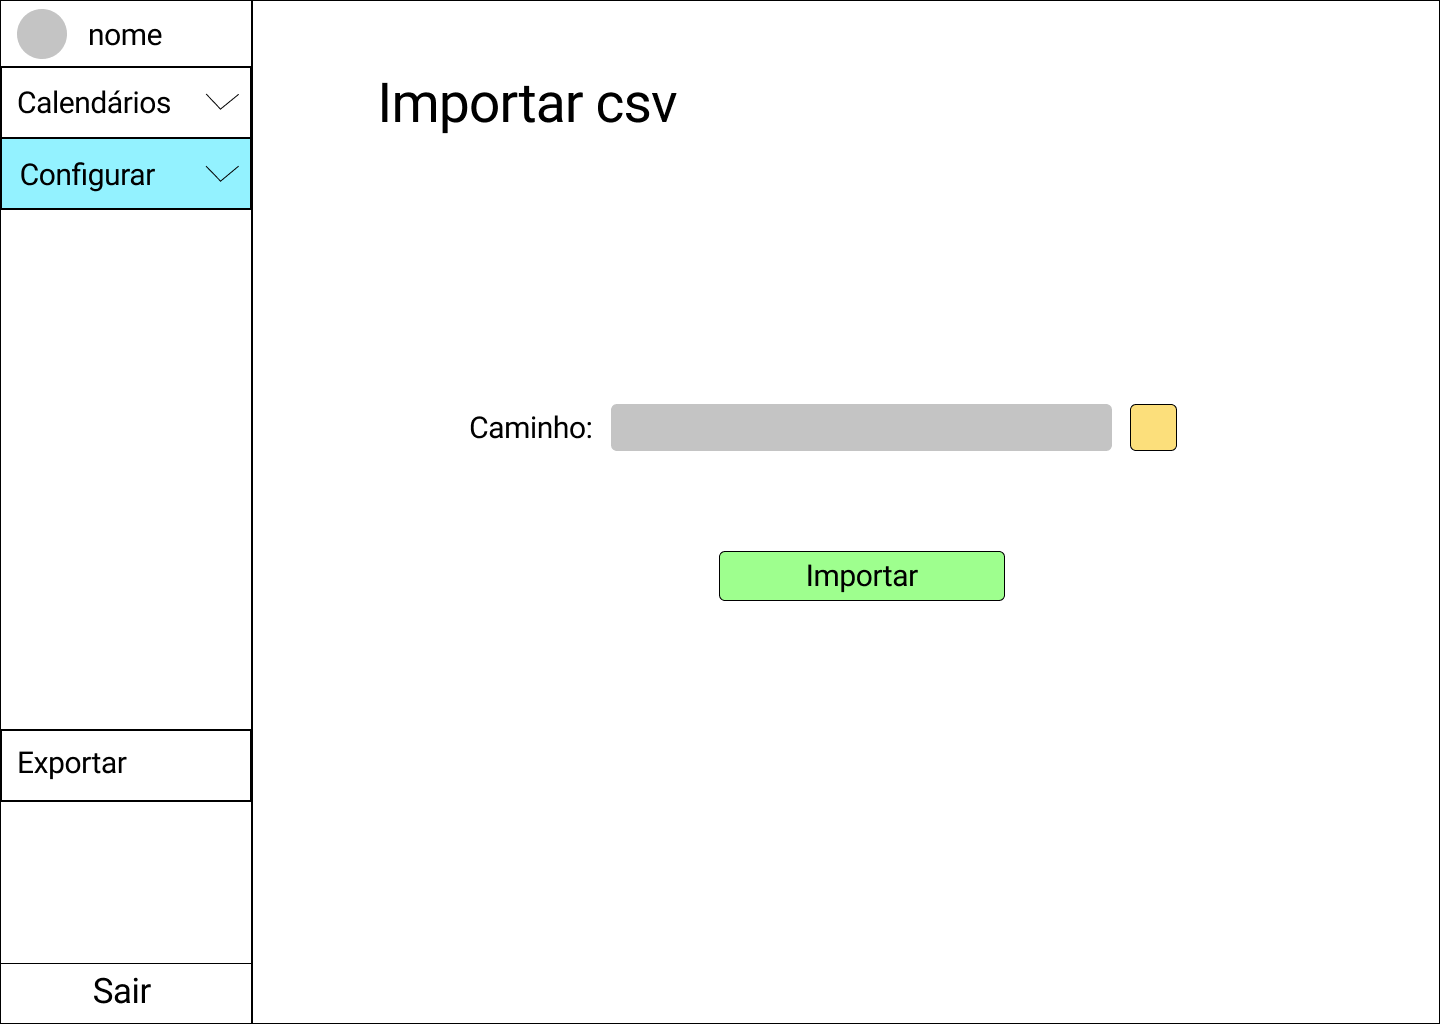
\includegraphics[width=0.8\textwidth,height=0.8\textheight,keepaspectratio]{image/prototipowireframes/importar}
	\caption{Interface para importar ficheiros em formato .csv}
	\label{importarcsv}
\end{figure}



\def\arraystretch{1.5}
\begin{table}[H]
	\caption{Caso de utilização - criação de um calendário}
	\label{usecasecriarcalendario}
	\begin{center}	
		\begin{tabularx}{\textwidth}{|l|X|}
			\hline
			\textbf{Nome: }	& \textbf{Criação de um calendário} \\
			\hline
			Ator(es): & Utilizador\\
			\hline
			Prioridade: &  Alta\\
			\hline
			Requisitos funcionais:& RF.1, RF.26, RF.27, RF.28, RF.29\\
			\hline
			Finalidade: & Criação de um novo calendário de avaliação\\
			\hline
			Sumário: & O utilizador pode criar um calendário associando o curso, o ano do curso, o ano letivo, a época (nome, data de início e fim) e o semestre.\\
			\hline
			Pré-condições: & Ter iniciado sessão na aplicação, ter importado ou adicionado informações sobre os cursos, disciplinas, docentes e salas.\\
			\hline
			Descrição da interação: & O utilizador para criar um novo calendário terá de clicar em ``novo'' na figura \ref{interfacevercalendario}. Depois terá de preencher todos os campos (ver figura \ref{interfacecriarcalendario}): curso, ano do curso, ano letivo, nome da época e a sua data de início e fim. Por fim clica no botão ``criar". \\
			\hline
			Cenário alternativo 1: &\textbf{Não preenche todos os campos  expostos:} Aparecerá uma mensgem de aviso que terá de preencher todos os campos para a criação de um novo calendário.\\
			\hline
			Cenário alternativo 2: &\textbf{Quer cancelar a ação:} Clica no botão ``cancelar" e nenhuma informação será guardada.\\
			\hline
			Cenário alternativo 3: &\textbf{Não existe dados sobre os curso, cursos e/ou docentes:} Pergunta se quer importar um ficheiro .csv (ver figura \ref{avisoimportarcsv})\\
			\hline
		\end{tabularx}
	\end{center}
\end{table}


\begin{figure}[H] 
	\centering 
	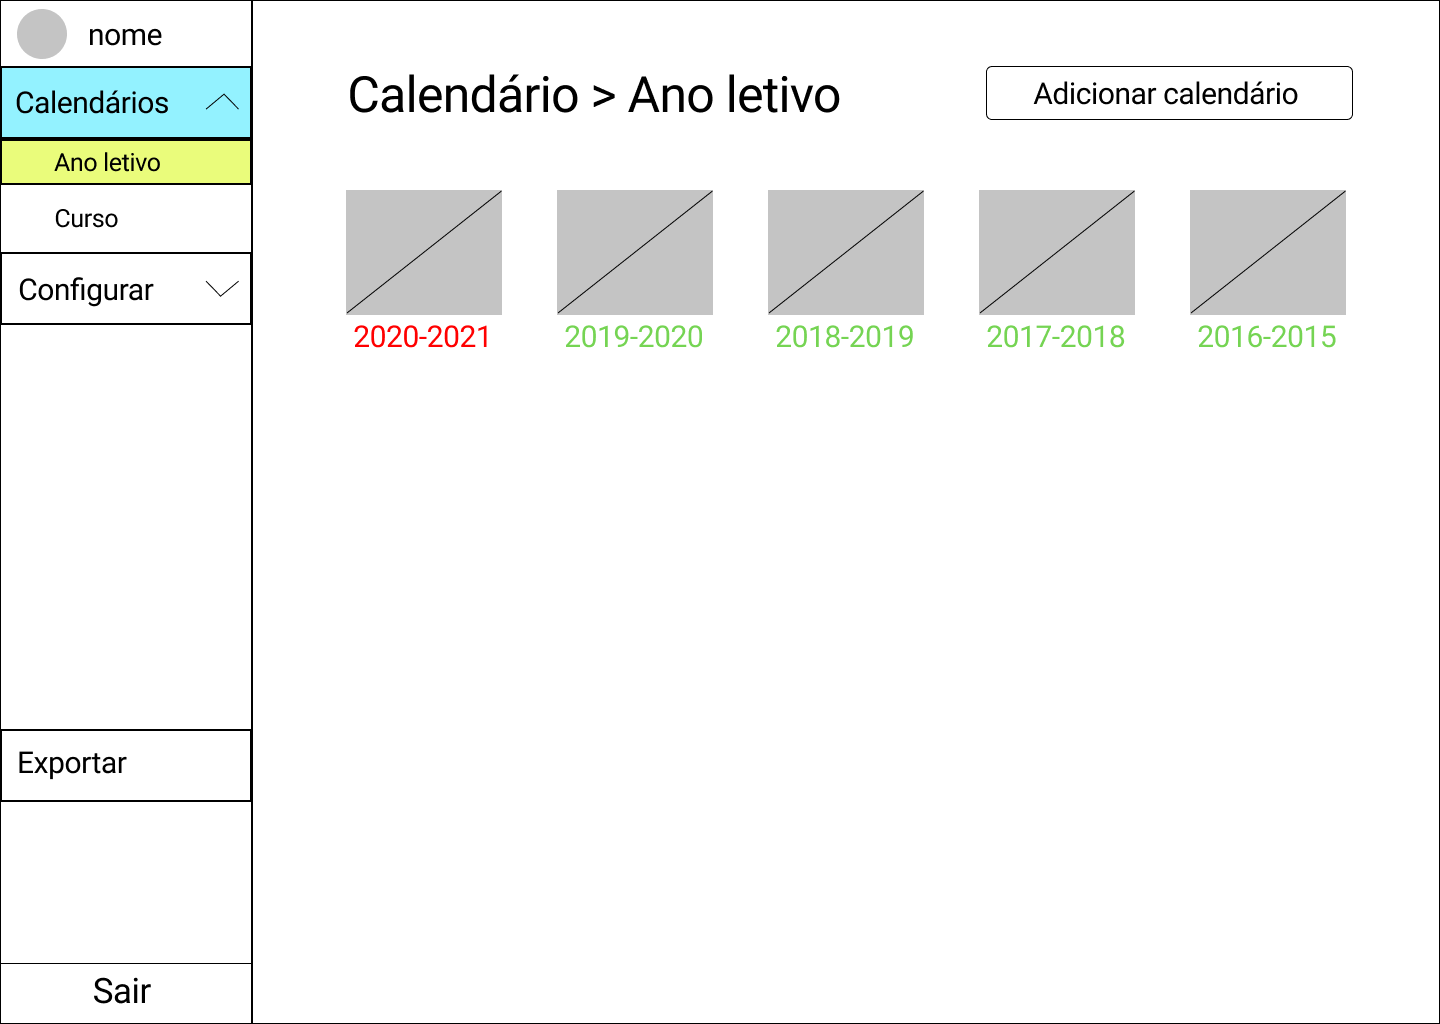
\includegraphics[width=0.8\textwidth,height=0.8\textheight,keepaspectratio]{image/prototipowireframes/pesquisacalendarioanoletivo}
	\caption{Interface para visualizar o histórico de calendários}
	\label{interfacevercalendario}
\end{figure}

\begin{figure}[H] 
	\centering 
	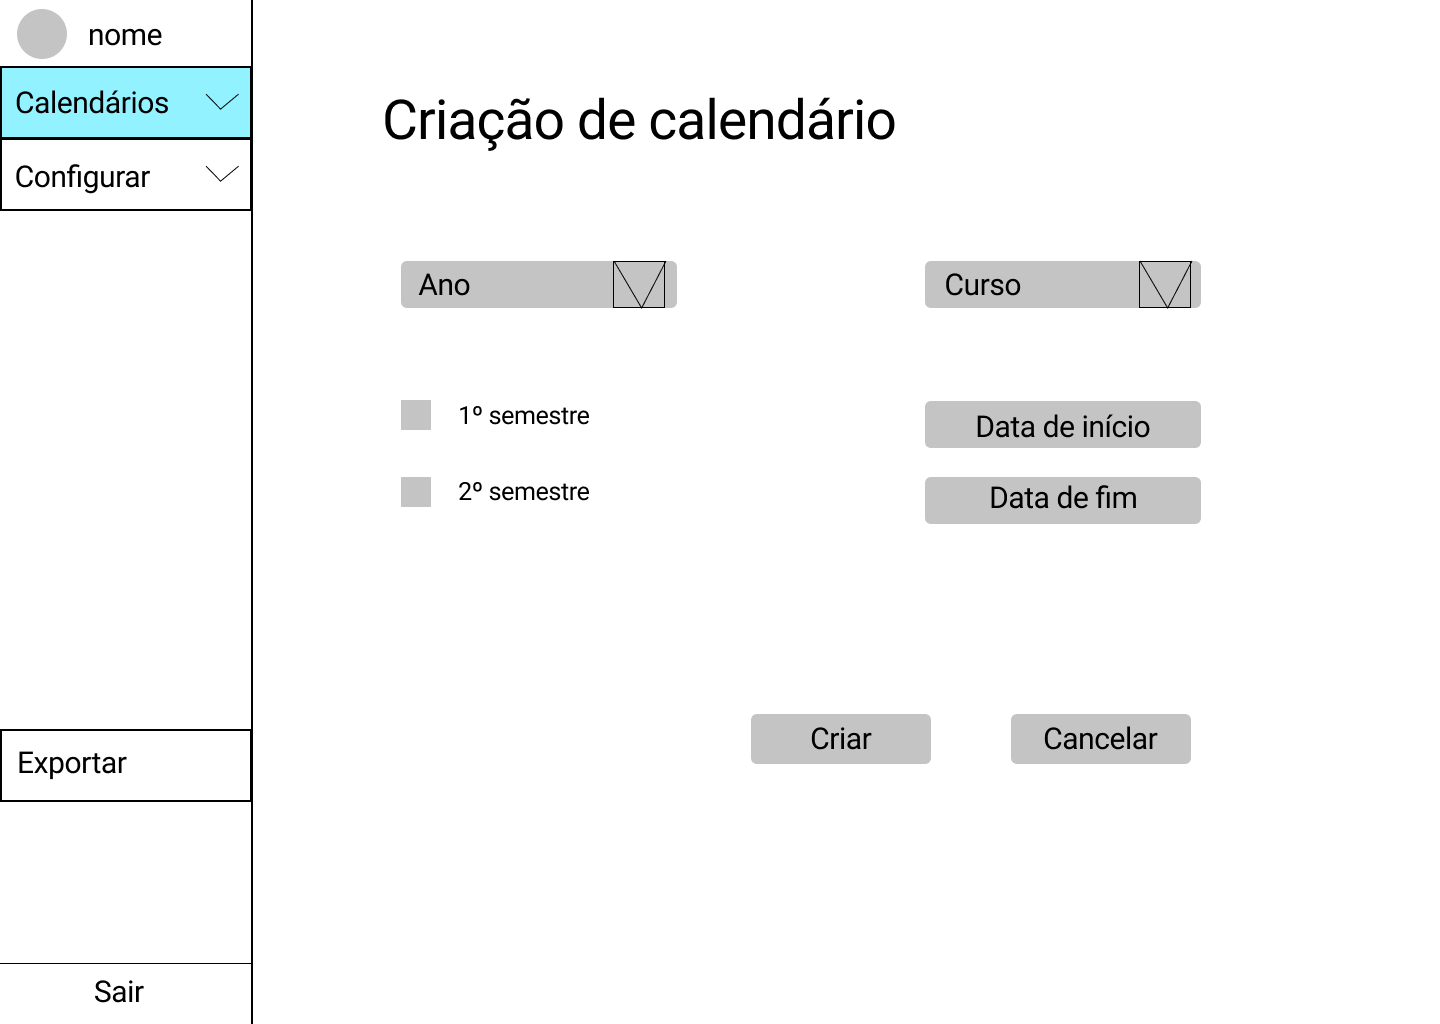
\includegraphics[width=0.8\textwidth,height=0.8\textheight,keepaspectratio]{image/prototipowireframes/criarcalendario}
	\caption{Interface para a criação de novos calendários}
	\label{interfacecriarcalendario}
\end{figure}
	

\def\arraystretch{1.5}
\begin{center}
	\label{usecasemarcarexame}
	\begin{longtable}{|m{4cm}|m{12cm}|}
		\caption{Caso de utilização - marcação de exames no calendário}\\
		
			\hline
		\textbf{Nome }	& \textbf{Marcação de exames no calendário} \\
		\hline
		Atores: & Utilizador\\
		\hline
		Prioridade: &  Alta\\
		\hline
		Requisitos funcionais:&  RF.1, RF.4, RF.5, RF.6, RF.7, RF.8\\
		\hline
		Finalidade: & Marcação de exames na época de avaliações\\
		\hline
		Sumário: & O utilizador pode marcar os exames no calendário criado (ver caso de utilização na tabela \ref{usecasecriarcalendario}). Pode marcar num dos três horários: 9h30, 14h e 18h30.\\
		\hline
		Pré-condições: & Ter iniciado sessão na aplicação, ter importado ou adicionado informações sobre os cursos, disciplinas, docentes e salas e ter criado um novo calendário.\\
		\hline
		Descrição da interação: & O utilizador terá todas as disciplinas do curso (e ano do curso) escolhido na lista do lado esquerdo (ver figura \ref{interfacemarcarexame}), em relação ao calendário , em que poderá marcar exame em qualquer um dos três horários: 9h30, 14h e 18h30. Assim que marcar um exame a disciplina associada desaparece da lista. Por fim pode adicionar mais vigilantes (tendo o docente como primeiro vigilante) e uma ou mais salas.  \\
		\hline
		Cenário alternativo 1: & \textbf{Marca um exame no mesmo dia e na mesma hora que outro exame anteriormente marcado:} Aparece um aviso de alta prioridade a informar que existe sobreposição de exames\\
		\hline
		
		
		Cenário alternativo 2: & \textbf{Marca um exame se marcar um exame no horário das 18h30 e o curso é diurno e vice-versa:} Aparece um aviso de alta prioridade a informar que o exame marcado está fora do horário do curso\\
		\hline
		
		Cenário alternativo 3: & \textbf{Existe sobreposição de exames no mesmo curso mas anos diferentes:} Aparece um aviso de média prioridade a informar que existe sobreposição de exames em anos diferentes do mesmo curso\\
		\hline
	\end{longtable}
\end{center}


	\begin{figure}[H] 
		\centering 
		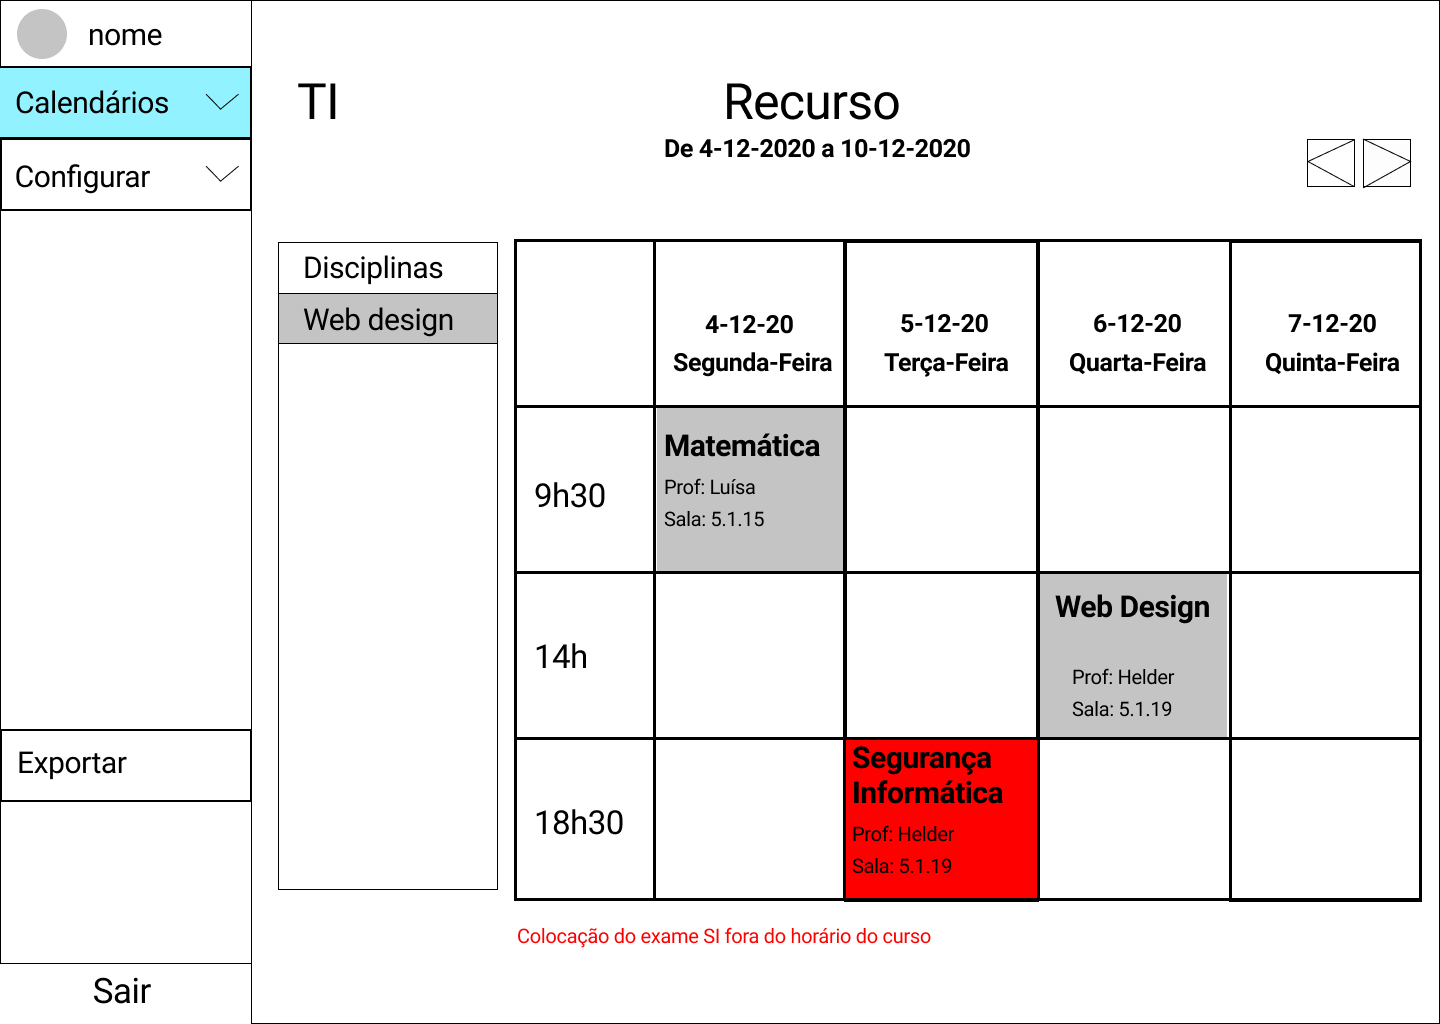
\includegraphics[width=0.8\textwidth,height=0.8\textheight,keepaspectratio]{image/prototipowireframes/calendarioaviso}
		\caption{Interface para marcação de exames no calendário}
		\label{interfacemarcarexame}
	\end{figure}


	
\def\arraystretch{1.5}
\begin{center}
	\begin{longtable}{|m{4cm}|m{12cm}|}
	\caption{Caso de utilização - inserção de vigilantes e salas nos exames marcados}\\
		
		\hline
	\textbf{Nome }	& \textbf{Inserção de vigilantes e salas nos exames marcados} \\
	\hline
	Atores: & Utilizador\\
	\hline
	Prioridade: &  Alta\\
	\hline
	Requisitos funcionais:& RF.1, RF.5, RF.7, RF.26 \\
	\hline
	Finalidade: & Inserção de vigilantes e salas a exames marcados.\\
	\hline
	Sumário: & O utilizador pode adicionar mais que um vigilante a um exame marcado (ver caso de utilização na tabela \ref{usecasemarcarexame}) e uma ou mais salas.\\
	\hline
	Pré-condições: & Ter iniciado sessão na aplicação, ter criado calendários de avaliação e ter marcado exames.\\
	\hline 
	Descrição da interação: & O utilizador após marcar um exame pode clicar no exame e aparecerá um pop-up (ver figura \ref{interfacevigilantes}) em que pode adicionar vigilantes (por padrão será adicionado o docente da disciplina) e uma ou mais salas. \\
	\hline
	Cenário alternativo 1: & \textbf{Associa um docente a um exame que não está disponível:} Aparece um aviso de alta prioridade a indicar que o docente associado não está disponível\\
	\hline
	Cenário alternativo 2: & \textbf{Associa uma sala a um exame que está ocupada:} Aparece um aviso de alta prioridade a indicar que o docente associado não está disponível\\
	\hline
	Cenário alternativo 3: & \textbf{Associa um docente a um exame que não está disponível:} Aparece um aviso de alta prioridade a indicar que o docente associado não está disponível\\
	\hline
	Cenário alternativo 4: & \textbf{Associa o mesmo docente ao mesmo exame duas vezes:} Aparece um aviso de alta prioridade a informar que existe um vigilante duplicado\\
	\hline
	Cenário alternativo 5: & \textbf{Associa uma sala que não é apropriada para o exame:} Aparece um aviso de alta prioridade a informar que o tipo de sala (informática, laboratório de redes ou normal) não está de acordo com o exame\\
	\hline
	Cenário alternativo 6: & \textbf{A soma da lotação total das salas associadas ao exame é inferior ao número de alunos inscritos à disciplinas:} Aparece um aviso de alta prioridade a informar que necessita de mais salas para o exame marcado\\
	\hline
	\end{longtable}
\end{center}


	\begin{figure}[H] 
	\centering 
	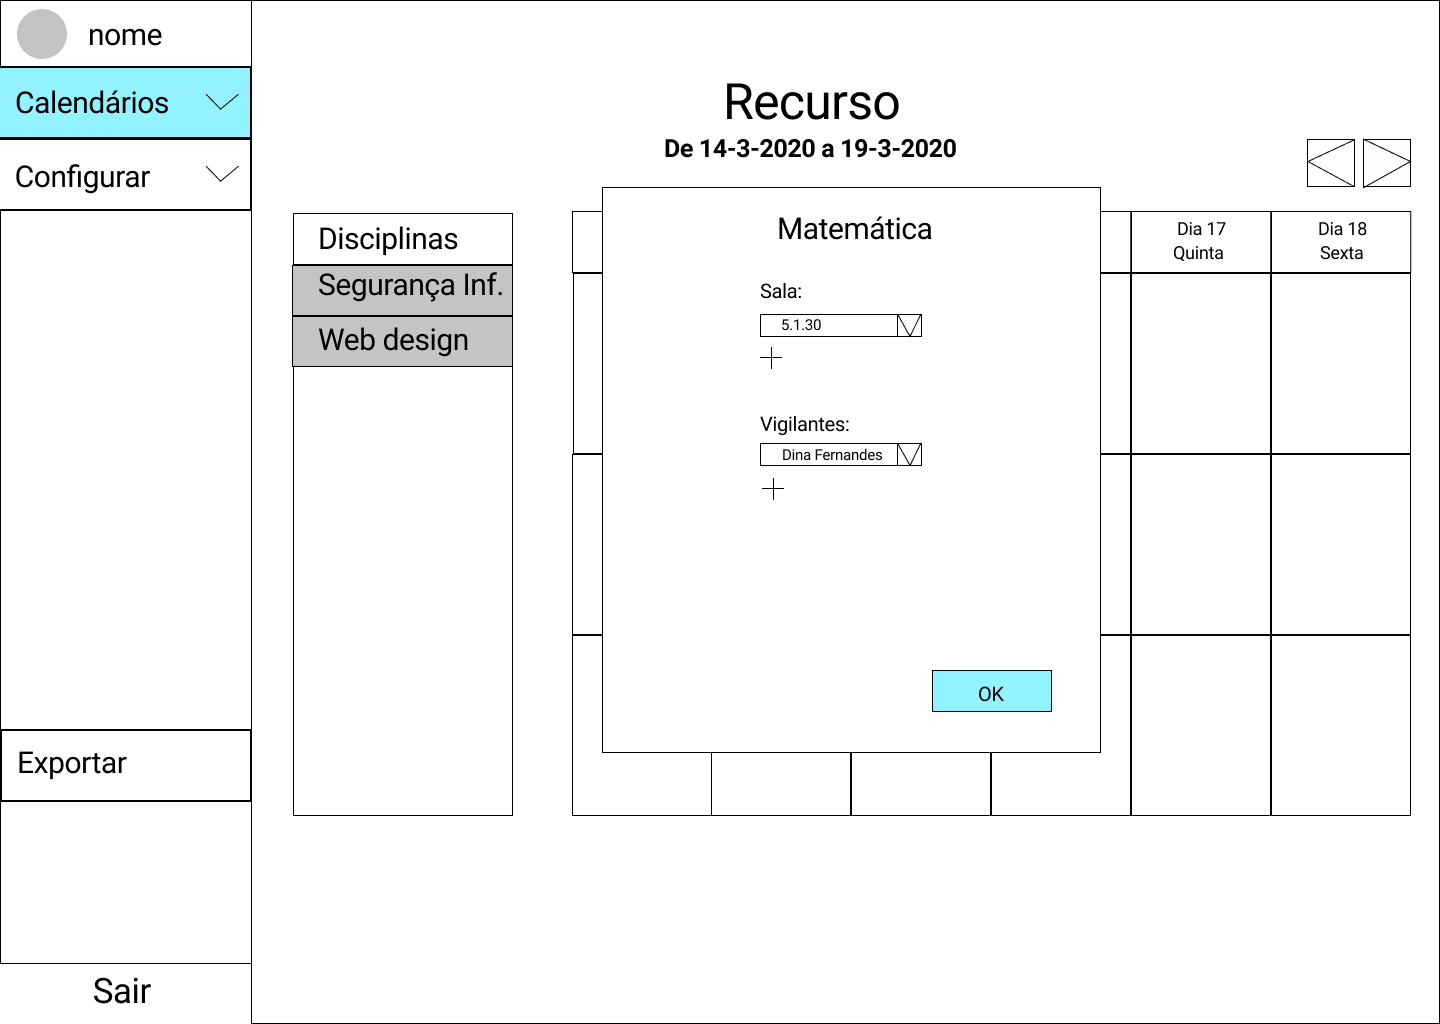
\includegraphics[width=0.8\textwidth,height=0.8\textheight,keepaspectratio]{image/prototipowireframes/popup}
	\caption{Associar vigilantes e salas a exames marcados}
	\label{interfacevigilantes}
\end{figure}

	\def\arraystretch{1.5}
\begin{table}[H]
	\caption{Caso de utilização - Inserção e alteração de dados a partir da interface}
	\begin{center}	
		\begin{tabularx}{\textwidth}{|l|X|}
			\hline
			\textbf{Nome }	& \textbf{Inserção e alteração de dados} \\
			\hline
			Atores: & Utilizador \\
			\hline
			Prioridade: & Alta \\
			\hline
			Requisitos funcionais:& RF.1, RF.9, RF.10, RF.11, RF.12, RF.13, RF.14, RF.26 \\
			\hline
			Finalidade: & Atualizar ou inserir nova informação sobre docentes, disciplinas e/ou salas.\\
			\hline
			Sumário: &  O utilizador pode inserir ou alterar informações sobre disciplinas e cursos.\\
			\hline
			Pré-condições: & Estar conectado à rede da Universidade de Aveiro e para alterar ou elimnar necessita já ter inserido dados sobre os docnetes, salas e disciplinas ou importado um ficheiro no formato .csv (ver caso de utilização na tabela \ref{usecaseimportarcsv}).\\
			\hline
			Descrição da interação: &  O utilizador ao entrar no menu ``configurar" poderá escolher entre vizualizar disciplinas, salas ou docentes. Dentro de "Disciplinas" (ver figura \ref{interfaceconfdisciplinas}) pode alterar o nome da disciplina, o docente e o curso associado. Em ``Docentes" (ver figura \ref{interfaceconfdocentes}) pode alterar o nome do docente, o seu email e os dias disponíveis. E por fim em ``Salas" (ver figura \ref{interfaceconfsalas}) poderá mudar o tipo e a lotação máxima. Em todas estas secções pode eliminar, alterar ou adicionar quantas vezes quiser.\\
			\hline
			Cenário alternativo 1:&\textbf{Quer retroceder nas alterações feitas:} O utilizador pode eliminar qualquer uma das informações apresentadas.\\
			\hline
			Cenário alternativo 2:&\textbf{Insere informação repetida:} Aparece um aviso a informação que existe informação duplicada.\\
			\hline
		\end{tabularx}
	\end{center}
\end{table}

	\begin{figure}[H] 
		\centering 
		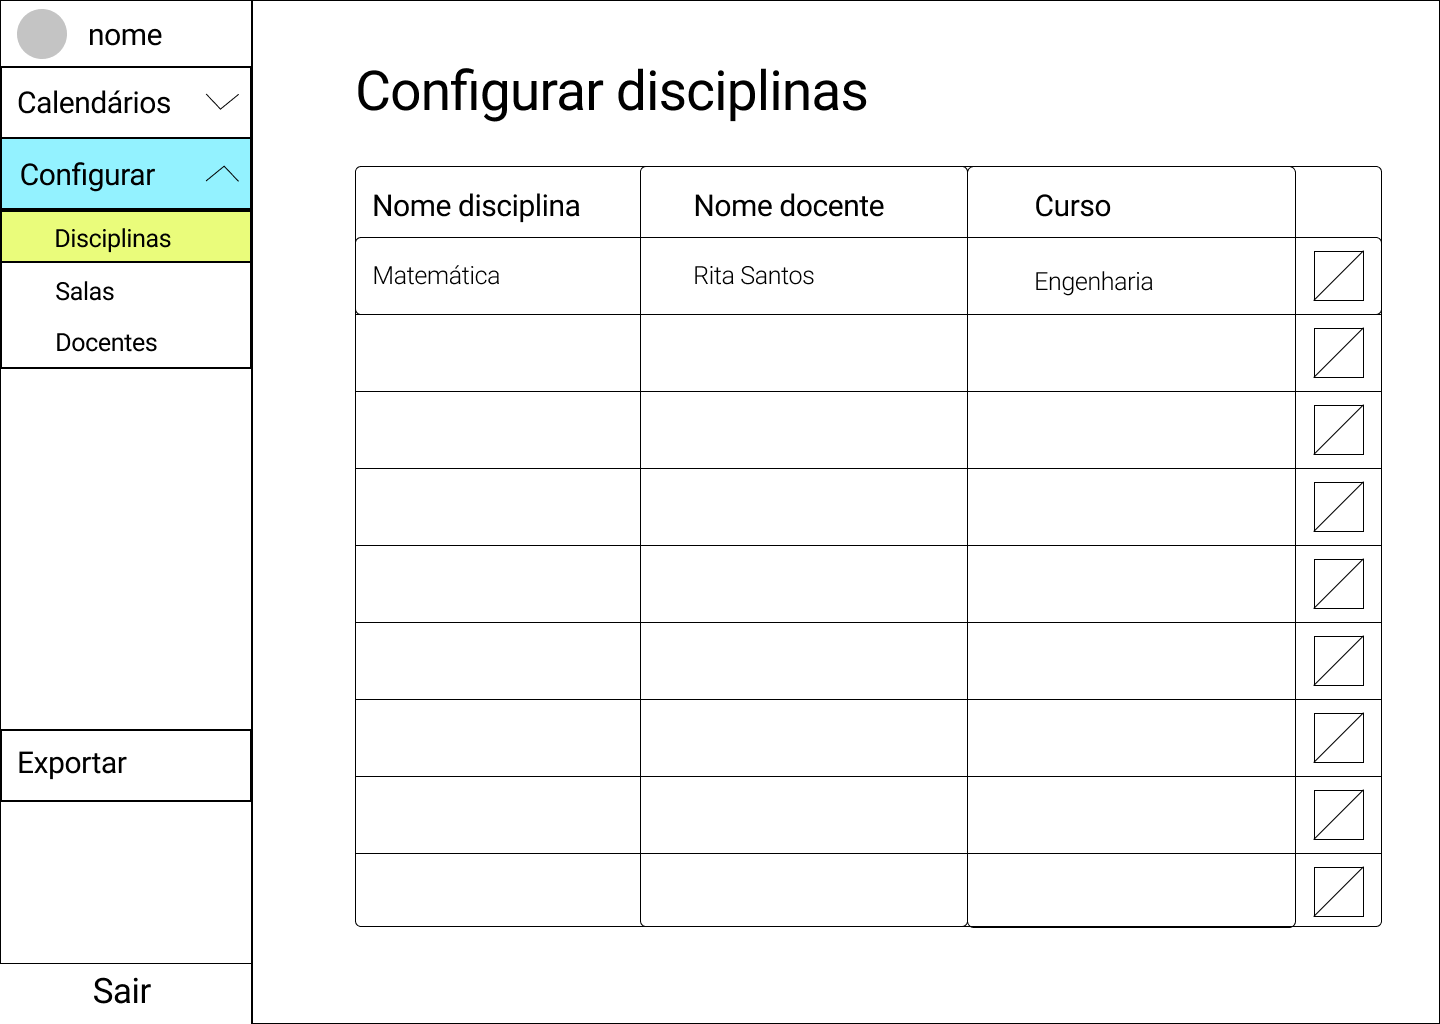
\includegraphics[width=0.8\textwidth,height=0.8\textheight,keepaspectratio]{image/prototipowireframes/configurardisciplinas}
		\caption{Interface para configurar disciplinas}
		\label{interfaceconfdisciplinas}
	\end{figure}

	
		\begin{figure}[H] 
		\centering 
		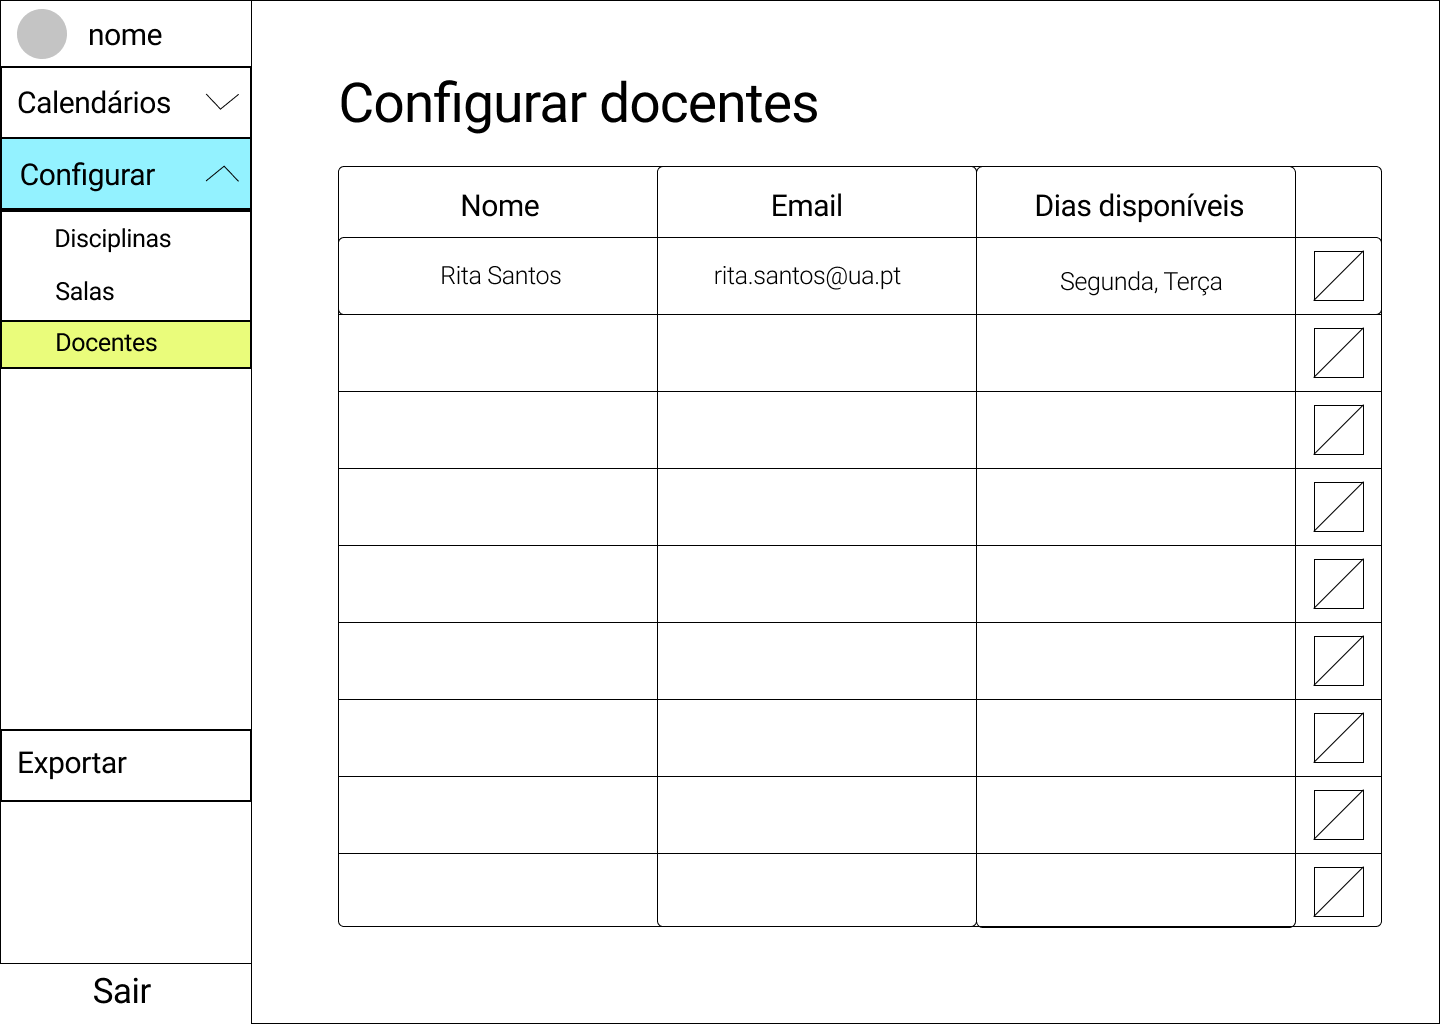
\includegraphics[width=0.8\textwidth,height=0.8\textheight,keepaspectratio]{image/prototipowireframes/configurardocentes}
		\caption{Interface para configurar docentes}
		\label{interfaceconfdocentes}
	\end{figure}
	
	\begin{figure}[H] 
		\centering 
		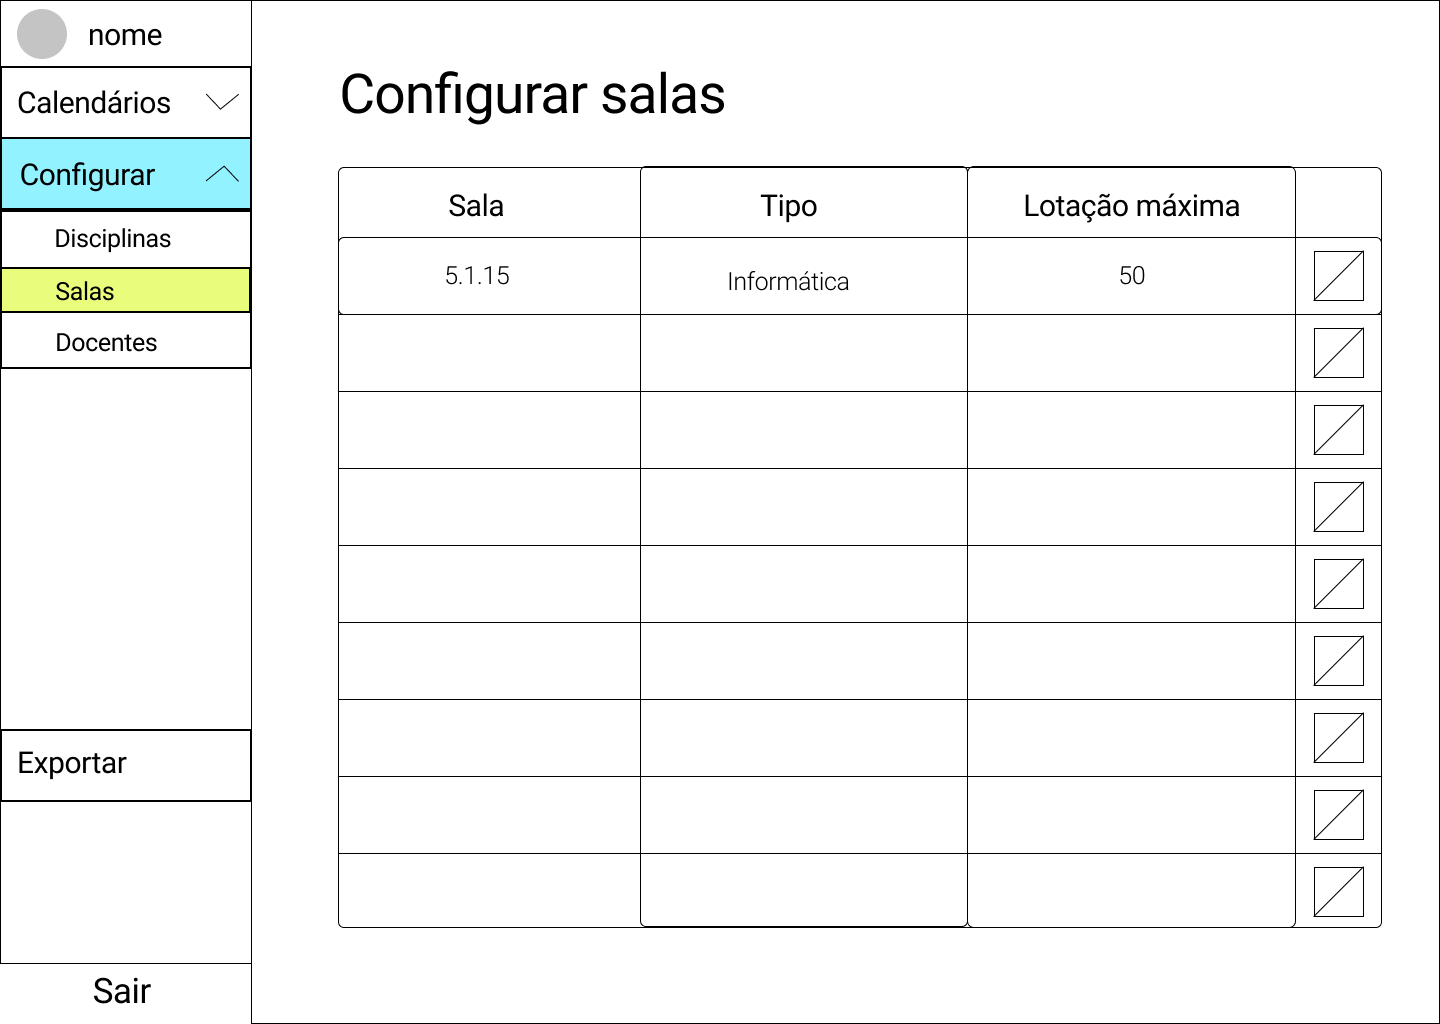
\includegraphics[width=0.8\textwidth,height=0.8\textheight,keepaspectratio]{image/prototipowireframes/configurarsalas}
		\caption{Interface para configurar salas}
		\label{interfaceconfsalas}
	\end{figure}

\def\arraystretch{1.5}
\begin{table}[H]
	\caption{Caso de utilização - Exportação do calendário em formato pdf}
	\begin{center}	
		\begin{tabularx}{\textwidth}{|l|X|}
			\hline
			\textbf{Nome }	& \textbf{Exportação do calendário em formato pdf} \\
			\hline
			Atores: & Utilizador \\
			\hline
			Prioridade: & Alta \\
			\hline
			Requisitos funcionais:& RF.1, RF.2, RF.25, RF.26 \\
			\hline
			Finalidade: & Aceder às funcionalidades da aplicação\\
			\hline
			Sumário: & Após a criação dos calendários o utilizador pode exportar em pdf um calendário ou um conjunto de calendários dos vários cursos. \\
			\hline
			Pré-condições: & Estar conectado à rede da Universidade de Aveiro e ter criado calendários (ver caso de utilização na tabela \ref{usecasecriarcalendario}).\\
			\hline
			Descrição da interação: &  O utilizador seleciona o botão ``Exportar" no menu do lado esquerdo (ver figura \ref{interfaceexportarpdf}) em que aparecerá todos os calendários de cada ano letivo. Terá de selecionar um ano letivo e depois a época e curso. No fim todos os calendáros selecionados serão exportados consoante a época. \\
			\hline
			Cenário alternativo 1:&\textbf{O utilizador seleciona um calendário vazio:} Aparecerá um aviso a indicar que não existe exames marcados no calendário selecionado. No entanto se o utilizador quiser continuar o calendário será exportado.\\
			\hline
			
		\end{tabularx}
	\end{center}
\end{table}

	\begin{figure}[H] 
	\centering 
	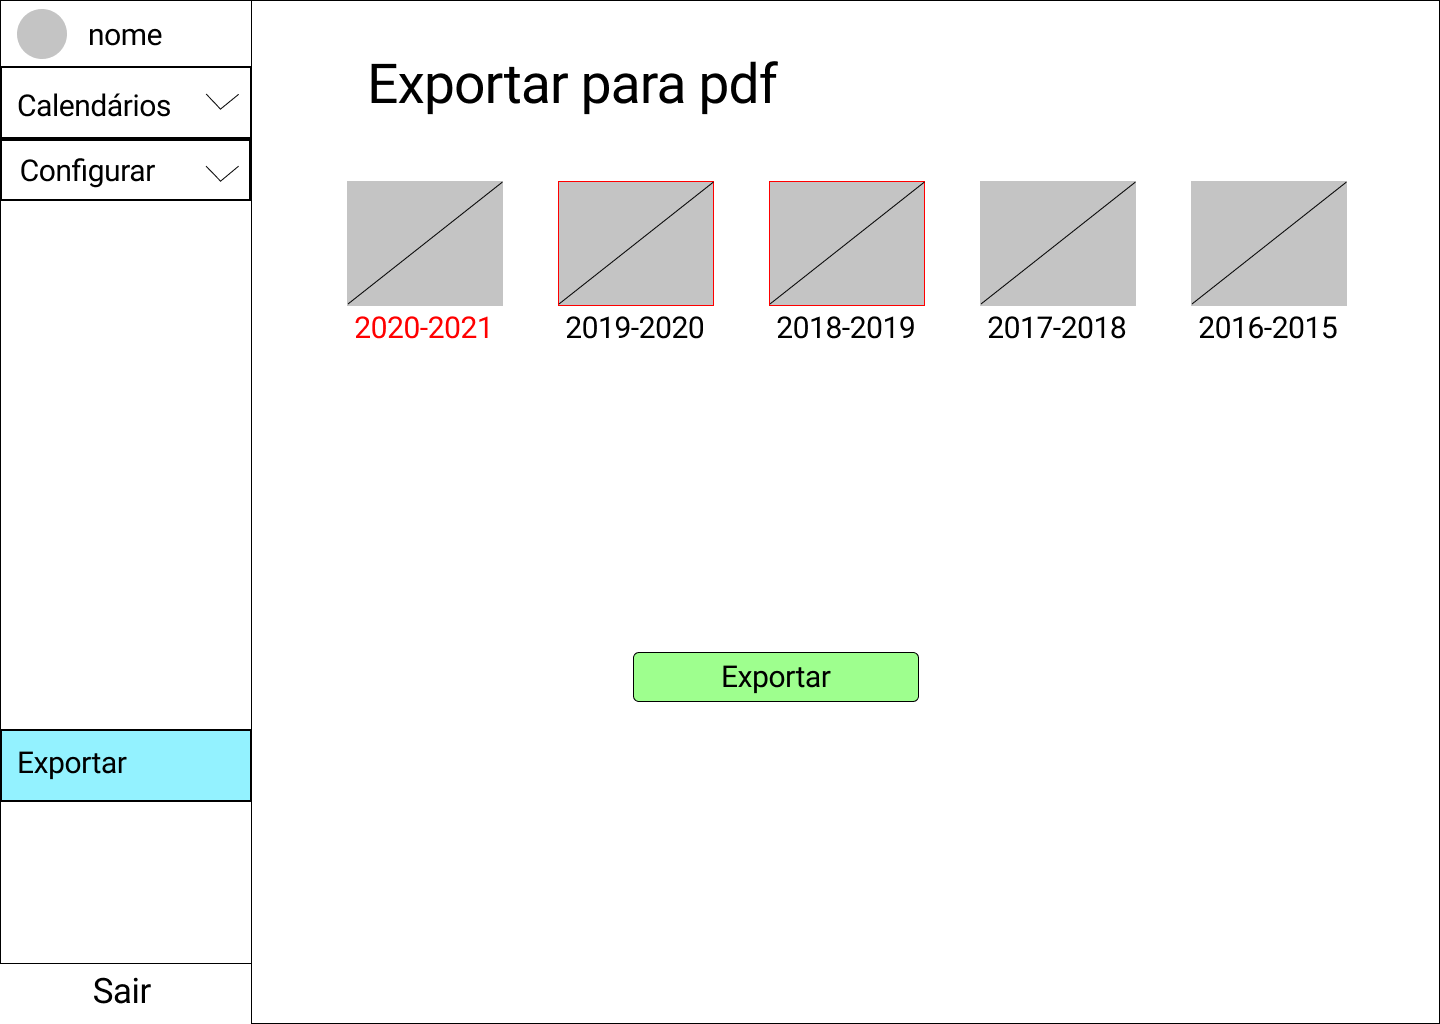
\includegraphics[width=0.8\textwidth,height=0.8\textheight,keepaspectratio]{image/prototipowireframes/exportarpdf}
	\caption{Interface para exportar, em formato pdf, os calendários}
	\label{interfaceexportarpdf}
\end{figure}

\def\arraystretch{1.5}
	\begin{table}[H]
	\caption{Caso de utilização - vizualização do histórico de calendários}
	\begin{center}	
		\begin{tabularx}{\textwidth}{|l|X|}
			\hline
			\textbf{Nome }	& \textbf{Vizualização do histórico de calendários} \\
			\hline
			Atores: & Utilizador \\
			\hline
			Prioridade: & Alta \\
			\hline
			Requisitos funcionais:&  RF.4, RF.26, RF.27, RF.30, RF.31\\
			\hline
			Finalidade: & Visualizar o histórico de calendários\\
			\hline
			Sumário: & O utilizador pode visualizar todos os calendários que já criou em anos anteriores (ver caso de utilização na tabela \ref{usecasecriarcalendario}) ou do mesmo ano letivo que o ano corrente mas no semestre passado. \\
			\hline
			Pré-condições: & Ter iniciado sessão e ter criado calendários\\
			\hline
			Descrição da interação: &  O utilizador pode vizualizar todos os calendários filtrando-os por curso, ano do curso, ano letivo, nome da época e semestre (ver figura \ref{interfacehistorico}). Pode ver os exames marcados, o(s) seus vigilante(s) e a(s) sala(s) associada(s), para além da data de início e fim da época selecionada.\\
			\hline
			Cenário alternativo 1:& \textbf{Quer alterar o horário da marcação dos exames:} Aparecerá um aviso que informa que não pode alterar exames mais antigos que o ano letivo e semestre atual.\\
			\hline
			Cenário alternativo 2:& \textbf{Quer visualizar todos os calendário dos 3 anos de um curso específico:} Seleciona o curso, ano letivo, época, semestre e na opção ``ano'' do curso escolhe ``todo'' e aparecerá todos os anos na mesma página.\\
			\hline
		\end{tabularx}
	\end{center}
\end{table}

	\begin{figure}[H] 
	\centering 
	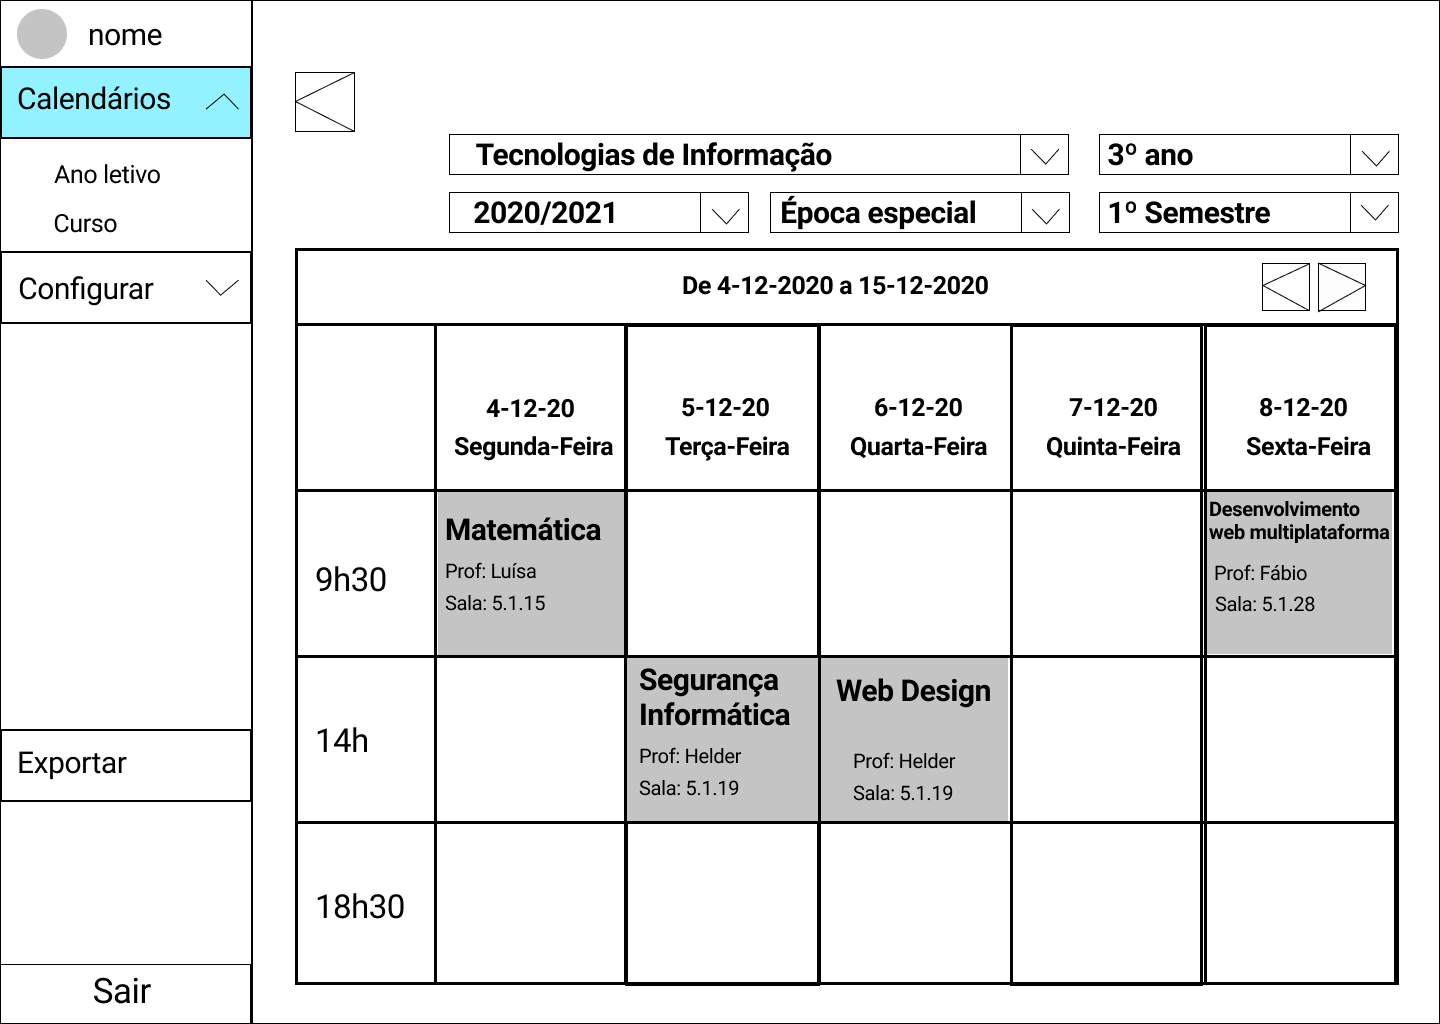
\includegraphics[width=0.8\textwidth,height=0.8\textheight,keepaspectratio]{image/prototipowireframes/calendariohistorico}
	\caption{Interface para visualizar o histórico dos calendários}
	\label{interfacehistorico}
\end{figure}

	
	\chapter{Prototipagem}
	
	\section{Protótipo de baixa fidelidade não funcional}
	\label{prototipobaixafidelidade}
	
	Antes de uma primeira implementação em web escolheu-se um template para se basear o protótipo de baixa fidelidade não funcional. O template (ver figura \ref{template}) pode ser encontra-do a partir do link \href{https://adminlte.io/themes/v3/pages/calendar.html}{https://adminlte.io/themes/v3/pages/calendar.html} e tem a licença MIT. Com isto protipou-se todos os casos de utilização da primeira e da segunda fase.
	
	\begin{figure}[H] 
		\centering 
		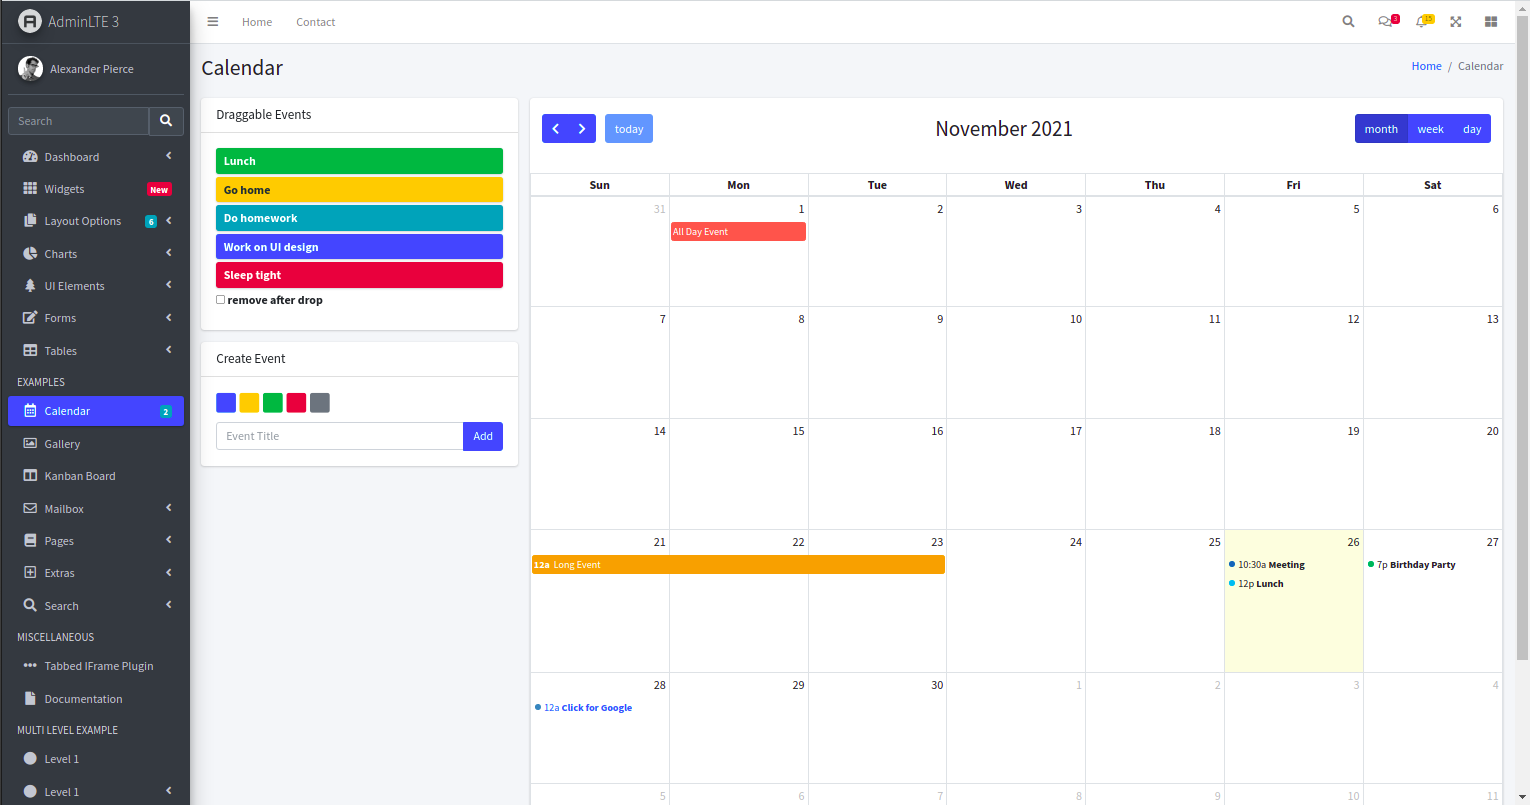
\includegraphics[width=0.8\textwidth,height=0.8\textheight,keepaspectratio]{image/template}
		\caption{Template escolhido para se basear a aplicação}
		\label{template}
	\end{figure}
	
	\subsection{Wireframes}
	
	Nos wireframes - protótipo de baixa fidelidade não funcional - as funcionalidades foram dividas em 3 secções no menu: calendários, configurar e exportar. Dentro do menu na opção ``calendários'' o utilizador pode criar novos calendários ou visualizar o histórico de calendários mais antigos podendo filtrar por ano letivo ou curso, como se pode ver na figura \ref{menucalendario}. A opção que está selecionada apresenta uma cor diferente do restante menu. Para além disso a distinção de calendários antigos e recentes é feita por duas cores: a verde são os calendários ``fechados'' e a vermelho são os que podem ser editados. 
	
	\begin{figure}[H] 
		\centering 
		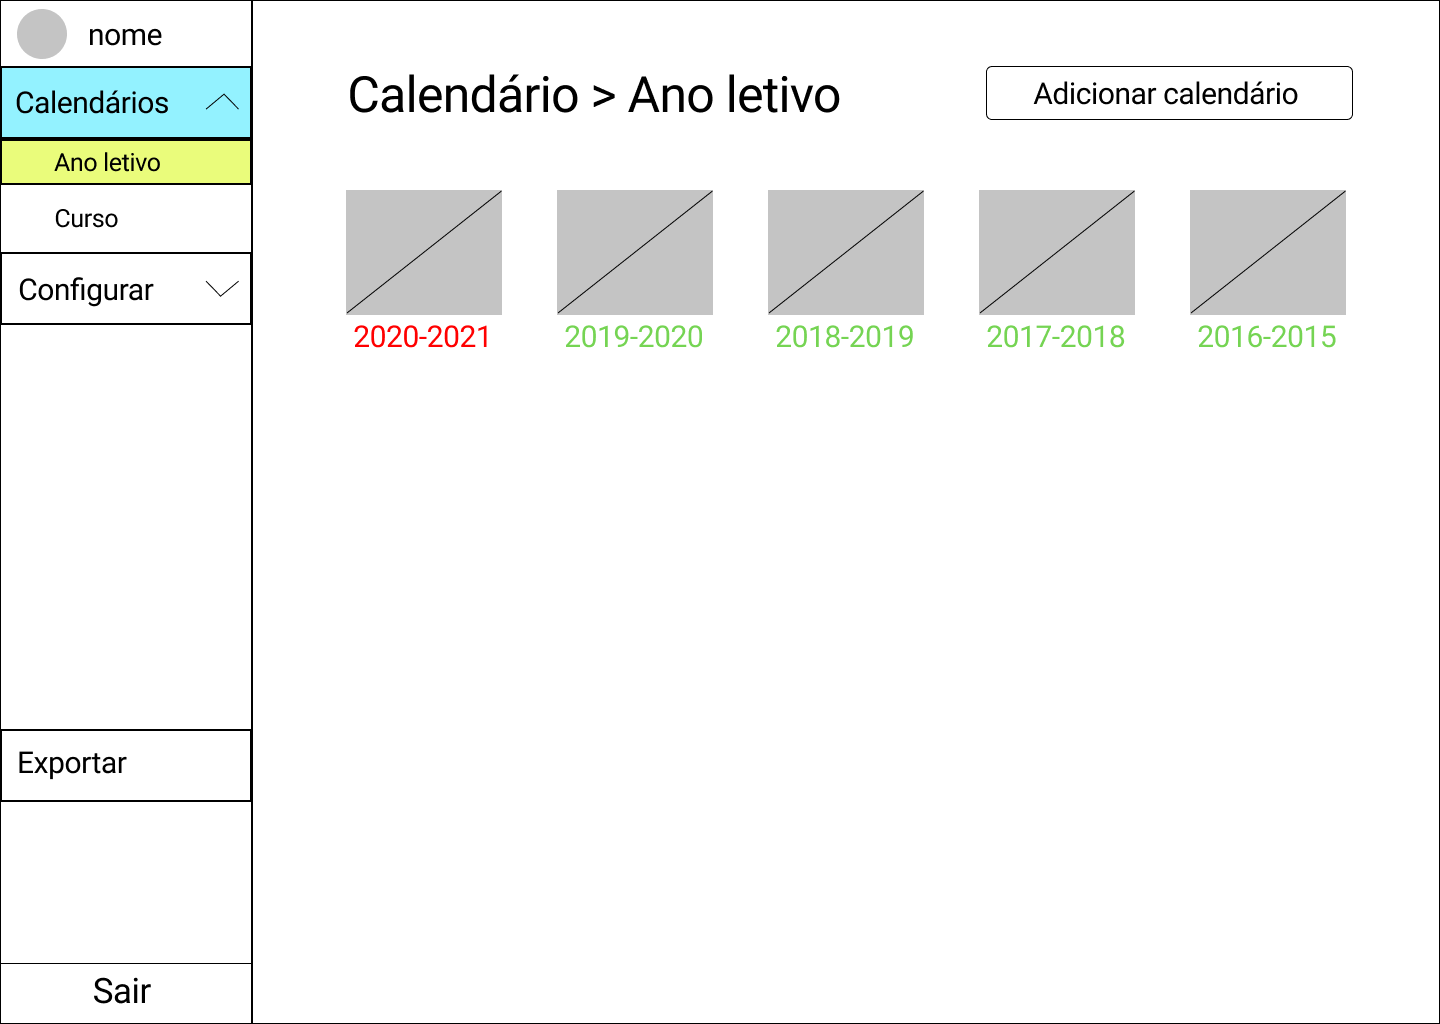
\includegraphics[width=0.8\textwidth,height=0.8\textheight,keepaspectratio]{image/prototipowireframes/pesquisacalendarioanoletivo}
		\caption{Pesquisar calendários a partir do ano letivo}
		\label{menucalendario}
	\end{figure}
	
	Dentro da secção ``configurar'' (ver figura \ref{configurarsalas}) estam todas as informações que o utilizador necessita para a criação dos calendários e a marcação de exames. Estas podem ser importados a partir de um ficheiro .csv ou o próprio pode adicionar na aplicação . 
	
	 
	\begin{figure}[H] 
		\centering 
		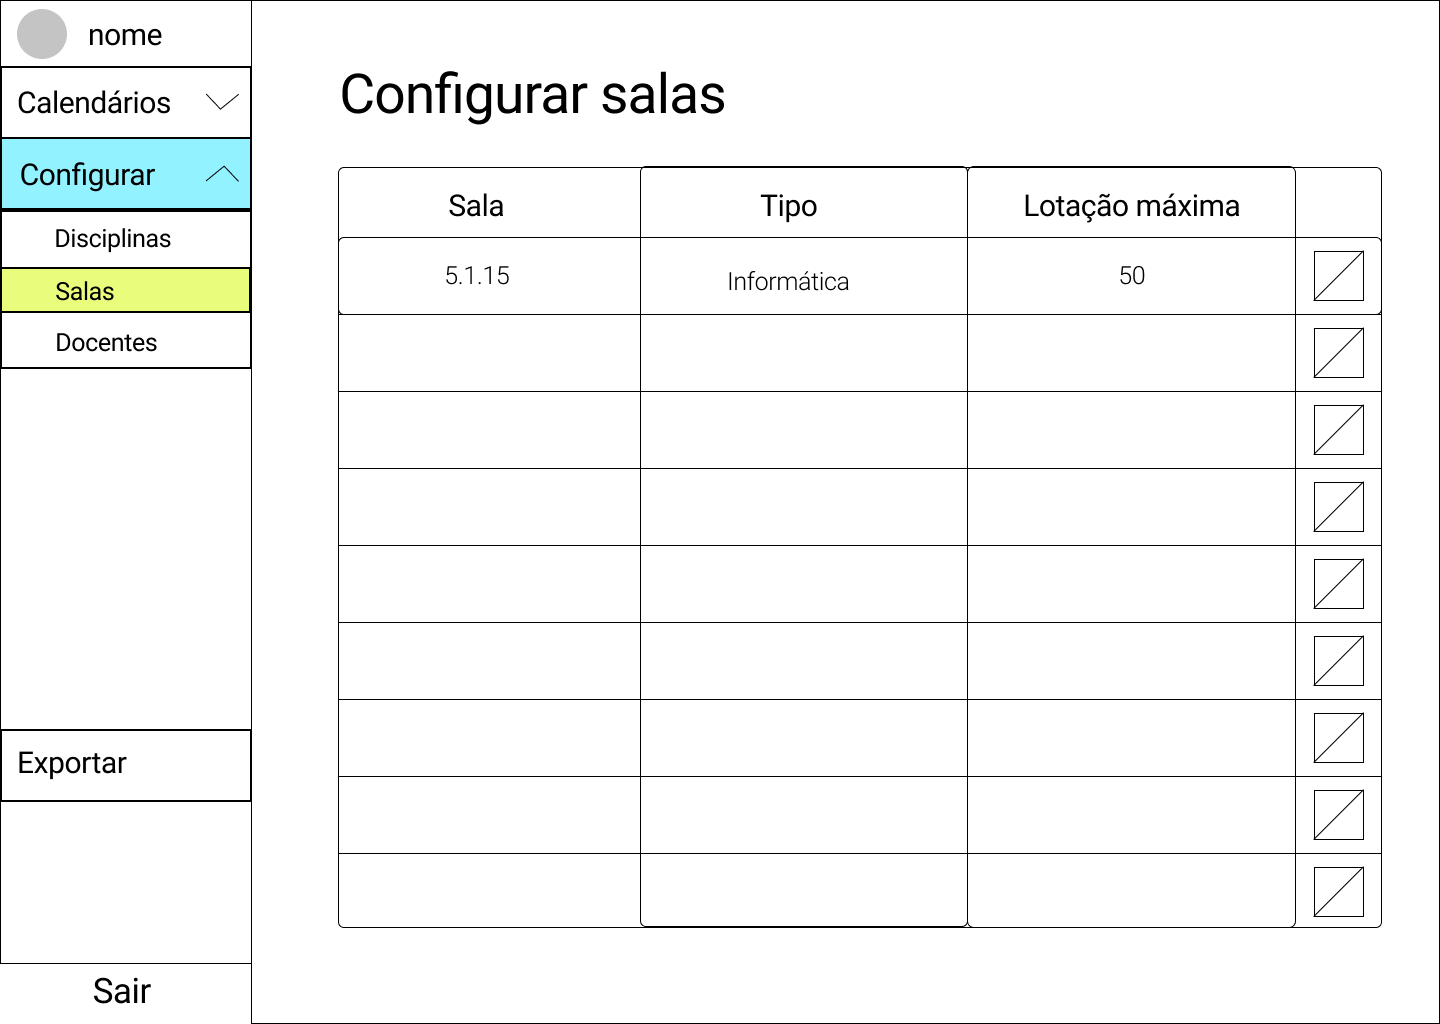
\includegraphics[width=0.8\textwidth,height=0.8\textheight,keepaspectratio]{image/prototipowireframes/configurarsalas}
		\caption{Visualização de informações sobre as salas}
		\label{configurarsalas}
	\end{figure}

Dentro da secção ``exportar"  (figurar \ref{exportar}) o utilizador pode exportar para pdf os calendários que selecionar.


	\begin{figure}[H] 
	\centering 
	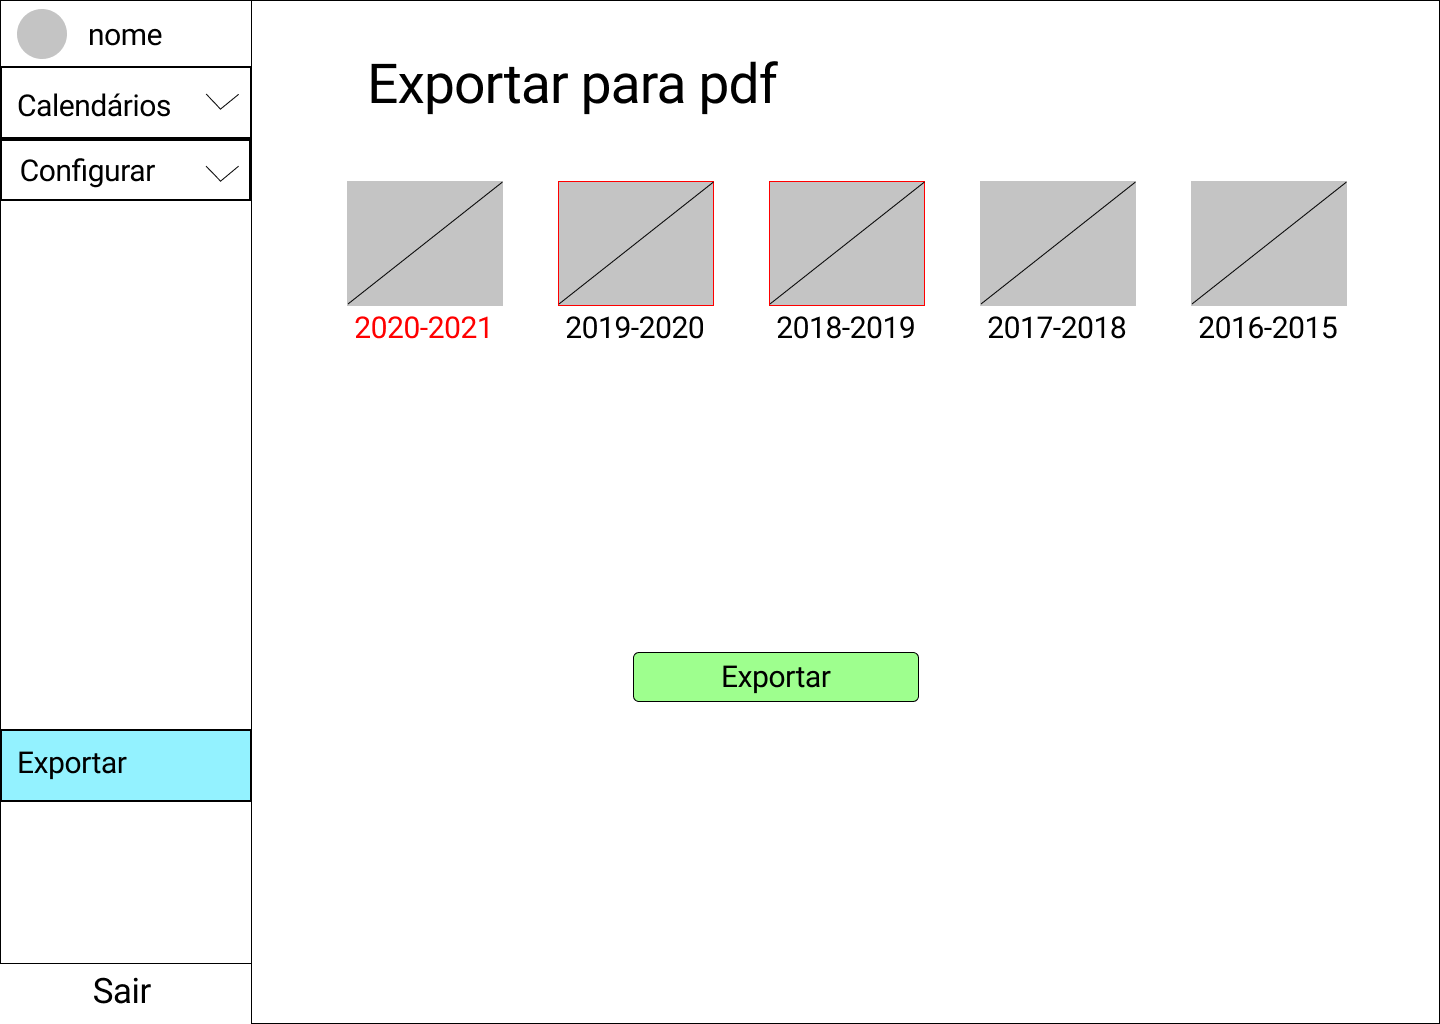
\includegraphics[width=0.8\textwidth,height=0.8\textheight,keepaspectratio]{image/prototipowireframes/exportarpdf}
	\caption{Visualização de informações sobre as salas}
	\label{exportar}
\end{figure}

	
	\subsection{Diagrama de user flow}

	Com o desenvolvimento dos wireframes criou-se o diagrama de user flow que é útil para entender quais são os passos que o utilizador terá de realizar para concluir uma tarefa. Este diagrama foi desenvolvido consoante os wireframes e a descrição dos casos de utilização.

	\begin{landscape}
		\pagestyle{empty}
		\begin{figure}[H] 
			\centering 							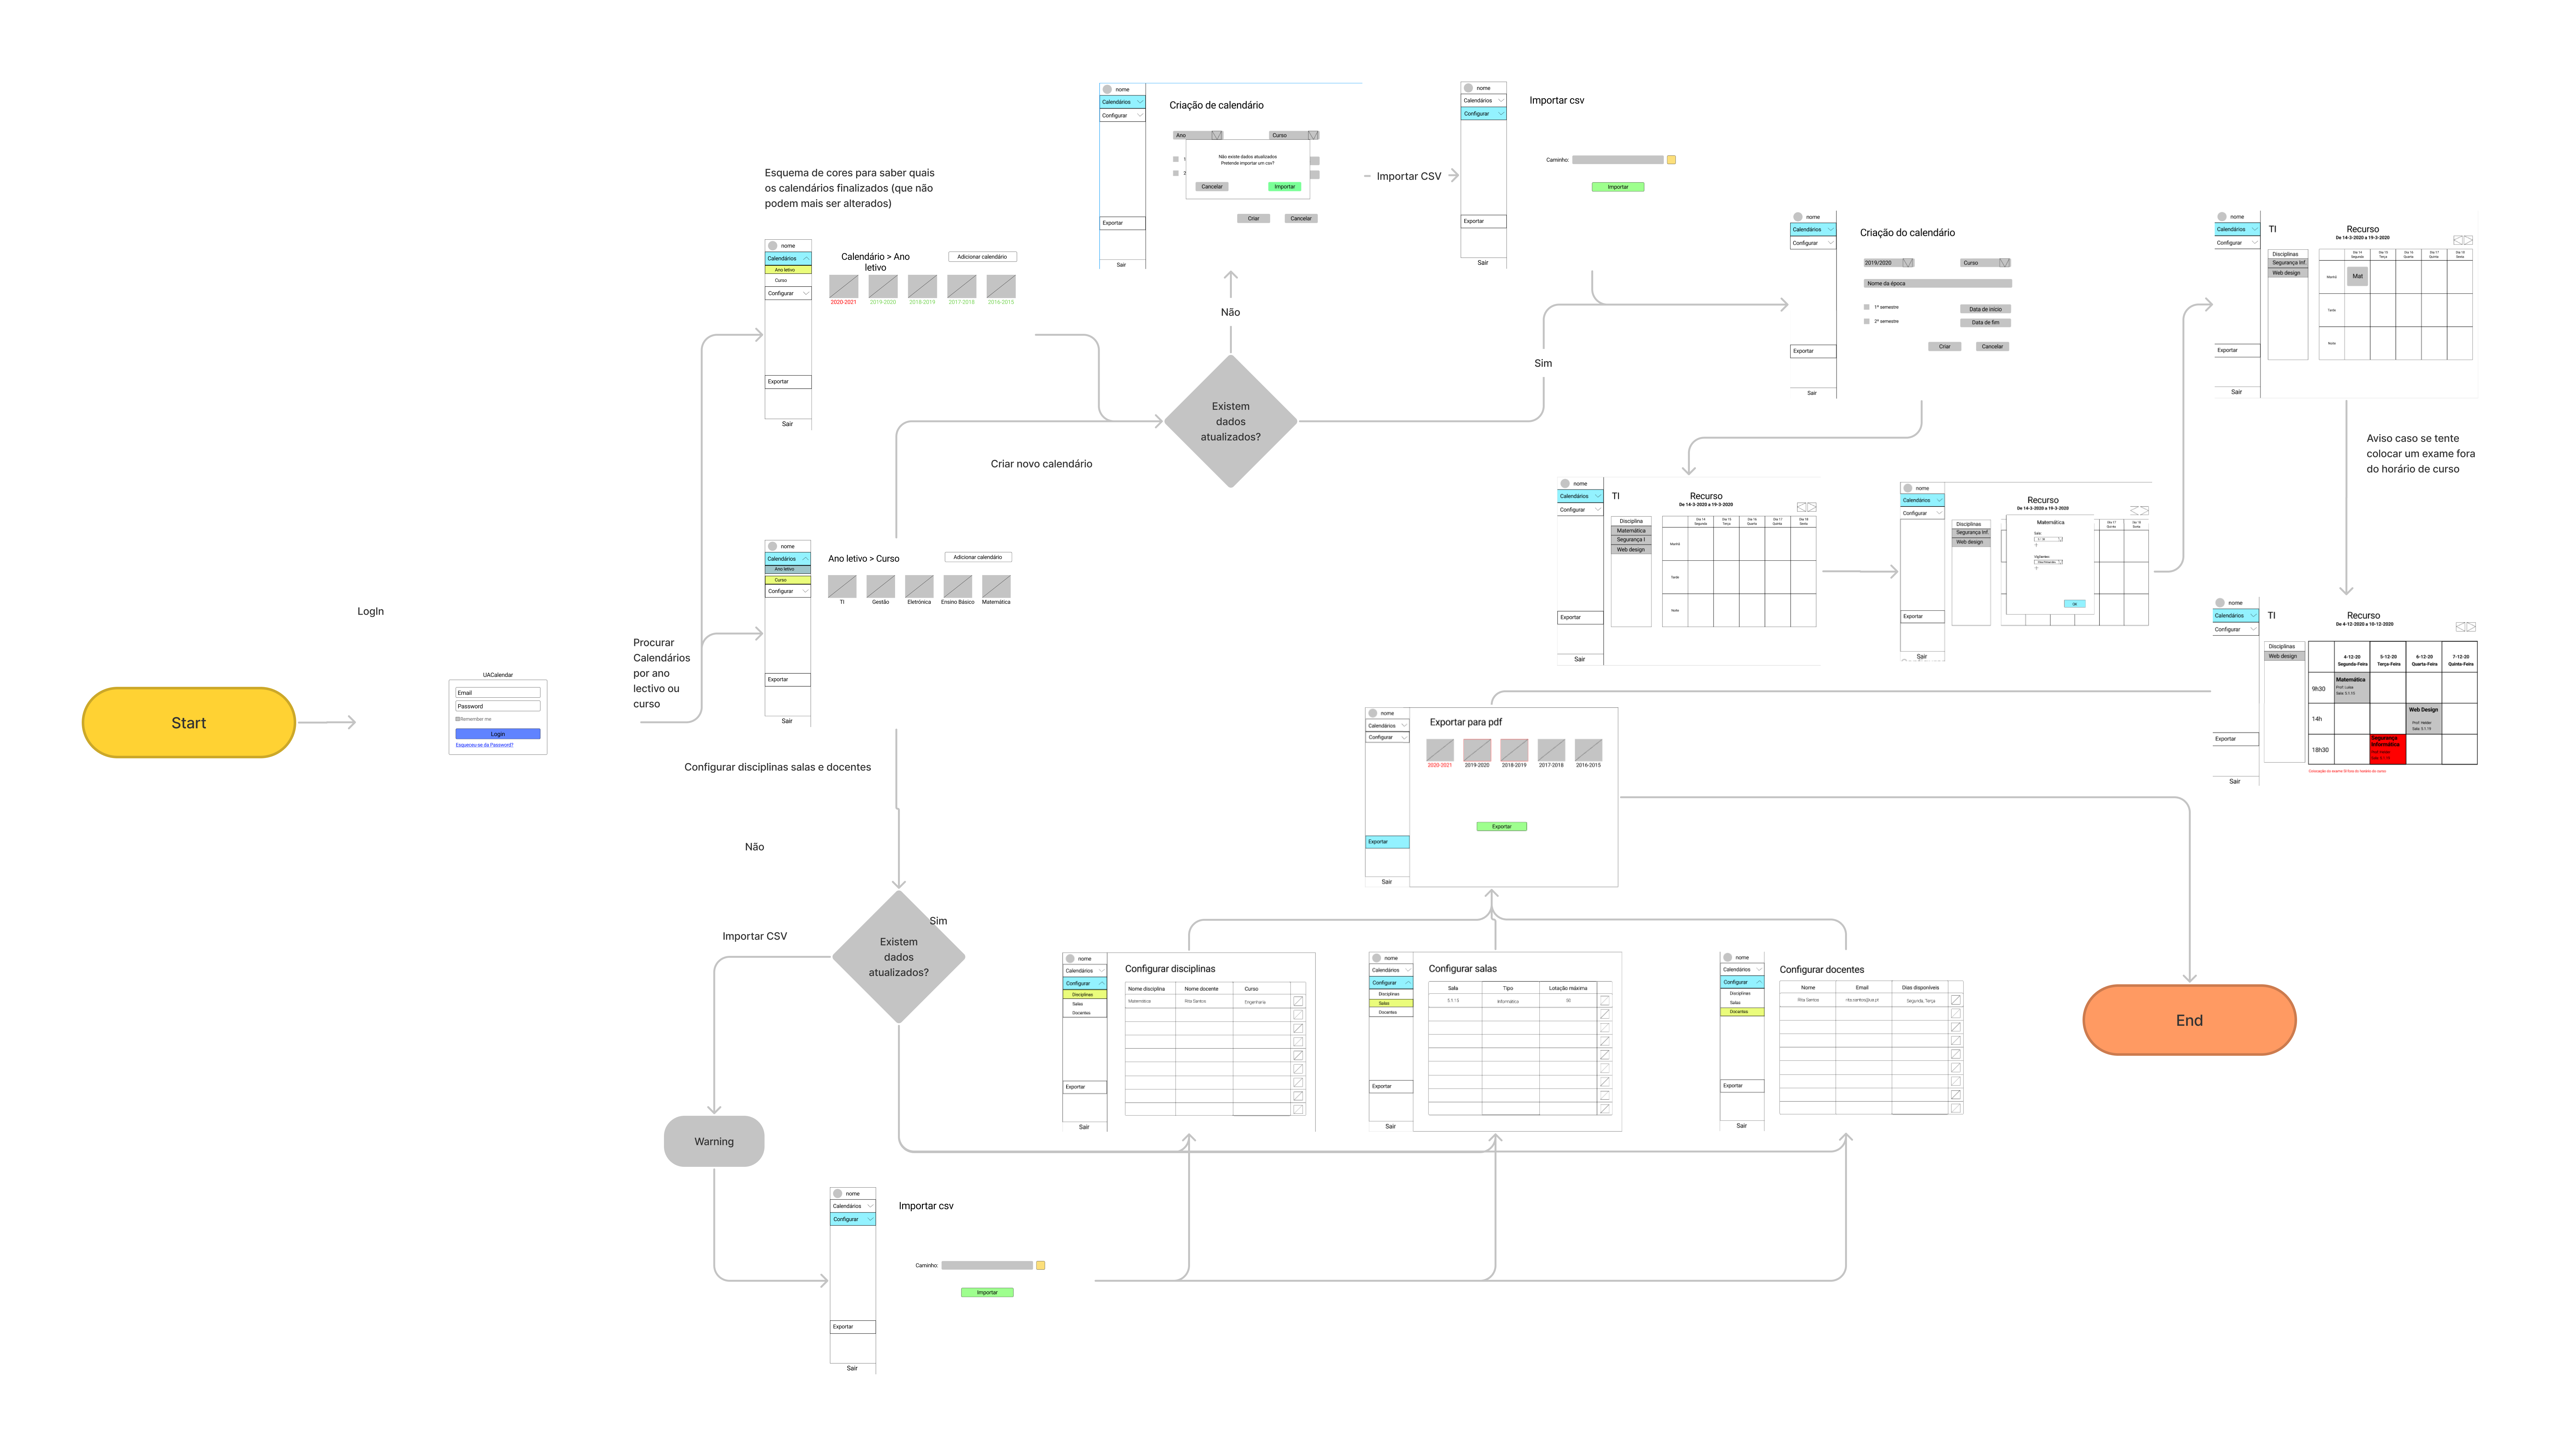
\includegraphics[width=1.5\textwidth,height=1.5\textheight,keepaspectratio]{image/diagramauserflow}
			\caption{Diagrama de user flow}
		\end{figure}
	\end{landscape}

	\subsection{Testes}
	\label{primeiroTeste}
		Após a interface da aplicação estar idealizada e terem sido concluídos os protótipos de baixa fidelidade, foi programada uma sessão de avaliação com a participação de dois utilizadores participantes, o Sr. Paulo e a professora Magda Monteiro, de modo a podermos obter feedback e avaliar se a interface em questão consegue satisfazer os requisitos que são propostos. Para que esta sessão de avaliação podesse ocorrer, além dos utilizadores participantes era necessária a presença de um moderador e de pelo menos dois observadores. Foram ainda preparados três documentos de apoio à sessão: um guião de apoio ao moderador, um guião para os utilizadores participantes e uma grelha de observação para os elementos observadores - que podem se observar nos anexos A, B e C. A estrutura de ambos os guiões é semelhante, apresentando uma capa, uma pequena introdução que explica os objetivos da sessão e as tarefas a desempenhar, apenas difere no guião do moderador, que também tem presente o que é necessário para preparar a sessão e as ``regras" pela qual este se deverá reger durante a realização da mesma. Para preparar a sessão é necessária a existência de um computador, um browser instalado e acesso à internet de modo a poder aceder ao website onde estão alojados os protótipos de baixa fidelidade (\href{https://www.figma.com/file/nhb5nnIrt3fdDoQhYpsN80/Calendario?node-id=9\%3A154}{\textbf{wireframes}}).

Foram selecionadas nove tarefas com base nos protótipos desenhados para o utilizador participante desempenhar:

\begin{itemize}
	\item Verificar o calendário final de Ti do ano letivo 2019/2020;
	\item Importar ficheiro .csv;
	\item Verificar individualmente quantas disciplinas, salas e docentes existem;
	\item Pesquisar por "Ti" na barra de pesquisa e abrir o calendário "Ti - 1º Ano - 1º Semestre";
	\item Criar um novo calendário para o curso de Ti;
	\item Mover matemática para o período da manhã do dia 14;
	\item Colocar "Segurança Inf." num período da noite;
	\item Exportar para um .pdf;
	\item Fazer Log Out.
\end{itemize}


Durante a sessão de avaliação o papel de moderador foi desempenhado pela Sofia Rocha e o papel de observador foi desempenhado pelo Bruno Lopes, Gonçalo Tavares e o Leandro Silva cujas grelhas de observação individuais ao serem unidas num único documento por utilizador participante resultaram nos ficheiros que se encontram presentes no anexo C.

	

	\subsubsection{Análise de resultados}
Concluída a sessão de avaliação e a posterior junção das grelhas dos observadores, o grupo passou ao momento da análise dos resultados em conjunto com a professora Rita durante a reunião semanal do projeto. Desta análise resultou um conjunto de alterações que foram aplicadas aos protótipos de baixa fidelidade, sendo estas as seguintes alterações:

\begin{itemize}
	\item Abrir diretamente a página da configuração das disciplinas ao selecionar o menu configurar;
	\item Adicionar um sistema de calendários editáveis e fechados distinguíveis através de uma label aberto/fechado e/ou um sistema de cores;
	\item Alterar a localização do botão importar;
	\item Destacar o botão novo e alterar a sua posição na página para o canto superior direito;
	\item Pedir ao utilizador para importar um ficheiro .csv na primeira vez que o mesmo for criar um novo ano letivo, caso ainda não exista informação referente a esse ano letivo na base de dados;
	\item Remover o menu de registo de contas;
	\item Remover o submenu ``época" do menu ``Calendários";		
	\item Separar o botão exportar dos restantes elementos do menu e acrescentar um segundo botão exportar no canto superior direito junto do botão novo.

\end{itemize}

	\section{Protótipo de alta fidelidade não funcional}
	
	Na segunda fase do projeto criou-se o protótipo de alta fidelidade não funcional utilizando laravel mas sem nenhuma conexão a uma base de dados. Inicialmente houve uma adaptação do template - mencionado na secção \ref{prototipobaixafidelidade} - para o laravel. Este protótipo pode ser visualizado através do \href{http://estga-dev.clients.ua.pt/~ptdw-2021-gr4}{$\underline{link}$}  disponibilizado pela ESTGA dentro da rede da Universidade de Aveiro ou através da sua VPN.
	
	\subsection{Desenvolvimento do protótipo}
<<<<<<< Updated upstream
=======
	
	Durante a transição dos wireframes para o protótipo de alta fidelidade não funcional fez-se as várias alterações mecionadas nos testes - secção \ref{primeiroTeste}. No entanto ao longo do desenvolvimento do protótipo ocorreram várias alterações tanto na organização do menu como no aspeto gráfico.
	
	Inicialmente o utilizador terá de iniciar sessão e por isso aparece a página da figura \ref{login}, no entanto como não tem ligação à base de dados o utilizador pode prosseguir para a seguinte página sem inserir dados. 
	
	\begin{figure}[H] 
		\centering 							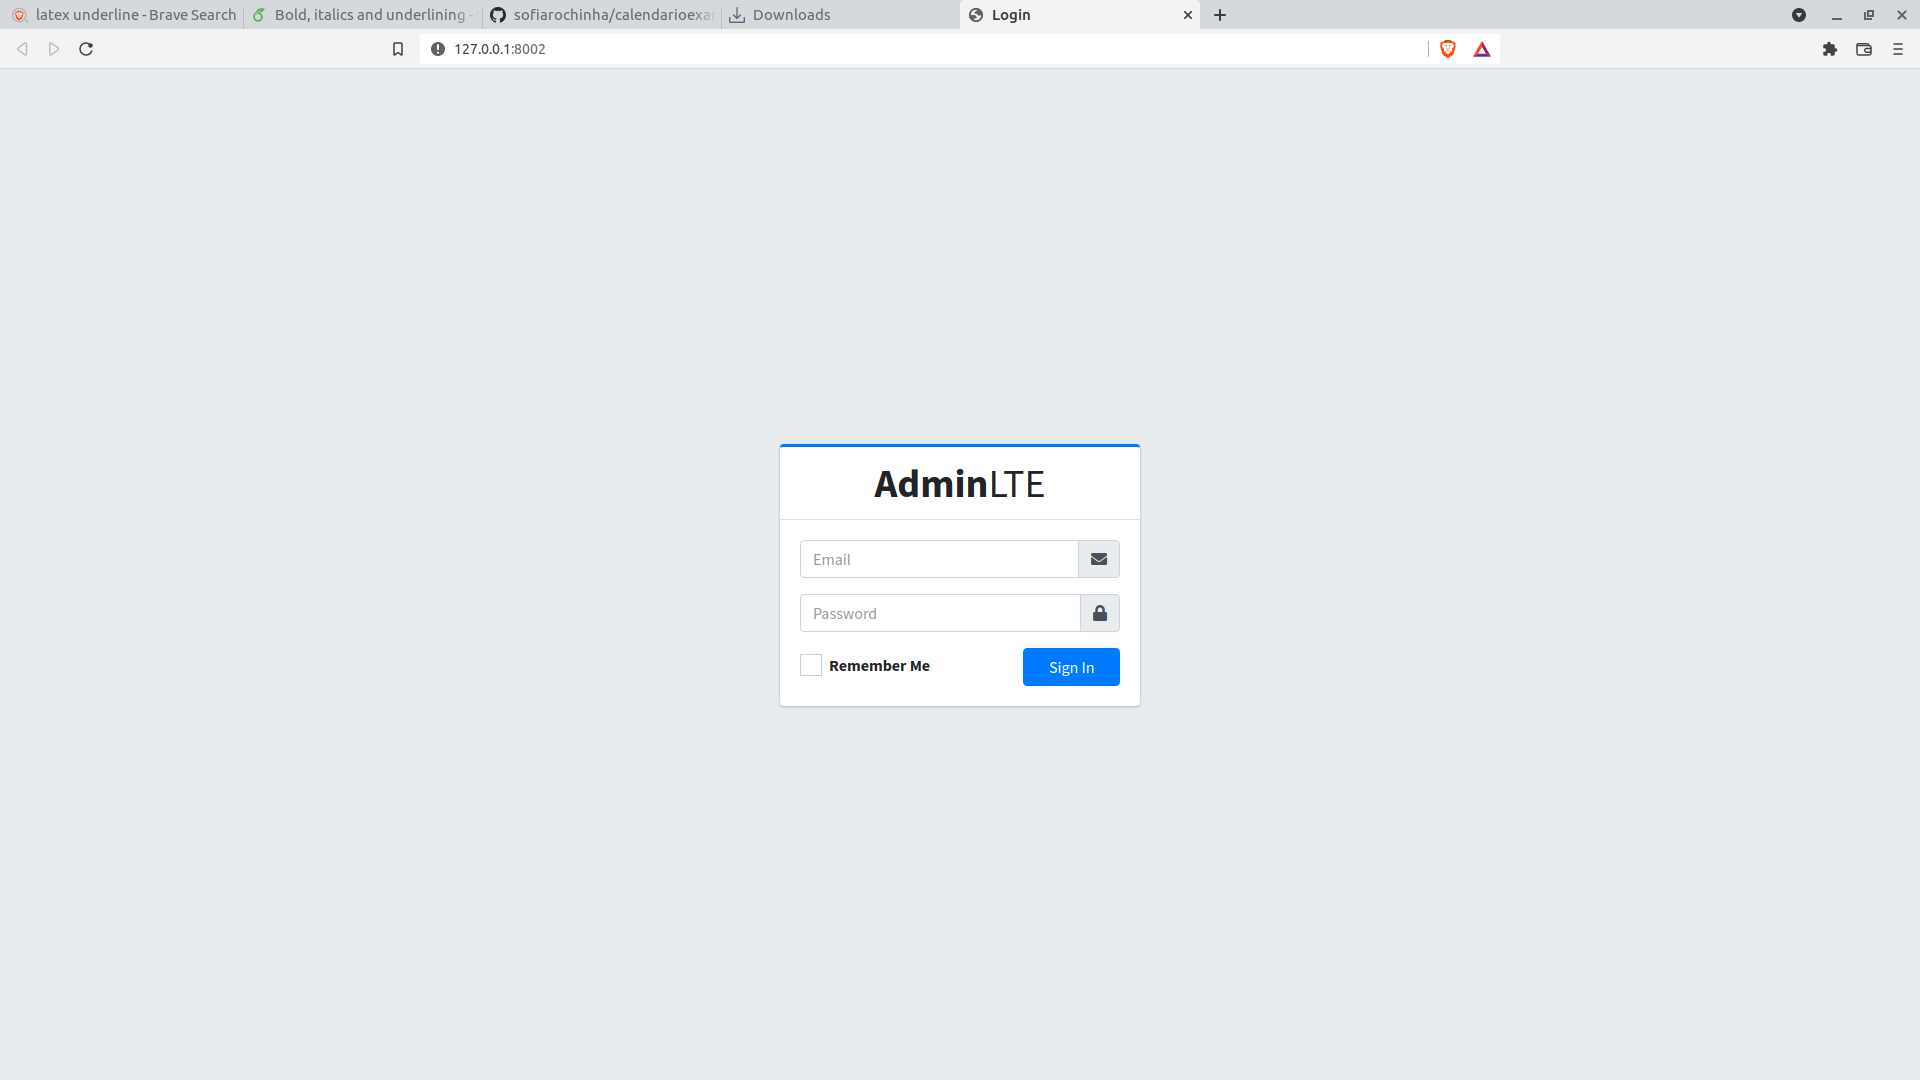
\includegraphics[width=0.8\textwidth,height=0.8\textheight,keepaspectratio]{image/PrototipoAFNF/login}
		\caption{Interface para iniciar sessão}
		\label{login}
	\end{figure}
	
	Assim que entra na aplicação a primeira página que aparece é a de selecionar um curso (ver figura \ref{selecionarCurso}) para visualizar o calendário de exames do mesmo. Nesta página é visível uma reorganização do menu (inspirado pelo ``Outlook Calendar'' e pelo ``Google Calendar") em relação aos wireframes. O menu começa com o ``criar calendário" em que está sempre destacado porque é uma ação importante e que se irá repetir várias vezes. De seguida tem o ``Calendário Atual'' que tem dois opções: ``Visualizar'' - que permite visualizar todos os calendários atuais e marcar os respetivos exames - e ``Configurações'' - que são todas as configurações, das unidades curriculares, docentes, salas e épocas do semestre corrente, que foram importadas do ficheiro .csv. Logo abaixo tem o importar CSV seguido de exportar que são duas ações parecidas. Por fim tem os calendários anteriores que é algo que se espera que o utilizador vá utilizar muito raramente e no final do menu tem a opção de encerrar a sessão.
	
	Para além da alteração do menu foi adiconado em todas as páginas \textit{breadcrumbs} para facilitar o utilizador a retrodecer para a página inicial ou identificar em que página está.  
	
	\begin{figure}[H] 
		\centering 							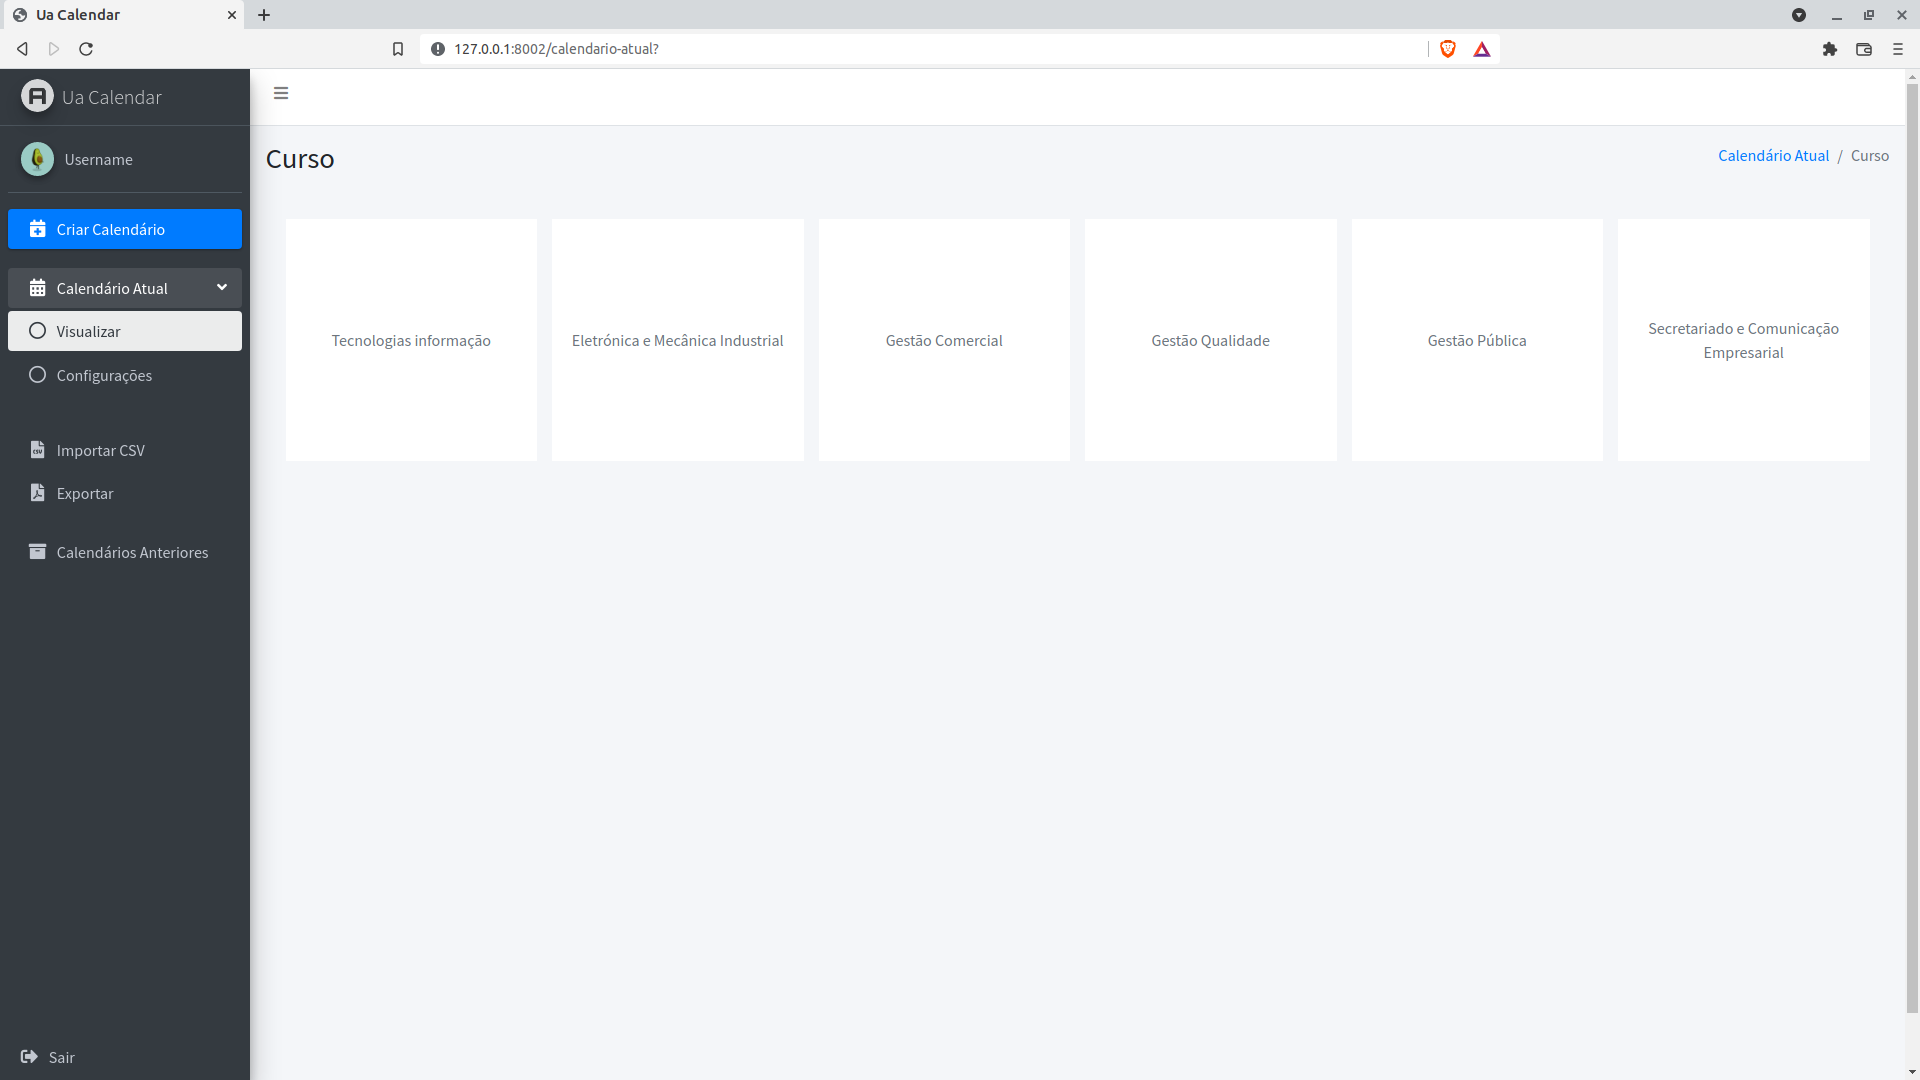
\includegraphics[width=0.8\textwidth,height=0.8\textheight,keepaspectratio]{image/PrototipoAFNF/VisualizarCalendario}
		\caption{Interface onde se seleciona o curso para marcar os exames - primeira página da aplicação}
		\label{selecionarCurso}
	\end{figure}

	Depois de selecionar um curso pode marcar os exames respetivos adicionando através de um popup os vigilantes e as salas. Cada exame está predefinido com uma duração de 4 horas, porque só haverá um exame de manhã, tarde e noite. Para uma melhor acessibilidade foi adicionado várias caixas de seleção para poder mudar de curso, ano do curso e a época de forma mais rápida evitando ter de voltar atrás. 

	\begin{figure}[H] 
		\centering 							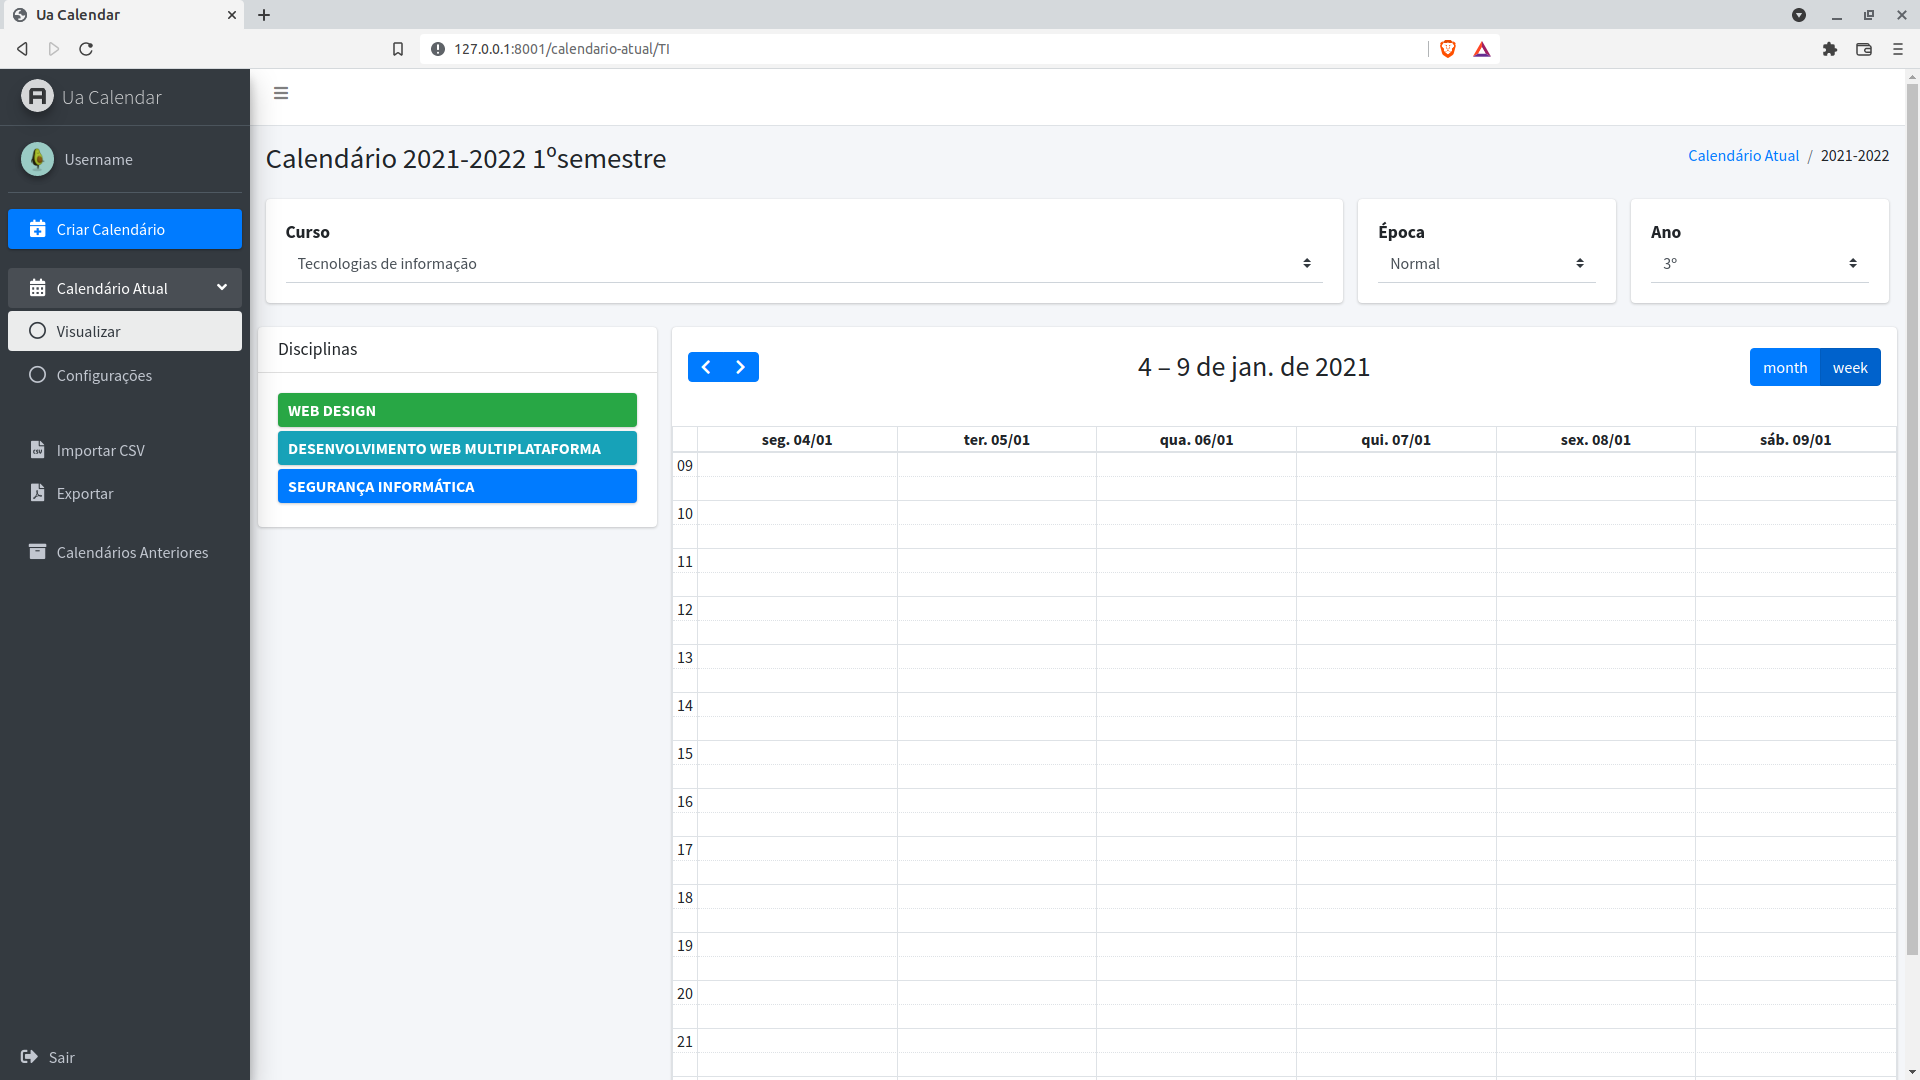
\includegraphics[width=0.8\textwidth,height=0.8\textheight,keepaspectratio]{image/PrototipoAFNF/VerCalendarioAtual}
		\caption{Interface com o calendário atual para marcar os exames}
		\label{marcarExames}
	\end{figure}
	
	No entanto para que os cursos estejam disponíveis o utilizador tem de - a cada semestre - importar um ficheiro .csv, como se pode visualizar na figura \ref{importarCSV}, que contém todos os dados sobre os docentes, salas e cursos. Todas as informações sobre os dados importados encontram-se na página de configurações (ver figura \ref{configuracoes}). 
	
	\begin{figure}[H] 
		\centering 							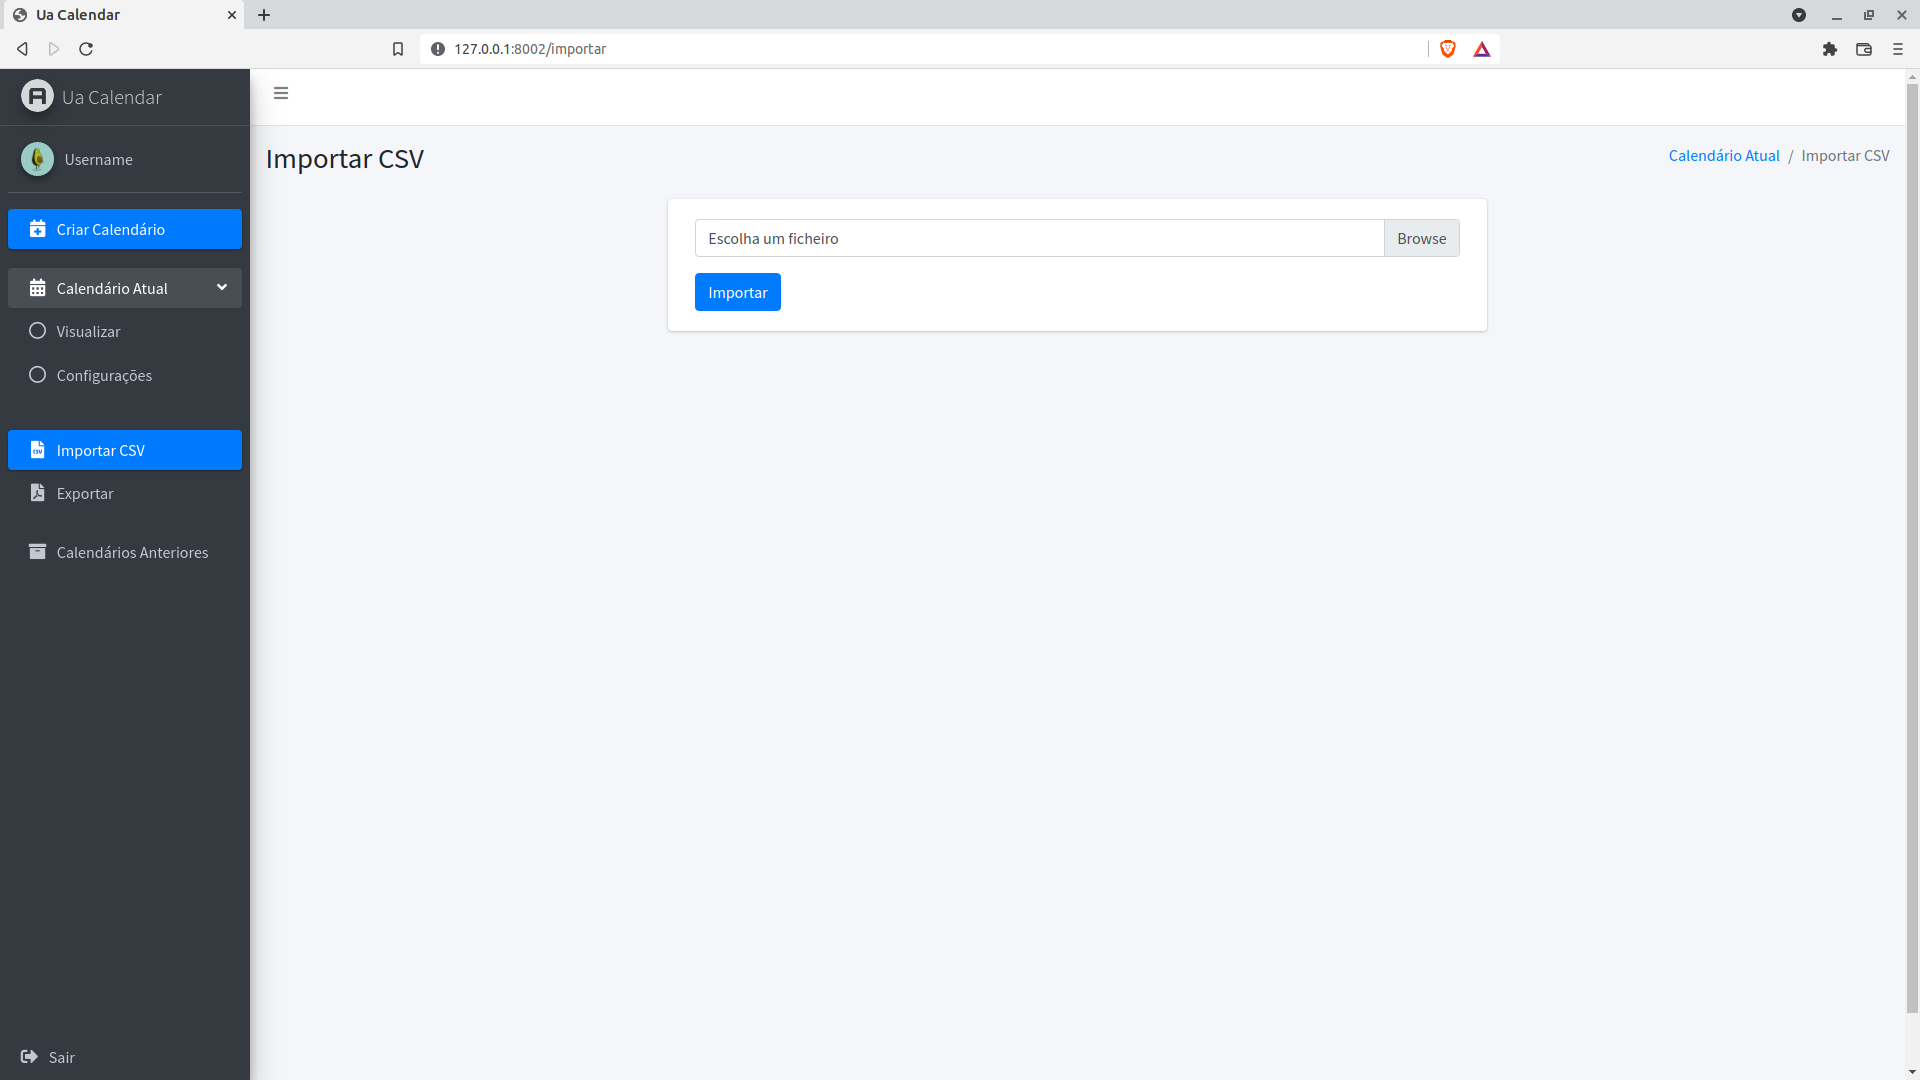
\includegraphics[width=0.8\textwidth,height=0.8\textheight,keepaspectratio]{image/PrototipoAFNF/Importar}
		\caption{Página para importar o ficheiro .csv}
		\label{importarCSV}
	\end{figure}

	Com esta página é possível verificar se todos os dados estam corretos e se tiver algum erro nas informações estas são editáveis. Para além disso se o utilizador pretender pode criar e editar todas as épocas de avaliação na mesma página.  
	
	
	\begin{figure}[H] 
		\centering 							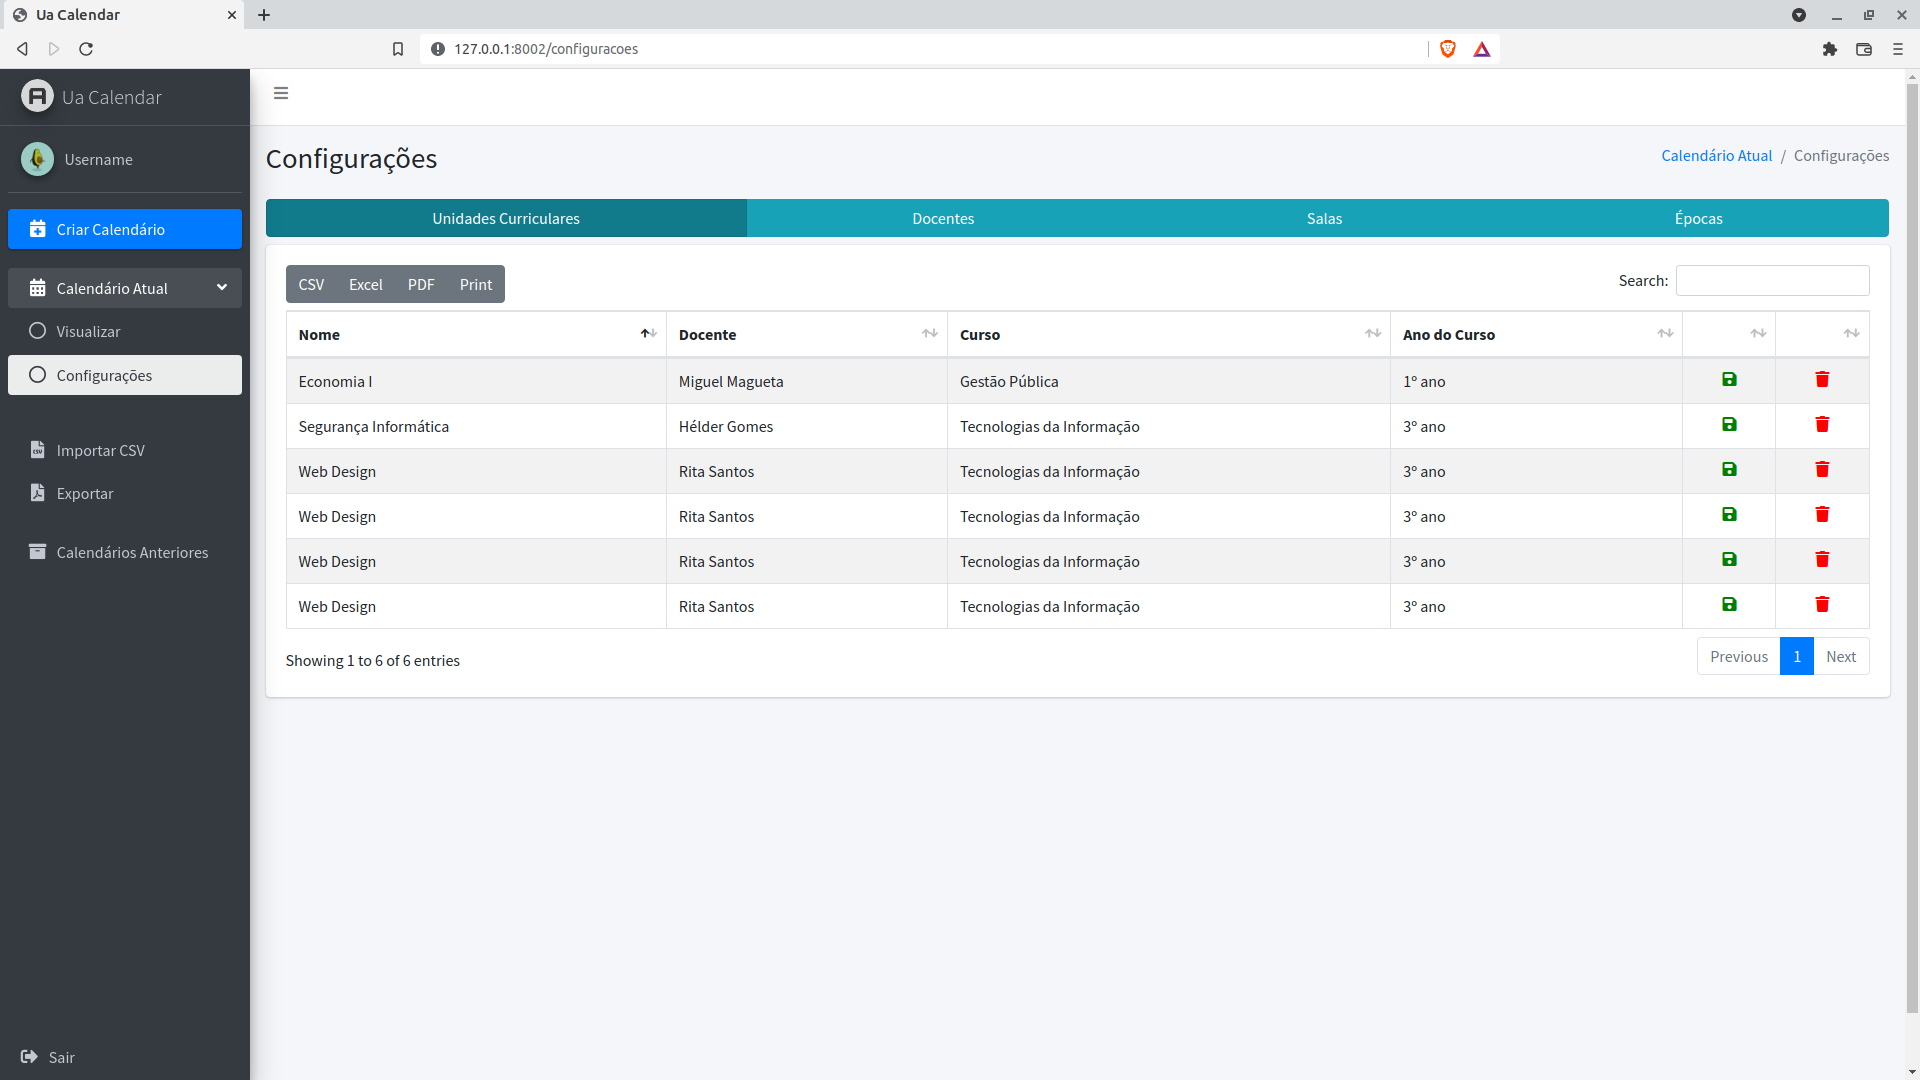
\includegraphics[width=0.8\textwidth,height=0.8\textheight,keepaspectratio]{image/PrototipoAFNF/Configuracoes}
		\caption{Página para visualizar todos os dados importados}
		\label{configuracoes}
	\end{figure}
	
	Após este passo o utilizador pode criar vários calendários de uma só vez, pode adicionar vários cursos, para várias épocas, de vários anos, como mostra a figura \ref{criarCalendario}, ao contrário dos wireframes em que só podia criar um de cada vez. Cada calendário criado pode ser acedido através da opção ``Visualizar'' para marcar os exames pretendidos. 
	
	
	 \begin{figure}[H] 
	 	\centering 							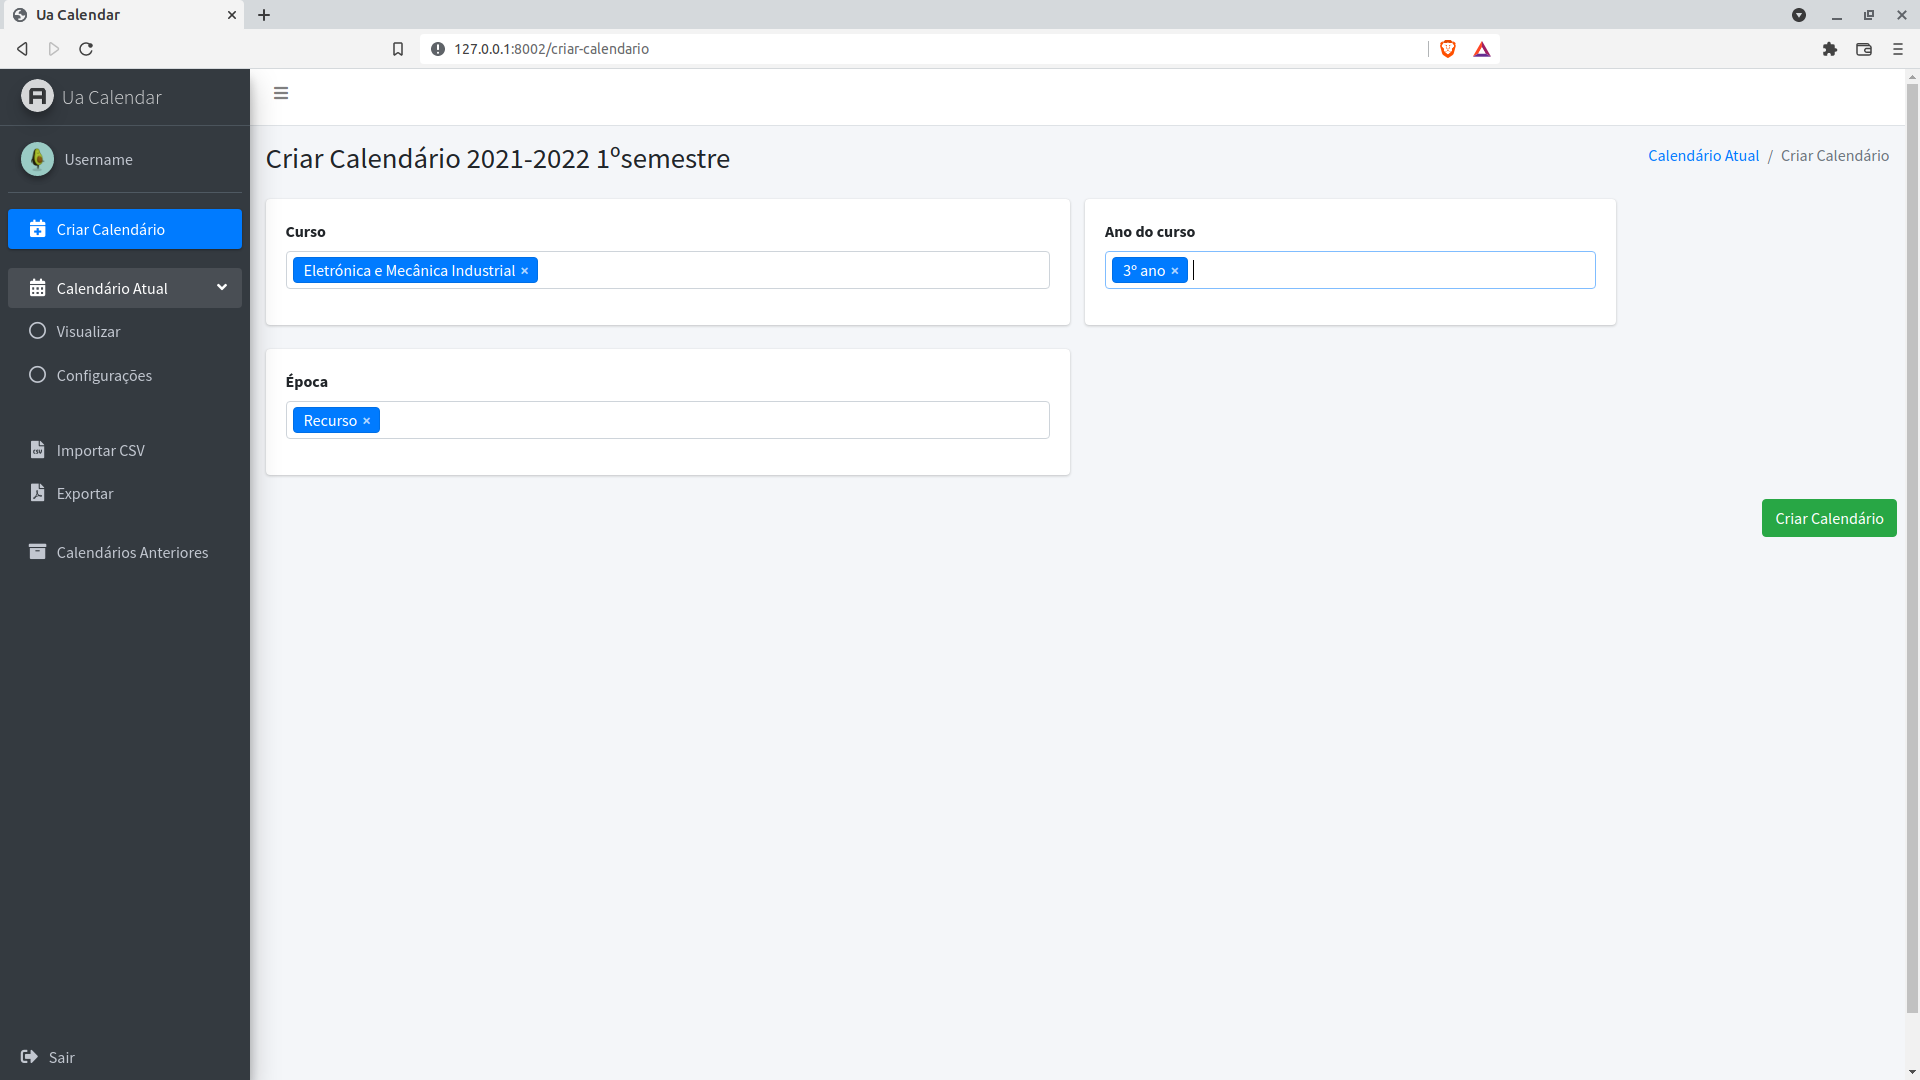
\includegraphics[width=0.8\textwidth,height=0.8\textheight,keepaspectratio]{image/PrototipoAFNF/criarCalendario}
	 	\caption{Página para criar os calendários}
	 	\label{criarCalendario}
	 \end{figure}
 
 	Depois de marcar os exames - como se pode visualizar na figura \ref{marcarExames} - o utilizador pode exportar para .pdf cada um ou vários calendários ao mesmo. Enquanto que nos wireframes só inseria a data de início e a data de fim da época e exportava todos os calendários que tinham as suas épocas dentro deste intervalo. Como se pode ver na figura \ref{exportarPDF}, e em outras páginas do protótipo, o utilizador pode filtrar os calendários por curso, ano letivo (uma vez que pode exportar os calendários anteriores), épocas, ano do curso e semestre. 
 	
 	 \begin{figure}[H] 
 		\centering 							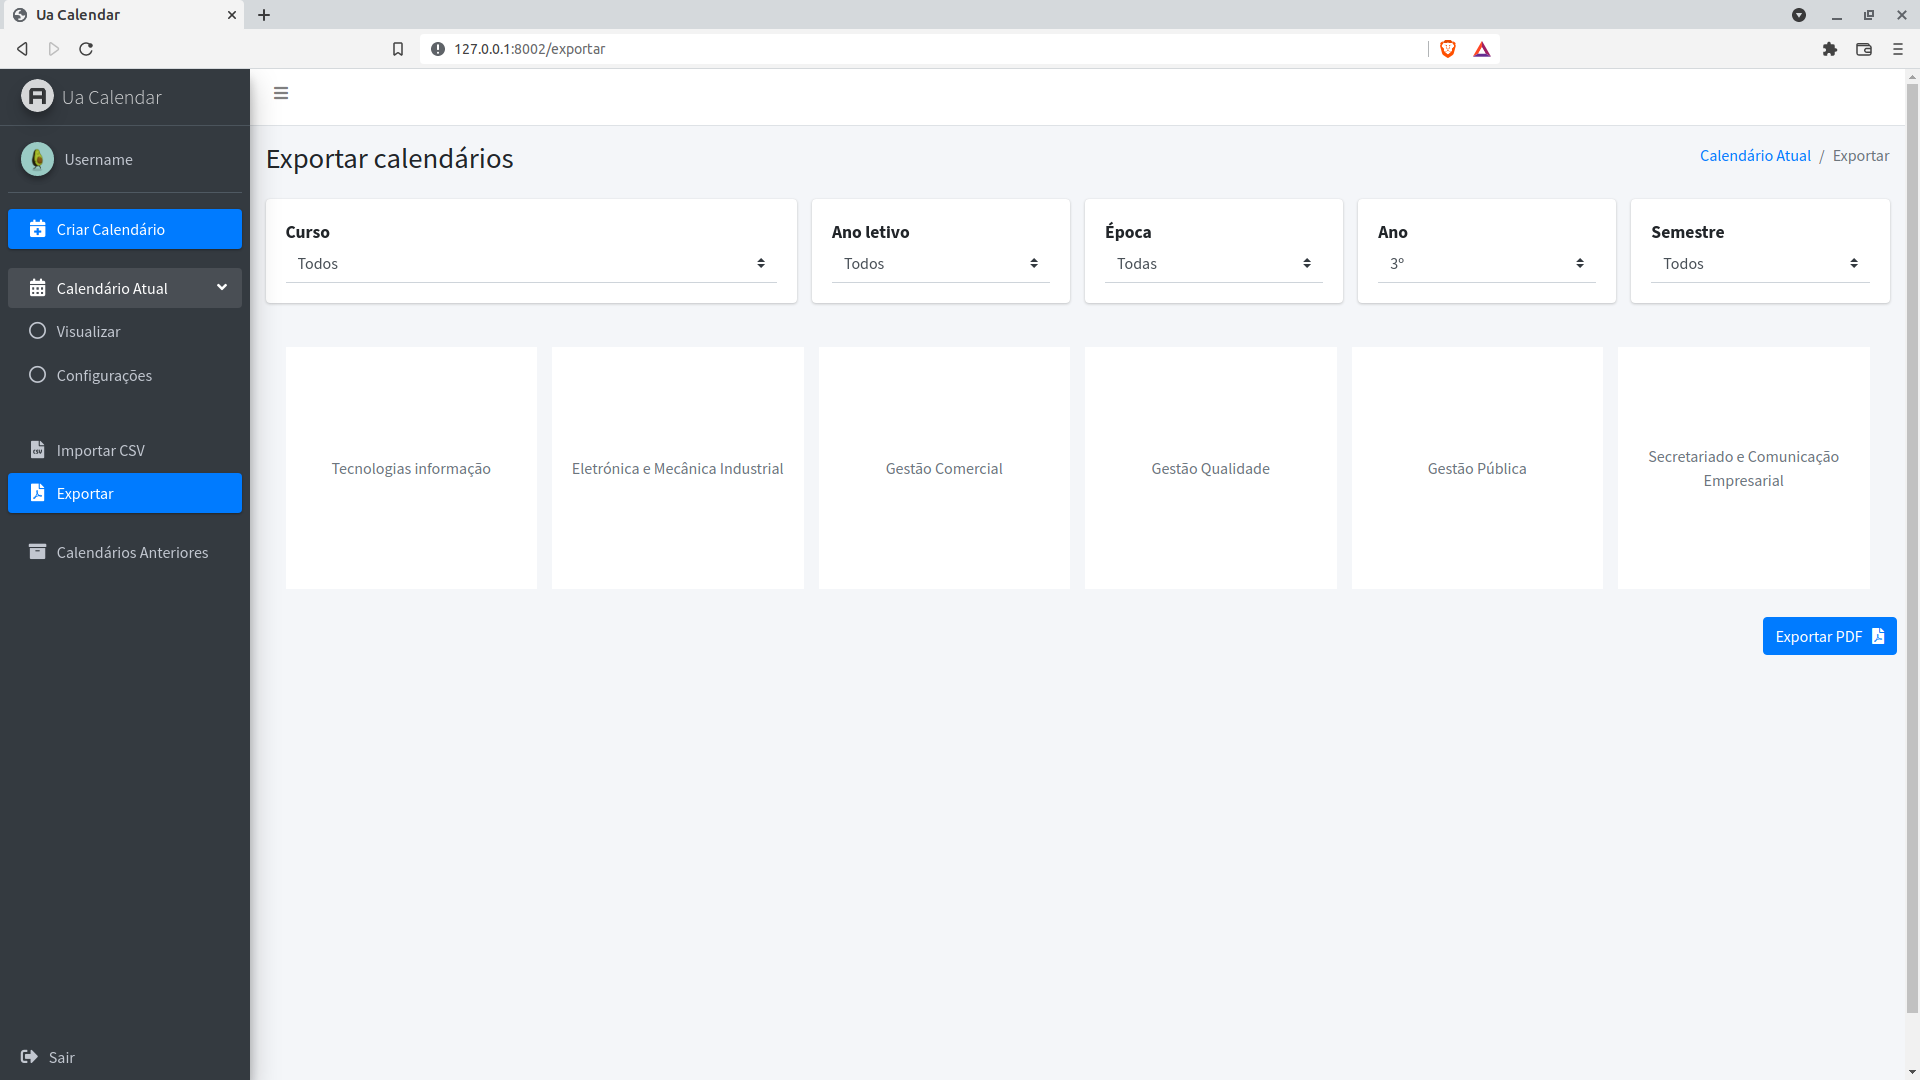
\includegraphics[width=0.8\textwidth,height=0.8\textheight,keepaspectratio]{image/PrototipoAFNF/ExportarPdf}
 		\caption{Página para exportar os calendários para .pdf }
 		\label{exportarPDF}
 	\end{figure}
 	
 	
 	Por fim o utilizador pode visualizar calendários (ver figura \ref{calendarioAnterior}) que já tenha criado anteriormente, no entanto não pode remarcar os exames, visualizar quais foram as salas e os vigilantes associados. Só mostra quando o exame foi marcado, qual a disciplina associada e em que horário. 
	
	\begin{figure}[H] 
		\centering 							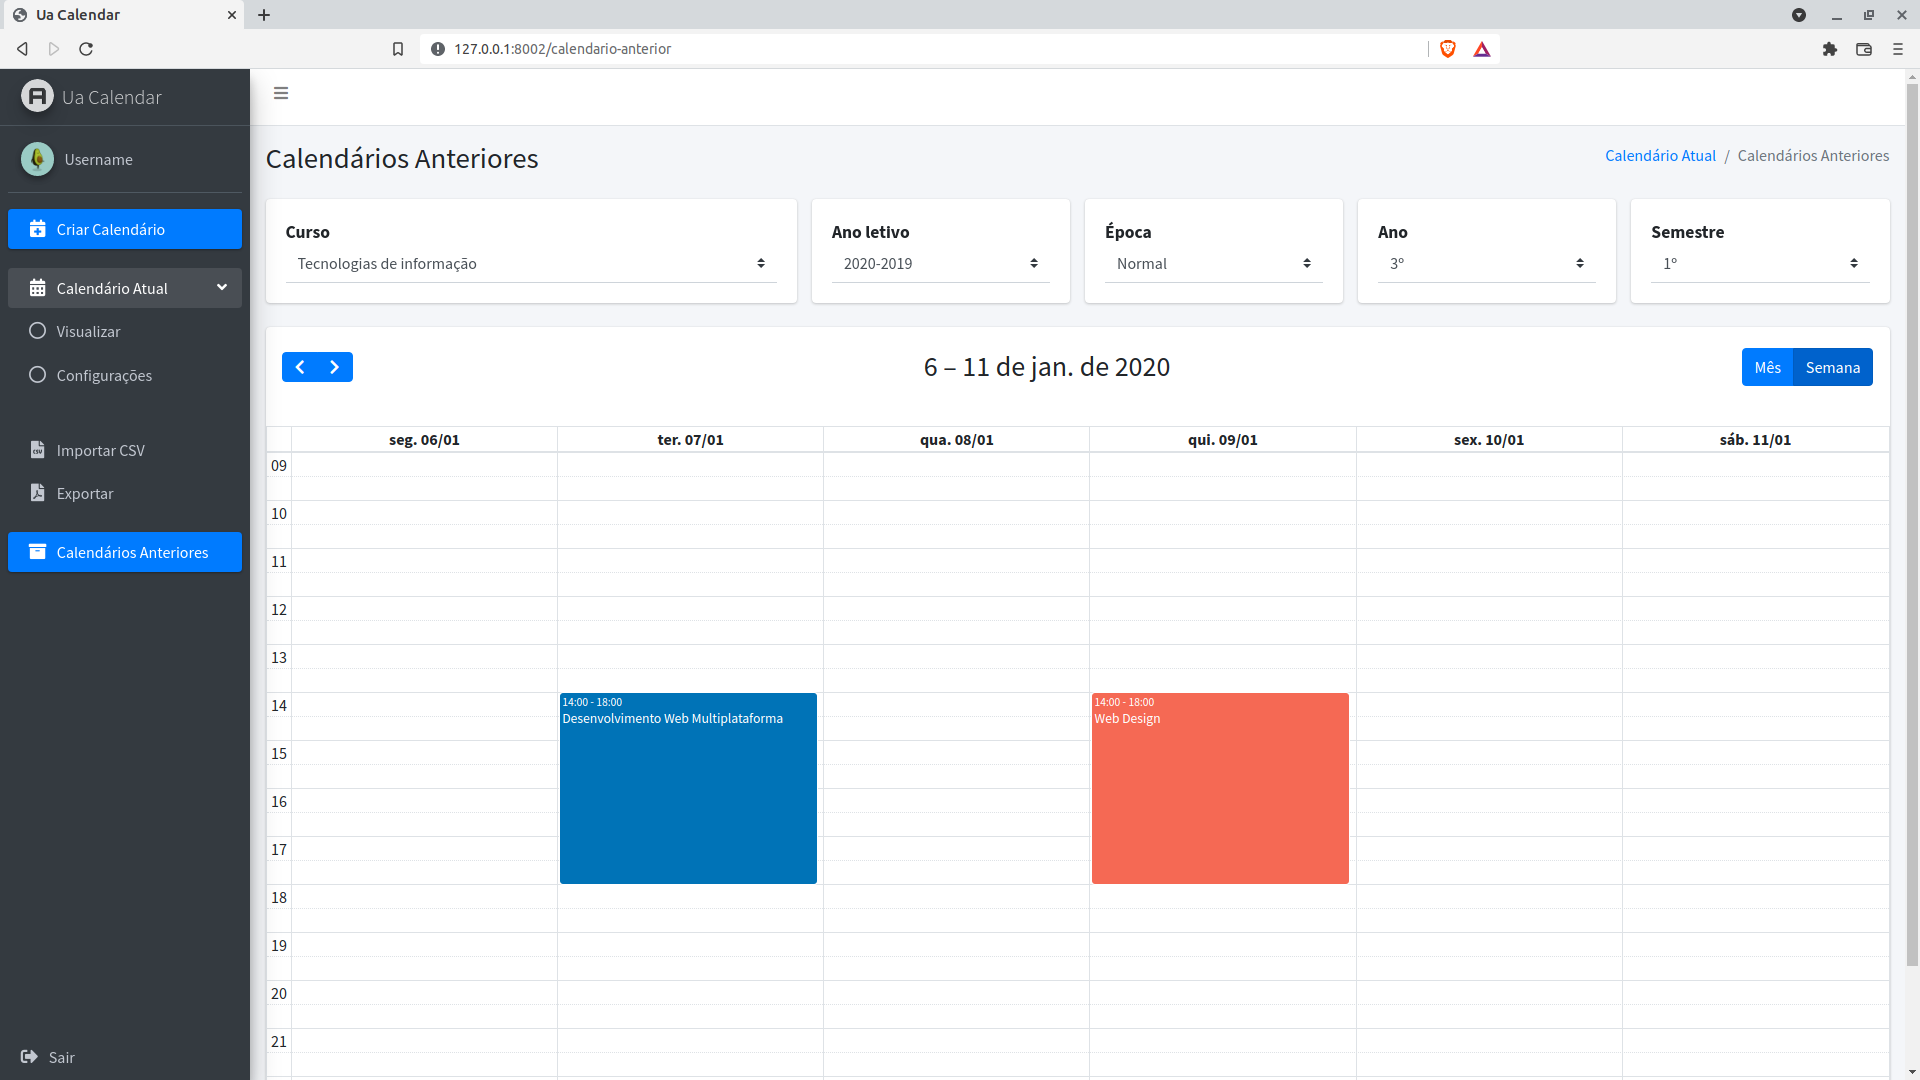
\includegraphics[width=0.8\textwidth,height=0.8\textheight,keepaspectratio]{image/PrototipoAFNF/calendarioAnterior}
		\caption{Página para visualizar o calendário anterior }
		\label{calendarioAnterior}
	\end{figure}

>>>>>>> Stashed changes
	\subsection{Guia de estilos}
	\subsection{Testes}
	
	Tal como no teste anterior - no primeiro protótipo - foi realizado uma sessão de avaliação para avaliar todas as alterações ocorridas depois do último teste e também durante o desenvolvimento do protótipo de alta fidelidade. Sendo assim a sua preparação foi idêntica e o número de participantes também (tendo o guião de participante e o guião do moderador que se mantém igual aos guiões do Anexo A e B, exceto as tarefas), alterando somente as tarefas atribuídas a cada um dos participantes: 
	
	\begin{itemize}
		\item Efetuar Login;
		\item Importar ficheiro .csv;
		\item Criar um novo calendário para o curso de Ti;
		\item Marcar exame de Web Design no dia 4 de janeiro de 2021 às 9h da manhã;
		\item Alterar professor de Economia I para Ricardo Marau;
		\item Exportar para .pdf o calendário de Tecnologias de Informação;
		\item Visualizar o calendário de 2019/2020 de Tecnologias de Informação;
		\item Sair da sessão.
		
	\end{itemize}
	
	Ao longo da sessão foram criadas duas grelhas de observação - resultante da junção de todas as grelhas de observação que se encontram no Anexo F.
	
	
	\subsubsection{Análise de resultados}
	
	Após o término da sessão foi criada uma lista com todas as alterações que têm de ser feitas antes da segunda sessão de avaliação. Essa lista se transformou na tabela \ref{analisederesultados} em que está divida em várias categorias: configurações, calendário atual,menu, importar csv, criar calendário, exportar para pdf e outros.
	

	\begin{center}
		\label{analisederesultados}
		\begin{longtable}{|m{2.2cm}|m{12cm}|}
			\caption{Análise de resultados da segunda sessão de avaliação}\\
			
			\hline			
			 \textbf{Categoria}&\textbf{Descrição da alteração} \\
			\hline
			
			\multirow{4}{2cm}{Configurações}& Trocar a cor dos icons consoante se está a editar ou não (e colocar um icon para editar as informações) \\
			
			& Configurar as disciplinas que são opção \\
			
			&Tornar mais visível que as configurações são editáveis \\
			
			&Tornar as tabs mais visíveis\\
			
			\hline
			\multirow{8}{2cm}{Calendário atual}& Retirar a vista mensal \\
			& Mostrar no exame marcado o número de salas atribuídas ao exame\\
			& Colocar só 3 períodos: manhã, tarde e noite\\
			& Mostrar apenas as disciplinas ativas naquela época\\
			& Vista do calendário para duas semanas\\
			&Alterar o dia do exame através de um aopção no popup\\
			&Mostrar a cinzento os dias que não pertencem à época escolhida\\
			&Aparecer um aviso de que falta marcar docentes e salas após ter marcado um exame\\
			
			\hline
			
			\multirow{2}{2cm}{Menu} &Mudar o nome de ``visualizar" para marcação de exames\\
			&Mudar o nome de ``configurações" para dados auxiliares\\
			\hline
			Importar CSV & ter uma preview dos dados importados.\\
			\hline
			\multirow{2}{2cm}{Criar calendário} & Colocar uma checkbox na múltipla seleção para tornar mais perceptível da sua funcionalidade.\\
			& Verificar se tem o csv e senão pedir para importar\\
			\hline
			Exportar para pdf & Mostrar em forma de lista com uma checkbox todos os cursos que se quer exportar\\
			\hline
			Outros & Criar um sumário de incompatibilidades\\
			\hline
		\end{longtable}
	\end{center}
	
	
	
	 
	
	\chapter{Implementação do modelo de dados persistentes}
	\section{Estrutura da base de dados}
	\subsection{Base de dados - factories}
	\section{Arquitetura do sistema - Modelo MVC}
	\subsection{Models e Controllers}
	
	\chapter{Primeira versão da aplicação}
	\section{Implementação de funcionalidades}
	
	\chapter{Testes finais}
	\section{Testes com potenciais clientes}
	\section{Testes de acessibilidade}
	\section{Análise de resultados}
	
	\chapter{Lançamento da versão final}
	\section{Alocação da aplicação no servidor}
	
	
	\chapter{Reflexão crítica e conclusão}
	
	

	\bibliographystyle{ieeetr}
	\bibliography{citations}
	\pagenumbering{roman}
	\pagestyle{empty}
	
	\chapter*{Anexo A}
		\section*{Guião da sessão de avaliação do protótipo de baixa fidelidade não funcional}
		\subsection*{Documento de apoio ao moderador}
			
		
		\subsubsection*{Introdução}
	O presente guião tem como função principal auxiliar/guiar o moderador para a sessão de avaliação da aplicação “UACalendar”. O conjunto de tarefas que se seguem irão servir para avaliar a eficácia, eficiência e satisfação do utilizador perante a interface idealizada, tendo como objetivo a aplicação de melhorias conforme o feedback dos participantes.
	Todos os dados recolhidos na realização desta sessão de avaliação serão tratados de forma anónima e utilizados apenas no âmbito deste projeto.
		
		
	\subsubsection*{Preparação da sessão de avaliação}
			Para que a realização desta sessão de avaliação seja possível, será necessário que cada um dos participantes tenha acesso a:
	
	\begin{itemize}
		\item Um computador com um browser instalado;
		\item Um periférico de entrada, tal como por exemplo um rato, touchpad, etc.;
		\item Ligação à internet para acesso aos \href{https://www.figma.com/file/nhb5nnIrt3fdDoQhYpsN80/Calendario?node-id=9\%3A154}{\textbf{wireframes}}.
	\end{itemize}

\subsubsection*{Durante a sessão de avaliação}	
Durante a sessão de avaliação o moderador deverá:

	\begin{itemize}
		\item Receber o participante de forma cordial e realizar as devidas apresentações das pessoas envolvidas na sessão (moderador, observadores e participante);
		\item Tentar deixar os participantes o mais à vontade possível e relembrar que não existem respostas certas ou erradas;
		\item Explicar o que vai ser testado e quais os objetivos desta sessão;
		\item Encorajar o participante a pensar em voz alta, permitindo que tanto o moderador como os observadores possam acompanhar o raciocínio do mesmo;
		\item Guiar os participantes durante a sessão de avaliação, porém em momento algum deverá ajudar/influenciar os participantes na conclusão das tarefas apresentadas, caso o faça, incorrerá na adulteração dos resultados pretendidos;
		\item Encerrar a sessão de avaliação.
	\end{itemize}
	
	\subsubsection*{Tarefas a serem pedidas ao utilizador participante}	
	O utilizador participante deverá:
	
		\begin{itemize}
			\item Verificar o calendário final de Ti do ano letivo 2019/2020;
			\item Importar ficheiro .csv;
			\item Verificar individualmente quantas disciplinas, salas e docentes existem;
			\item Pesquisar por "Ti" na barra de pesquisa e abrir o calendário "Ti - 1º Ano - 1º Semestre";
			\item Criar um novo calendário para o curso de Ti;
			\item Mova matemática para o período da manhã do dia 14;
			\item Colocar "Segurança Inf." num período da noite;
			\item Exportar para um .pdf;
			\item Fazer log out.
		\end{itemize}
	
	
	\chapter*{Anexo B}
		\section*{Guião da sessão de avaliação do protótipo de baixa fidelidade não funcional}
		\subsection*{Documento de apoio ao utilizador participante}
			
		
		\subsubsection*{Introdução}
			O presente guião tem como função principal guiar o utilizador participante durante a sessão de avaliação da aplicação “UACalendar”. O conjunto de tarefas que se seguem irão servir para obter a opinião do utilizador participante perante a interface idealizada, tendo como objetivo a aplicação de melhorias conforme o feedback do mesmo. Todos os dados recolhidos na realização desta sessão de avaliação serão tratados de forma anónima e utilizados apenas no âmbito deste projeto.
	
		\subsubsection*{Tarefas a realizar}	
	\begin{itemize}
		\item Verifique o calendário final de Ti do ano letivo 2019/2020;
		\item Importe ficheiro .csv;
		\item Verifique individualmente quantas disciplinas, salas e docentes existem;
		\item Pesquise por "Ti" na barra de pesquisa e abrir o calendário "Ti - 1º Ano - 1º Semestre";
		\item Crie um novo calendário para o curso de Ti;
		\item Mova matemática para o período da manhã do dia 14;
		\item Coloque "Segurança Inf." num período da noite;
		\item Exporte para um .pdf;
		\item Faça log out.
	\end{itemize}

	
	\chapter*{Anexo C}
	\section*{Grelhas de observação da avaliação do protótipo de baixa fidelidade não funcional}
		\begin{landscape}
		\clearpage
			\pagestyle{empty}
			\begin{figure}[H] 
				\centering 							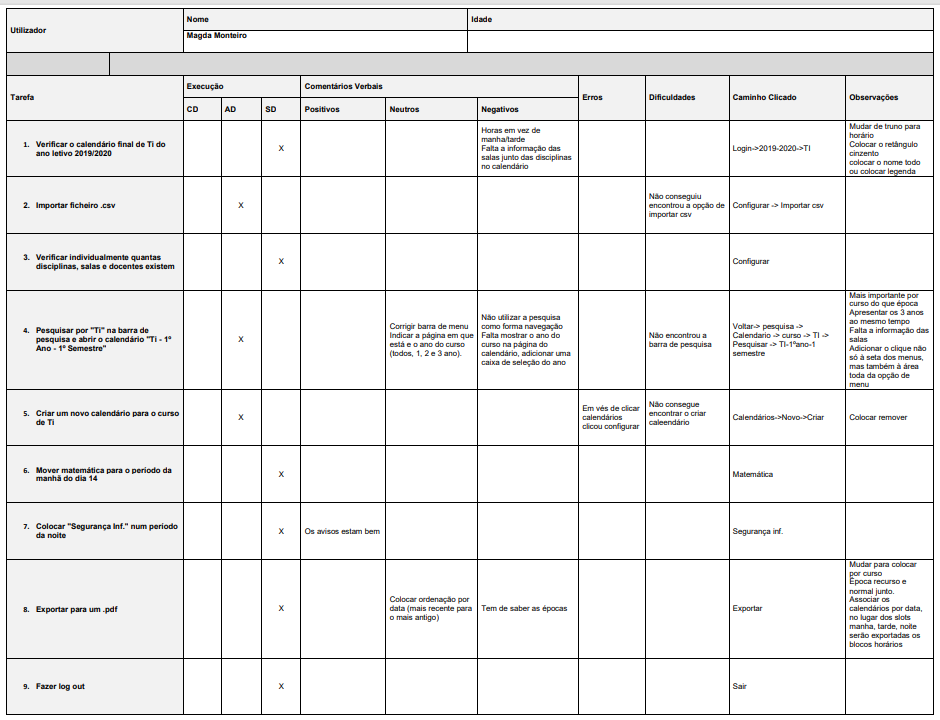
\includegraphics[width=1.23\textwidth,height=1.23\textheight,keepaspectratio]{image/testes_prototipo_baixo_fidelidade/grelha_observadores_magda}
				\caption{Grelha de observação do participante 1}
				
			\end{figure}
			\begin{figure}[H] 
				\centering 							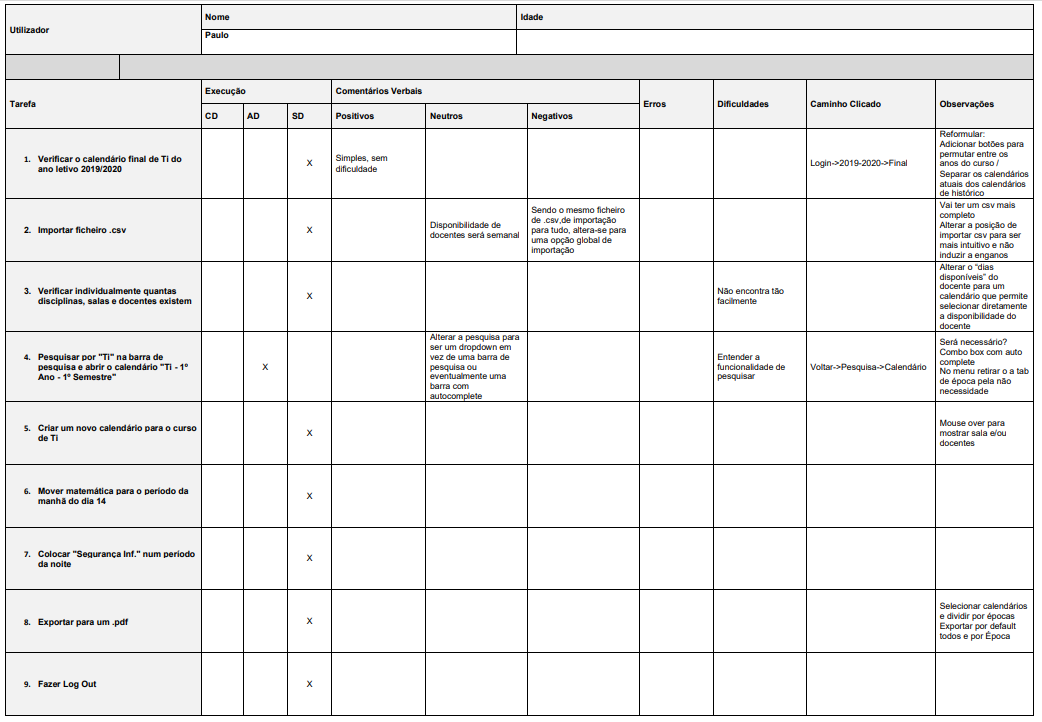
\includegraphics[width=1.4\textwidth,height=1.4\textheight,keepaspectratio]{image/testes_prototipo_baixo_fidelidade/grelha_observadores_paulo}
				\caption{Grelha de observação do participante 2}
				
			\end{figure}
		\end{landscape}

	\chapter*{Anexo F}
		\section*{Grelhas de observação da avaliação do protótipo de alta fidelidade não funcional}
		\begin{landscape}
			\clearpage
			\pagestyle{empty}
			
			\begin{figure}[H] 
				\centering 							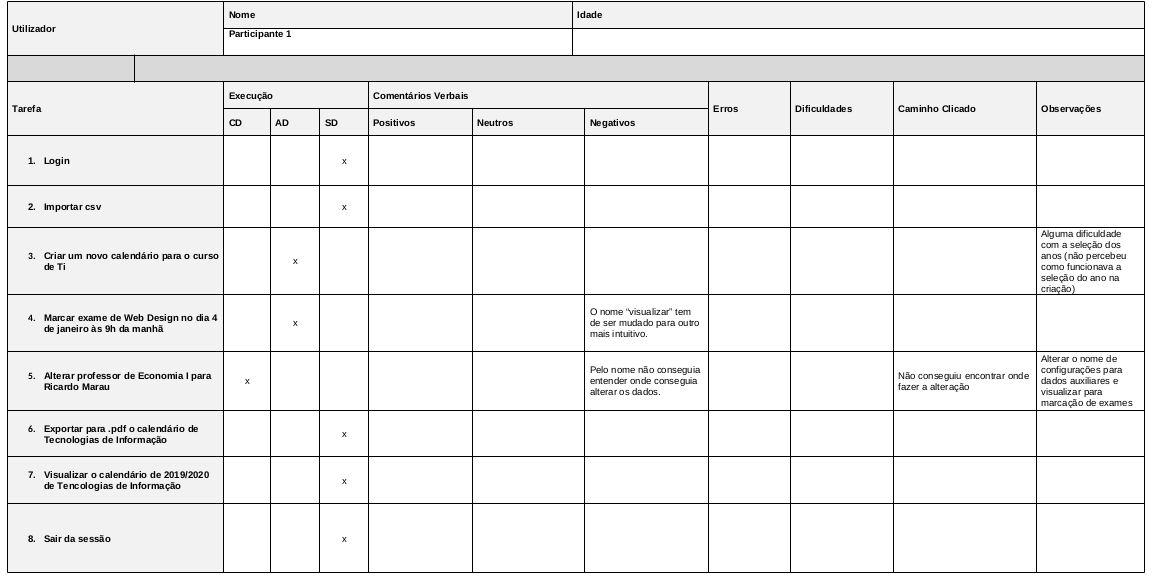
\includegraphics[width=1.4\textwidth,height=1.4\textheight,keepaspectratio]{image/Testes segunda_sessão/GrelhaObservadorParticipante1}
				\caption{Grelha de observação do participante 1}
				
			\end{figure}
			\begin{figure}[H] 
				\centering 							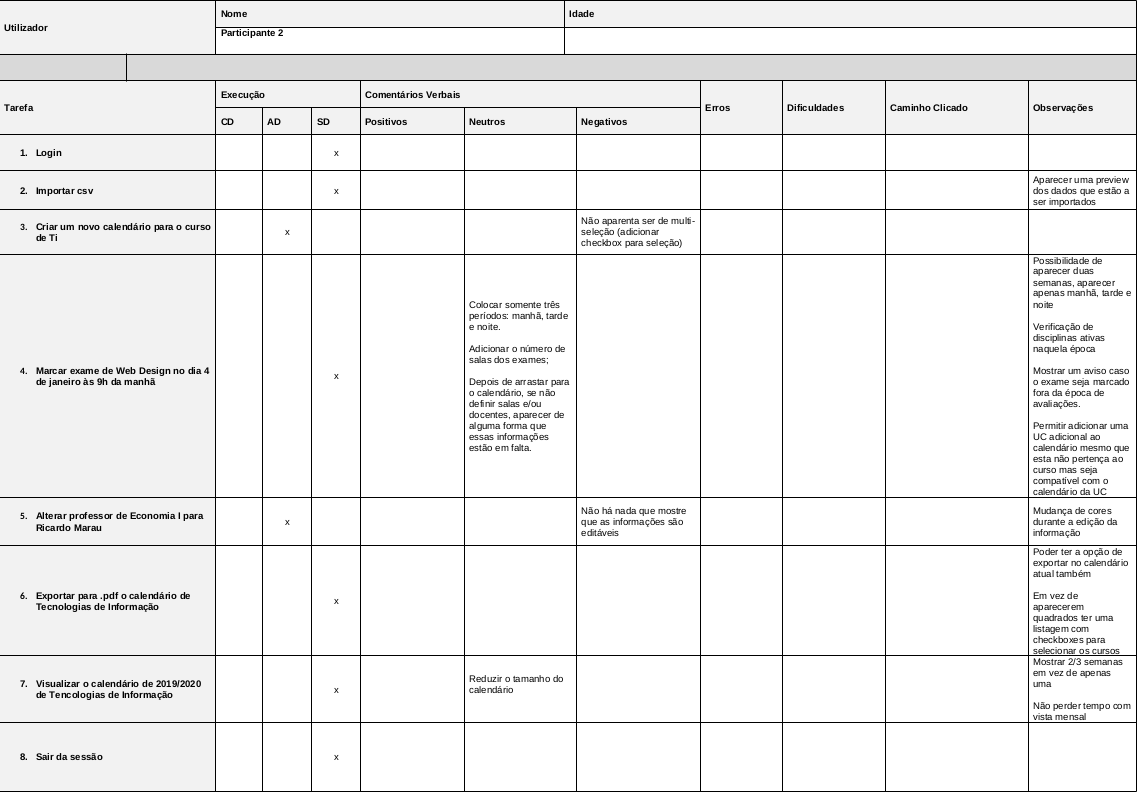
\includegraphics[width=1.4\textwidth,height=1.4\textheight,keepaspectratio]{image/Testes segunda_sessão/GrelhaObservador_Participante2}
				\caption{Grelha de observação do participante 2}
			\end{figure}
			
			
			\end{landscape}
	
\end{document}	
	
	
	
	
